\documentclass[11pt,a4paper]{article}

\usepackage{xltxtra} 
\usepackage{xgreek} 
\usepackage{graphicx}
\usepackage{float}
\usepackage{indentfirst}
\usepackage[a4paper, total={6in, 8in}]{geometry}
\usepackage[dvipsnames]{xcolor}
\usepackage{enumitem}
\usepackage[bottom]{footmisc}
\usepackage{amsmath}
\usepackage{array}
\setitemize{noitemsep,topsep=0pt,parsep=0pt,partopsep=0pt}
\usepackage{geometry}
 \geometry{
 a4paper,
 total={170mm,257mm},
 left=20mm,
 top=20mm,
 }

\setmainfont[Mapping=tex-text]{GFS Didot} 


\renewcommand{\figurename}{Σχήμα}

\title{Προηγμένες Τεχνικές Επεξεργασίας Σήματος\\Δεύτερη Εργασία}

\author{Γραικός Αλέξανδρος 8128, \\Θώμος Μάριος 8384}

\date{\today}

\begin{document}
\maketitle

\section*{Σήματα που επιλέχθηκαν}
Τα σήματα που επιλέξαμε να αναλύσουμε είναι τα \textbf{112}, \textbf{123}, \textbf{118}, \textbf{217}, \textbf{221}. Τα σήματα 1xx λήφθηκαν τυχαία από ασθενείς με διάφορες παθήσεις ενώ τα 2xx έχουν επιλεχθεί έτσι ώστε να περιέχουν σπάνια καρδιακά φαινόμενα με ιδιαίτερο ενδιαφέρον στη μελέτη τους.

\begin{center}
\begin{tabular}{| >{\centering\arraybackslash}m{1cm} | >{\centering\arraybackslash}m{15cm}|} 
 \hline
 Σήμα & Χαρακτηριστικά \\ 
 \hline 
 112 &  Το σήμα του ασθενούς 112 είναι φυσιολογικό, με μερικές μόνο δυσμορφίες λόγω πρόωρων κολπικών συστολών (APCs). Ο καρδιακός ρυθμός είναι σταθερός και εμφανίζεται θόρυβος σε δύο μικρές περιοχές. Αναλύοντας το σήμα αυτό, θα δοκιμάσουμε τις μεθόδους ανάλυσης πάνω σε μια απλή περίπτωση ασθενούς. Από τον ασθενή 112 θα αναλύσουμε τα σήματα και από τα δύο άκρα για να εντοπίσουμε τυχόν διαφορές που μπορεί να εμφανίζονται μεταξύ τους. \\
 \hline
 123 & Ο ασθενής 123 εμφανίζει κυρίως κανονικούς παλμούς με μερικές πρόωρες κοιλιακές συστολές (PVCs). Έχει σταθερό και χαμηλό καρδιακό ρυθμό με εξαίρεση κάποια σημεία όπου εμφανίζεται φλεβοκομβική αρρυθμία. Από την ανάλυση του σήματος αυτού, θα μπορούμε να εξετάσουμε τις διαφορές που θα προκύψουν λόγω της αρρυθμίας σε σύγκριση με φυσιολογικούς ασθενείς. \\
 \hline
 118 & Κατά την καταγραφή του σήματος του ασθενούς 118, εμφανίζεται αποκλεισμός δεξιού σκέλους καρδιάς (RBBB), καθώς και πρόωρες κοιλιακές και κολπικές συστολές. Ο ασθενής έχει σταθερό καρδιακό ρυθμό και στο σήμα επικάθεται θόρυβος σε μεμονωμένες περιοχές. Λόγω του RBBB και τον πολλαπλών δυσμορφιών του καρδιογραφήματος, η ανάλυση του σήματος αυτού θα αποδώσει μοναδικά αποτελέσματα. \\
 \hline
 217 & Οι παλμοί του ασθενούς 217 έχουν την ιδιαιτερότητα οτι αποτελούνται από έναν συνδυασμό κανονικών και οδηγούμενων από το βηματοδότη παλμών. Μαζί με την εμφάνιση πρόωρων κοιλιακών συστολών, εξασφαλίζεται πλούσιο περιεχόμενο προς ανάλυση. Ο ασθενής πάσχει από κολπική μαρμαρυγή και αρχικά ο καρδιακός του ρυθμός είναι ασταθής. Έπειτα, ο βηματοδότης σταθεροποιεί τον παλμό του, δίνοντας μας την δυνατότητα να συγκρίνουμε μέσα από τις μεθόδους ανάλυσης, τις διαφορές μεταξύ των δύο αυτών καταστάσεων. \\
 \hline
 221 & Ο ασθενής 221 εμφανίζει κανονικούς παλμούς και δυσμορφίες λόγω πρόωρης κοιλιακής συστολής. Παράλληλα, παρουσιάζει αρρυθμία καθώς πάσχει από κολπική μαρμαρυγή και δεν χρησιμοποιεί βηματοδότη για σταθεροποίηση. Σε αυτήν την περίπτωση, οι μέθοδοι ανάλυσης θα εφαρμοστούν σε ένα σήμα χωρίς κάποιους σταθερούς ρυθμούς και περιμένουμε τα αποτελέσματα να μας δείξουν τις ιδιαιτερότητες αυτού του καρδιογραφήματος.\\ 
 \hline
\end{tabular}
\end{center}


\section*{Ανάλυση Σημάτων}
\subsection*{112}

% --- STFT, WDF, CWT ---
\begin{figure}[H]
\centering
\begin{minipage}{0.48\textwidth}
	\centering
	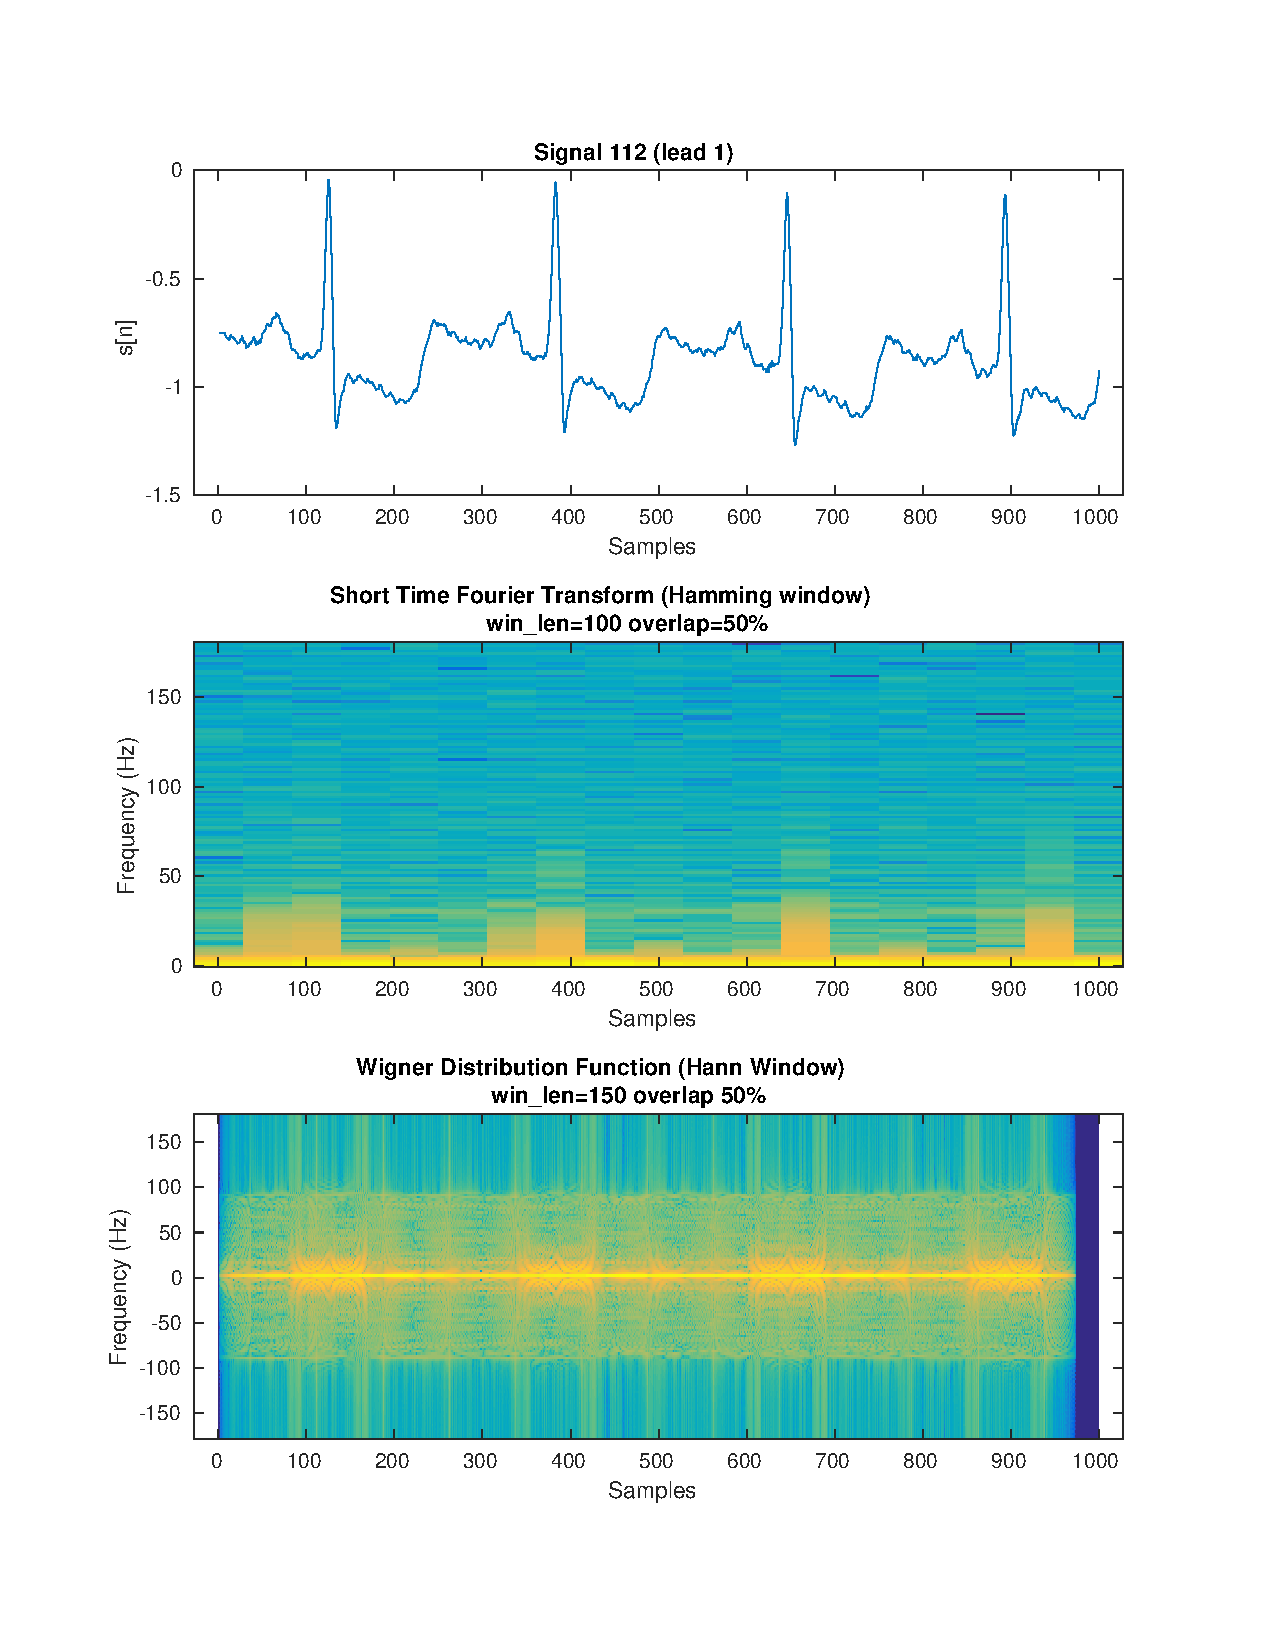
\includegraphics[width=\textwidth]{fig/112l1_stft_wdf.pdf}
	
	(α)
\end{minipage}
\begin{minipage}{0.48\textwidth}
	\centering
	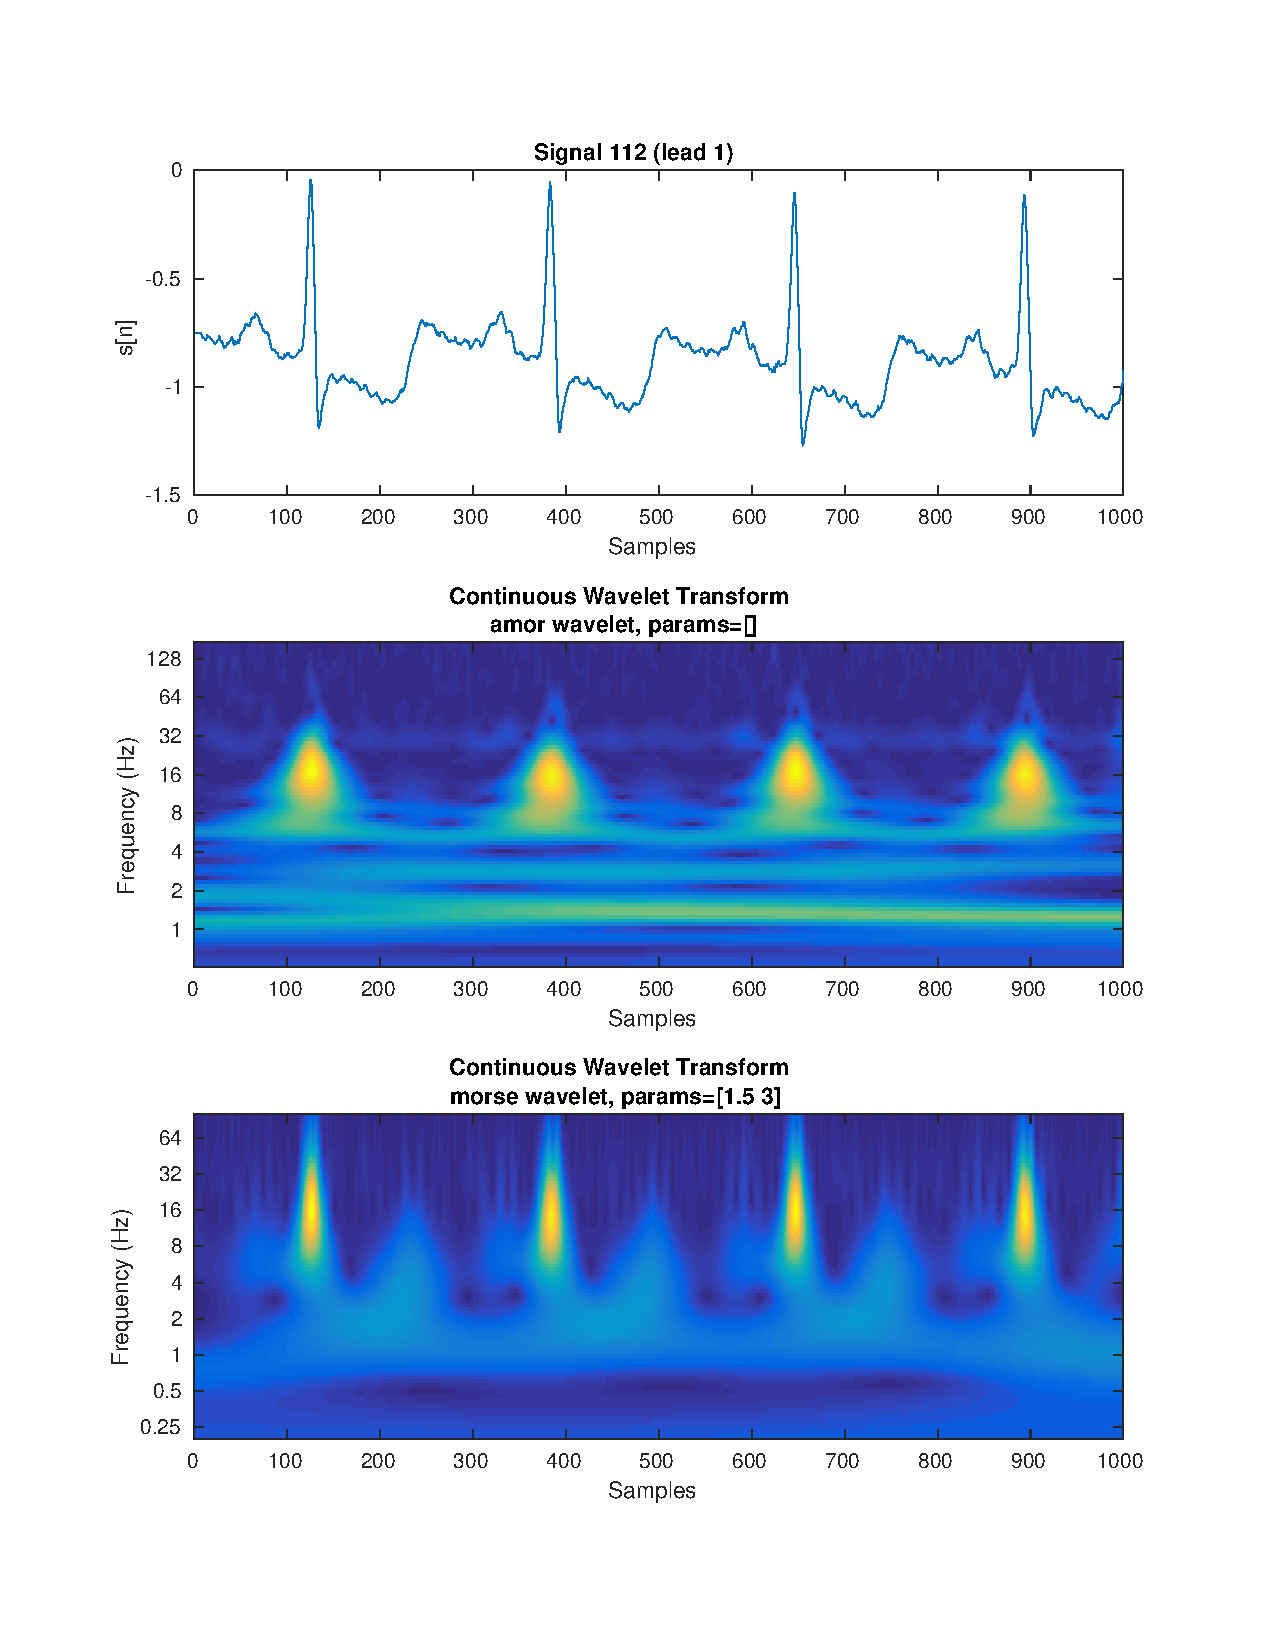
\includegraphics[width=\textwidth]{fig/112l1_cwt.pdf}
	
	(β)
\end{minipage}
\vfill
\caption{(α) Short Time Fourier Transform και Wigner Distribution Function (β) Wavelet Transform (Morlet, Morse wavelets) του σήματος.}
\label{fig:112l1_stft_wdf_wt}
\end{figure}


% --- DWT ---
\begin{figure}[H]
\centering
\begin{minipage}{0.48\textwidth}
	\centering
	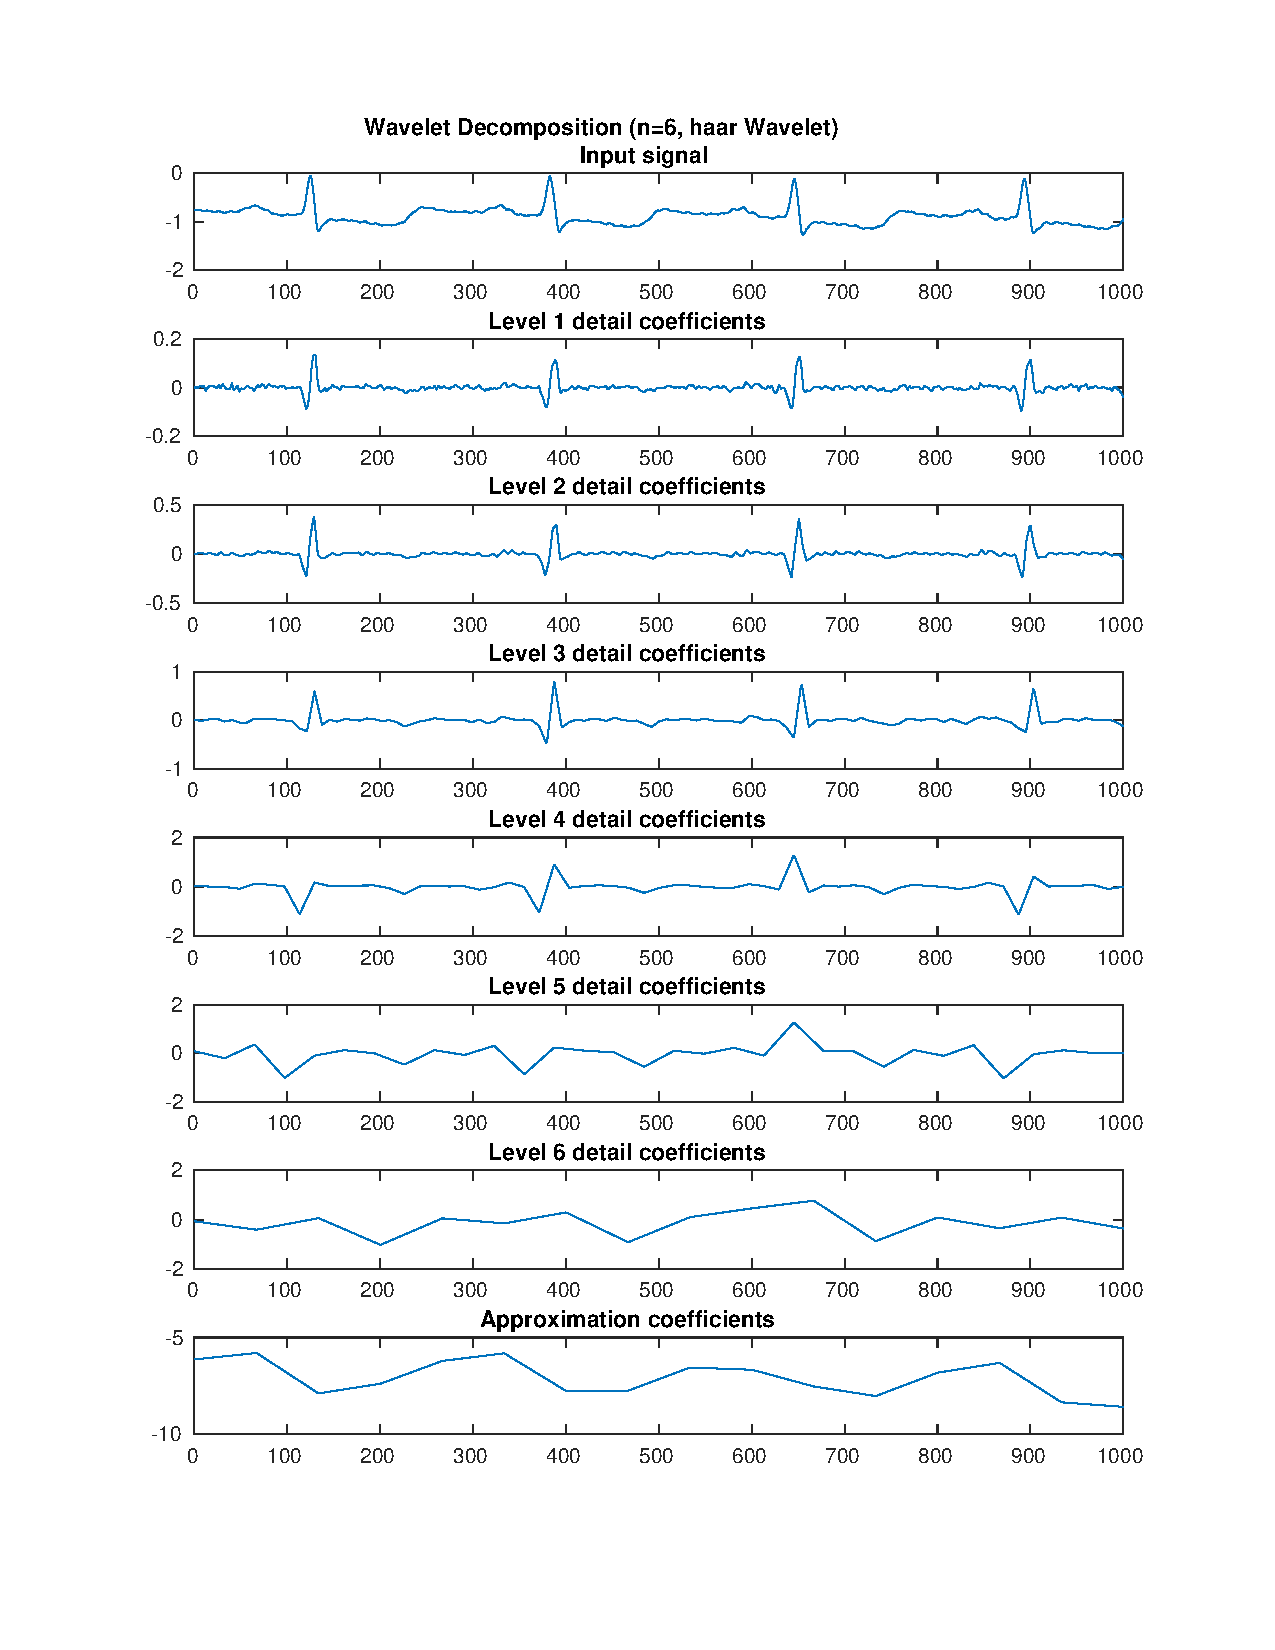
\includegraphics[width=\textwidth]{fig/112l1_dwt1.pdf}
	
	(α)
\end{minipage}
\begin{minipage}{0.48\textwidth}
	\centering
	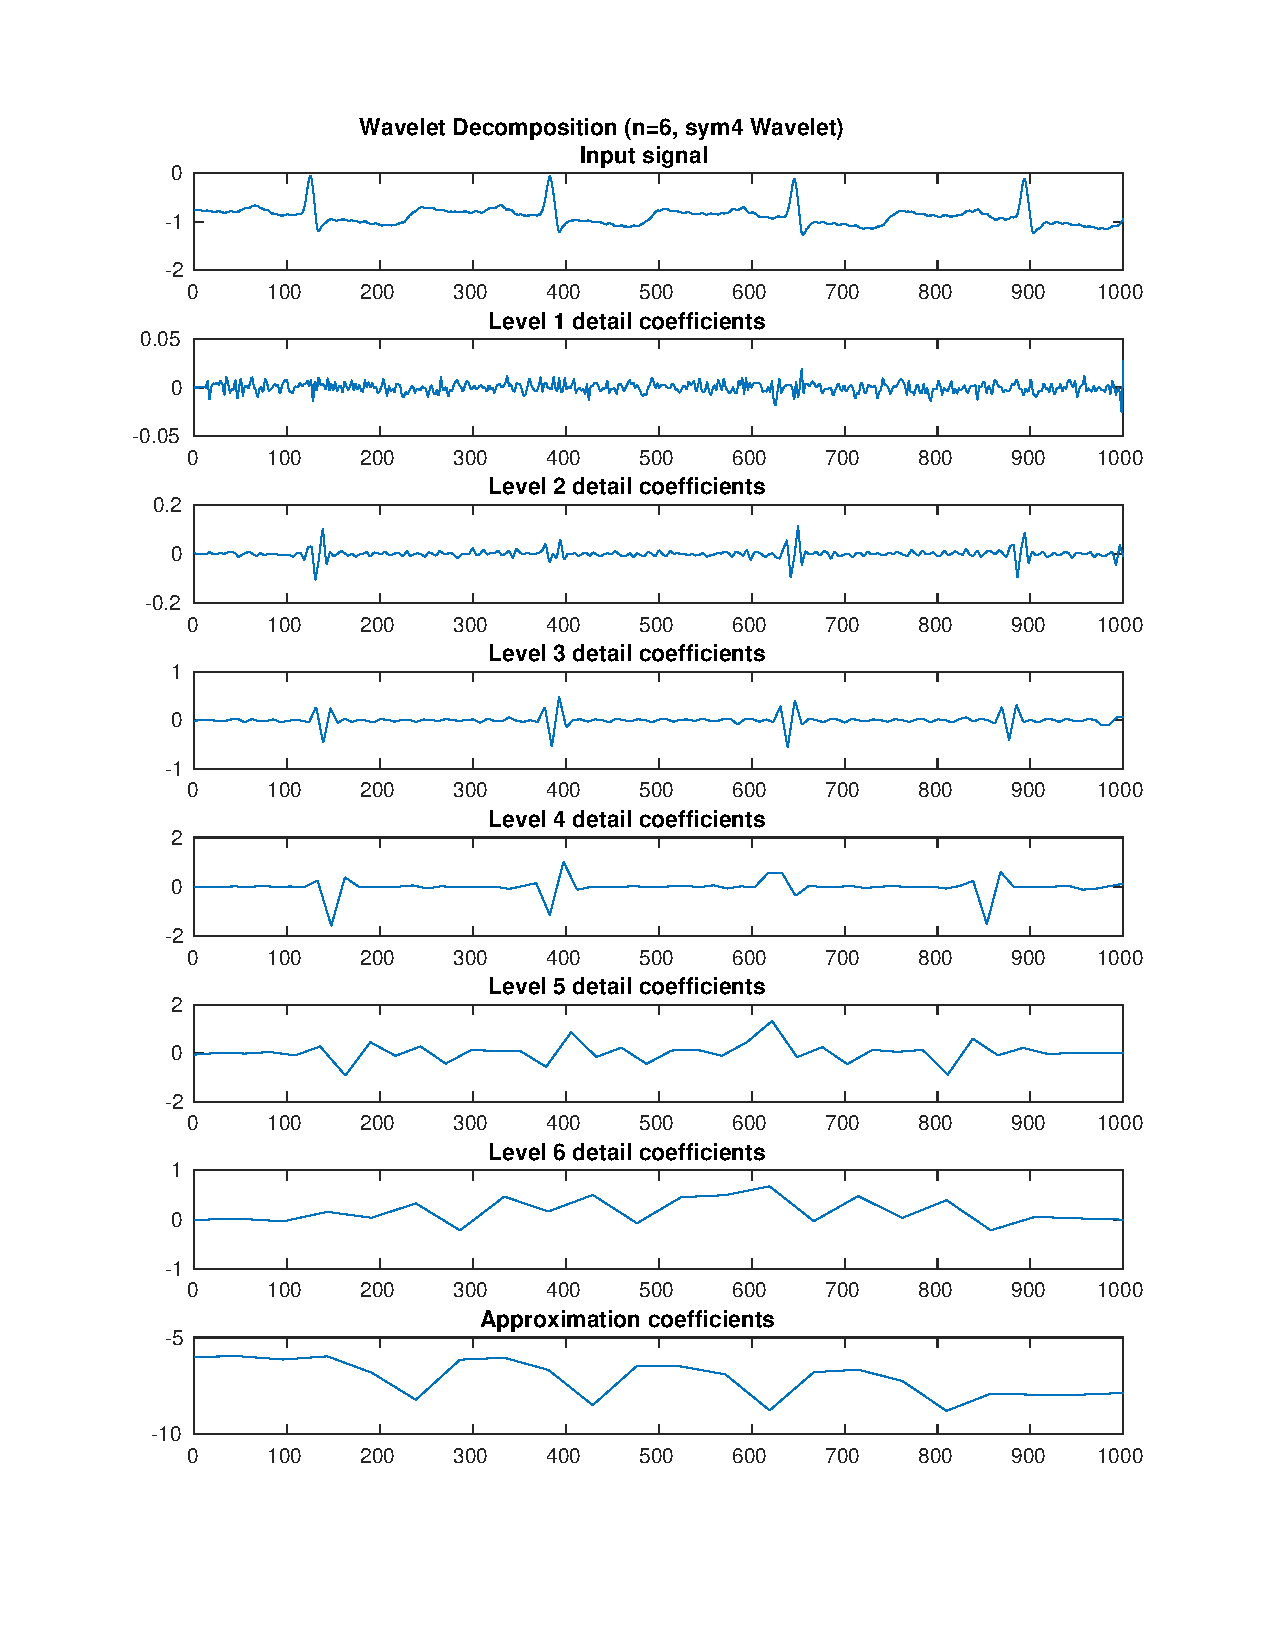
\includegraphics[width=\textwidth]{fig/112l1_dwt2.pdf}
	
	(β)
\end{minipage}
\vfill
\caption{Wavelet Decomposition του σήματος χρησιμοποιώντας wavelet (α) Haar (β) Symlet4.}
\label{fig:112l1_dwt}
\end{figure}


% --- EMD/HHT ---
\begin{figure}[H]
\centering
\begin{minipage}{0.48\textwidth}
	\centering
	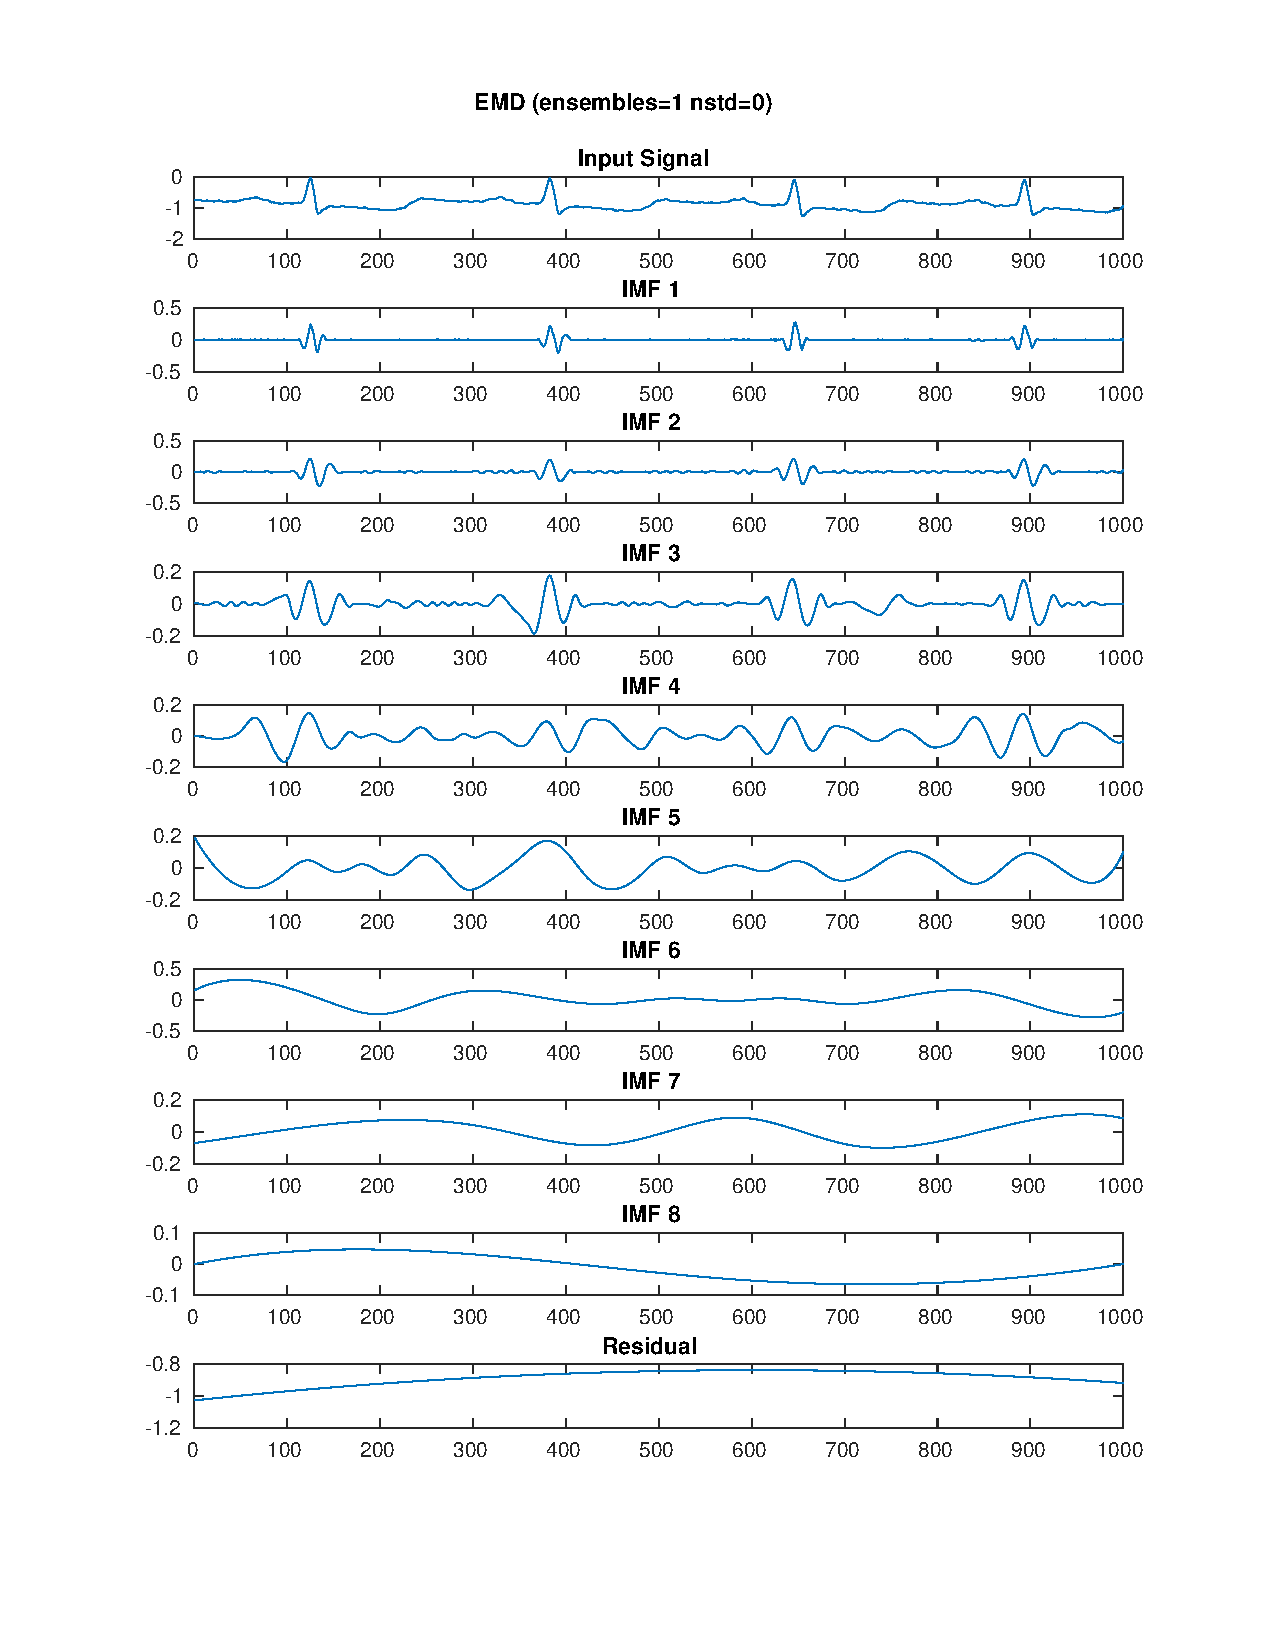
\includegraphics[width=\textwidth]{fig/112l1_emd.pdf}
	
	(α)
\end{minipage}
\begin{minipage}{0.48\textwidth}
	\centering
	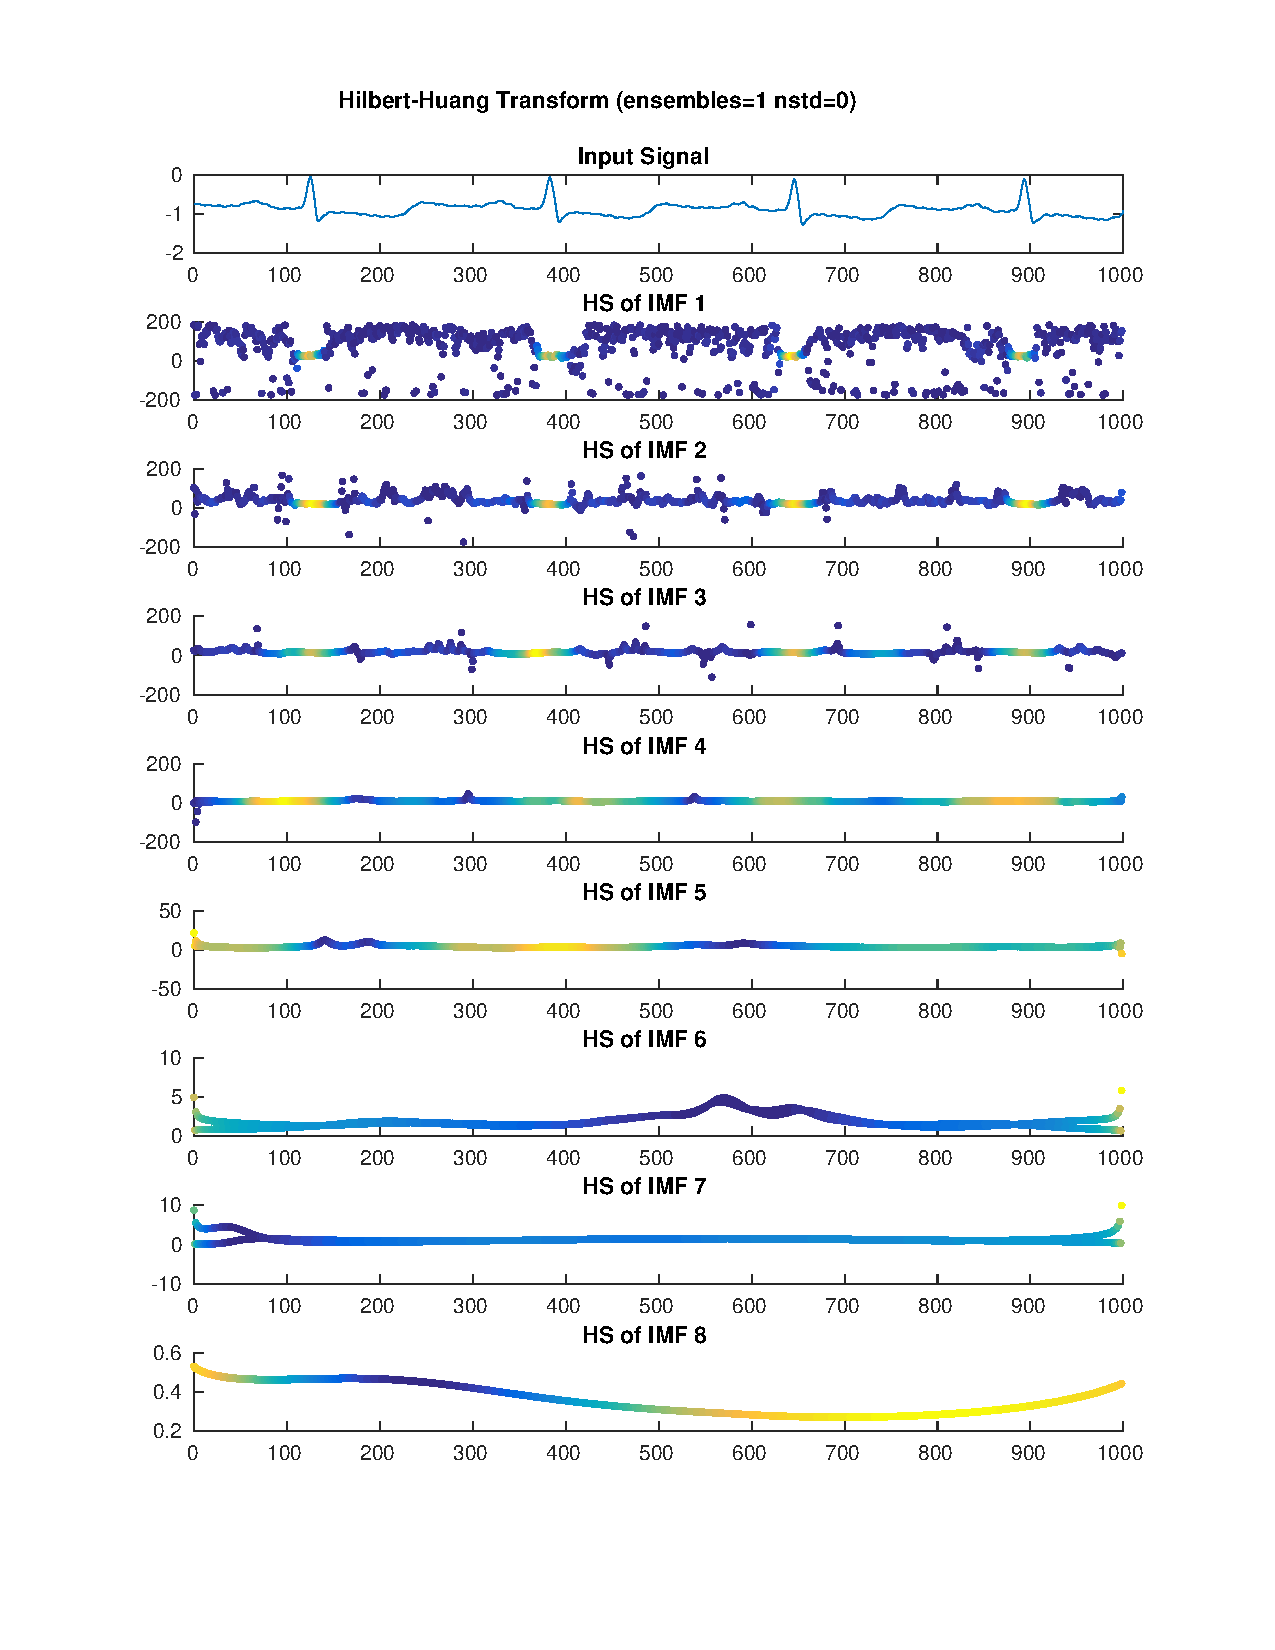
\includegraphics[width=\textwidth]{fig/112l1_hht.pdf}
	
	(β)
\end{minipage}
\vfill
\caption{(α) Emperical Mode Decomposition (β) Hilbert-Huang Transform του σήματος.}
\label{fig:112l1_hht}
\end{figure}


% --- EEMD/HHT ---
\begin{figure}[H]
\centering
\begin{minipage}{0.48\textwidth}
	\centering
	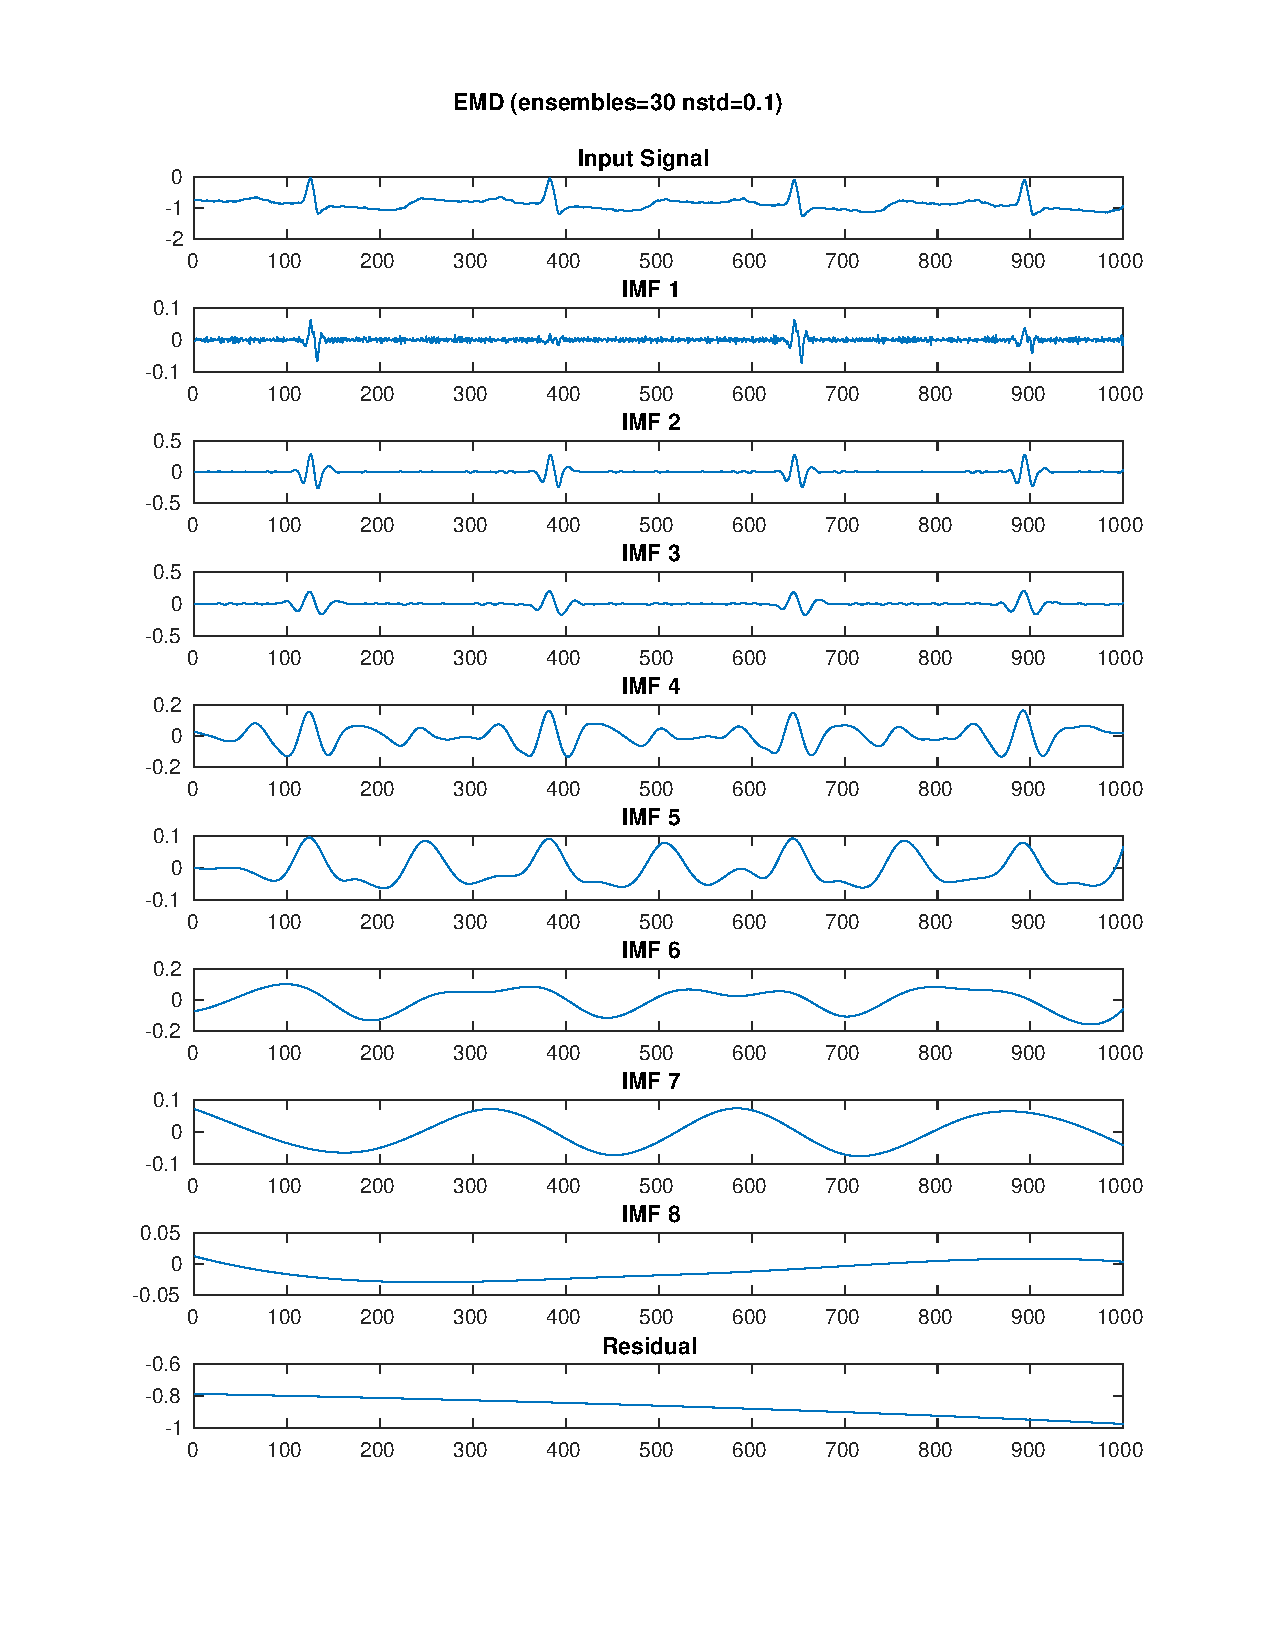
\includegraphics[width=\textwidth]{fig/112l1_emd_ensemble.pdf}
	
	(α)
\end{minipage}
\begin{minipage}{0.48\textwidth}
	\centering
	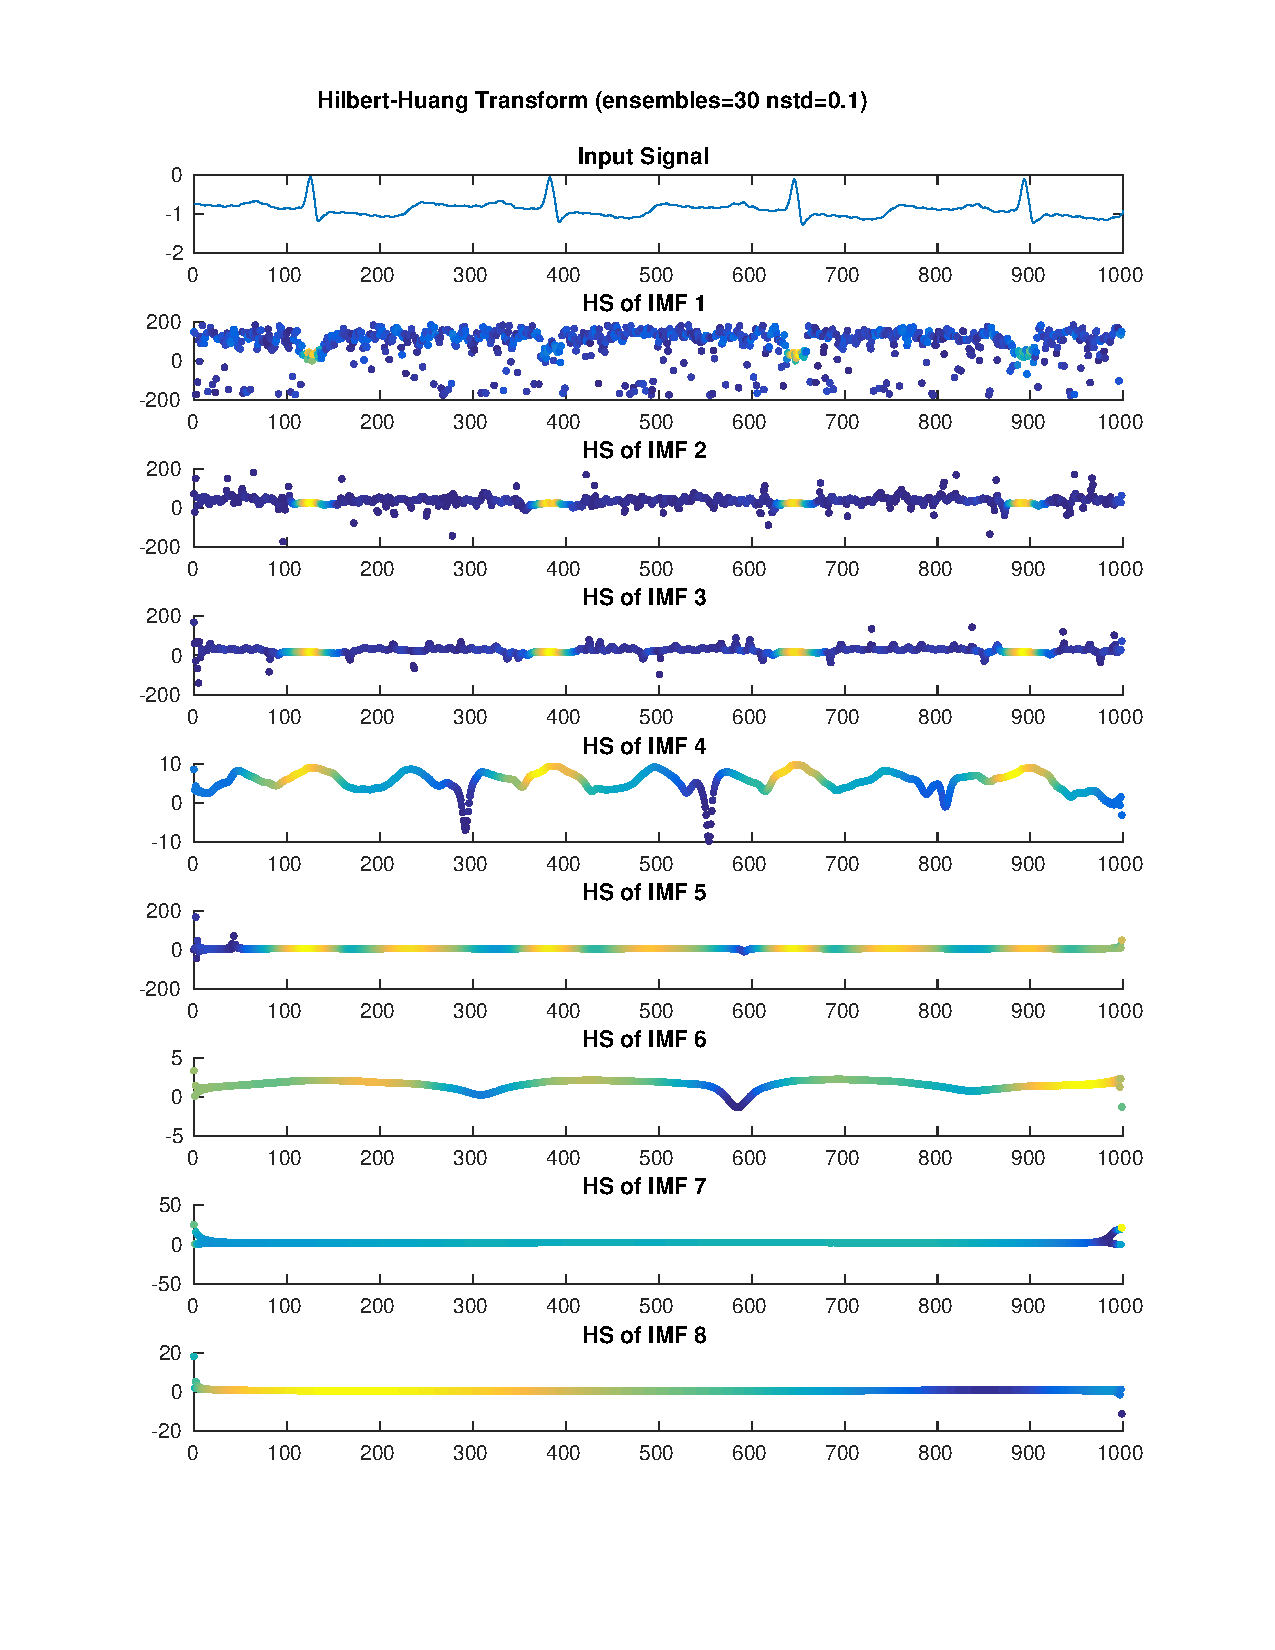
\includegraphics[width=\textwidth]{fig/112l1_hht_ensemble.pdf}
	
	(β)
\end{minipage}
\vfill
\caption{(α) Ensemble Emperical Mode Decomposition (β) Hilbert-Huang Transform του σήματος με $n_{ens}=50$ και $\sigma_n = 0.1$.}
\label{fig:112l1_hht_ensemble}
\end{figure}

\subsection*{112 (lead 2)}

% --- STFT, WDF, CWT ---
\begin{figure}[H]
\centering
\begin{minipage}{0.48\textwidth}
	\centering
	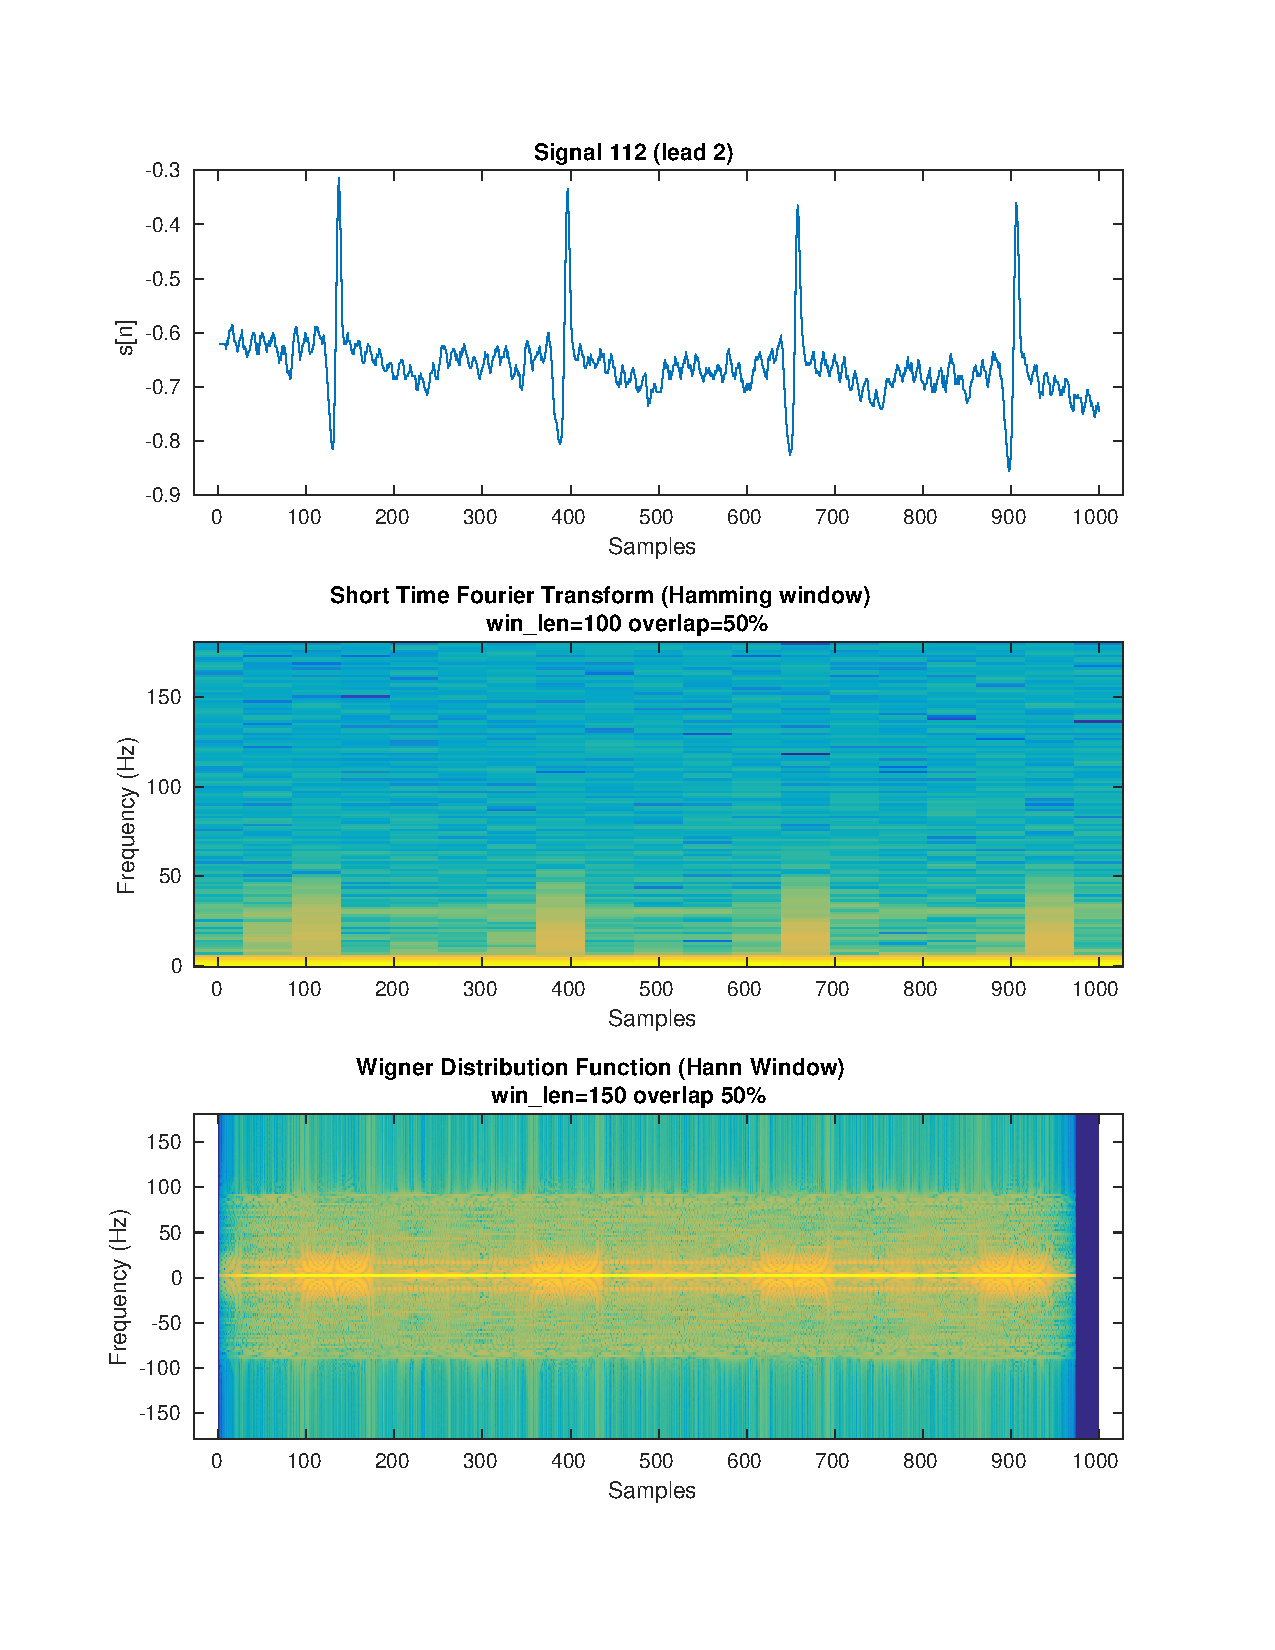
\includegraphics[width=\textwidth]{fig/112l2_stft_wdf.pdf}
	
	(α)
\end{minipage}
\begin{minipage}{0.48\textwidth}
	\centering
	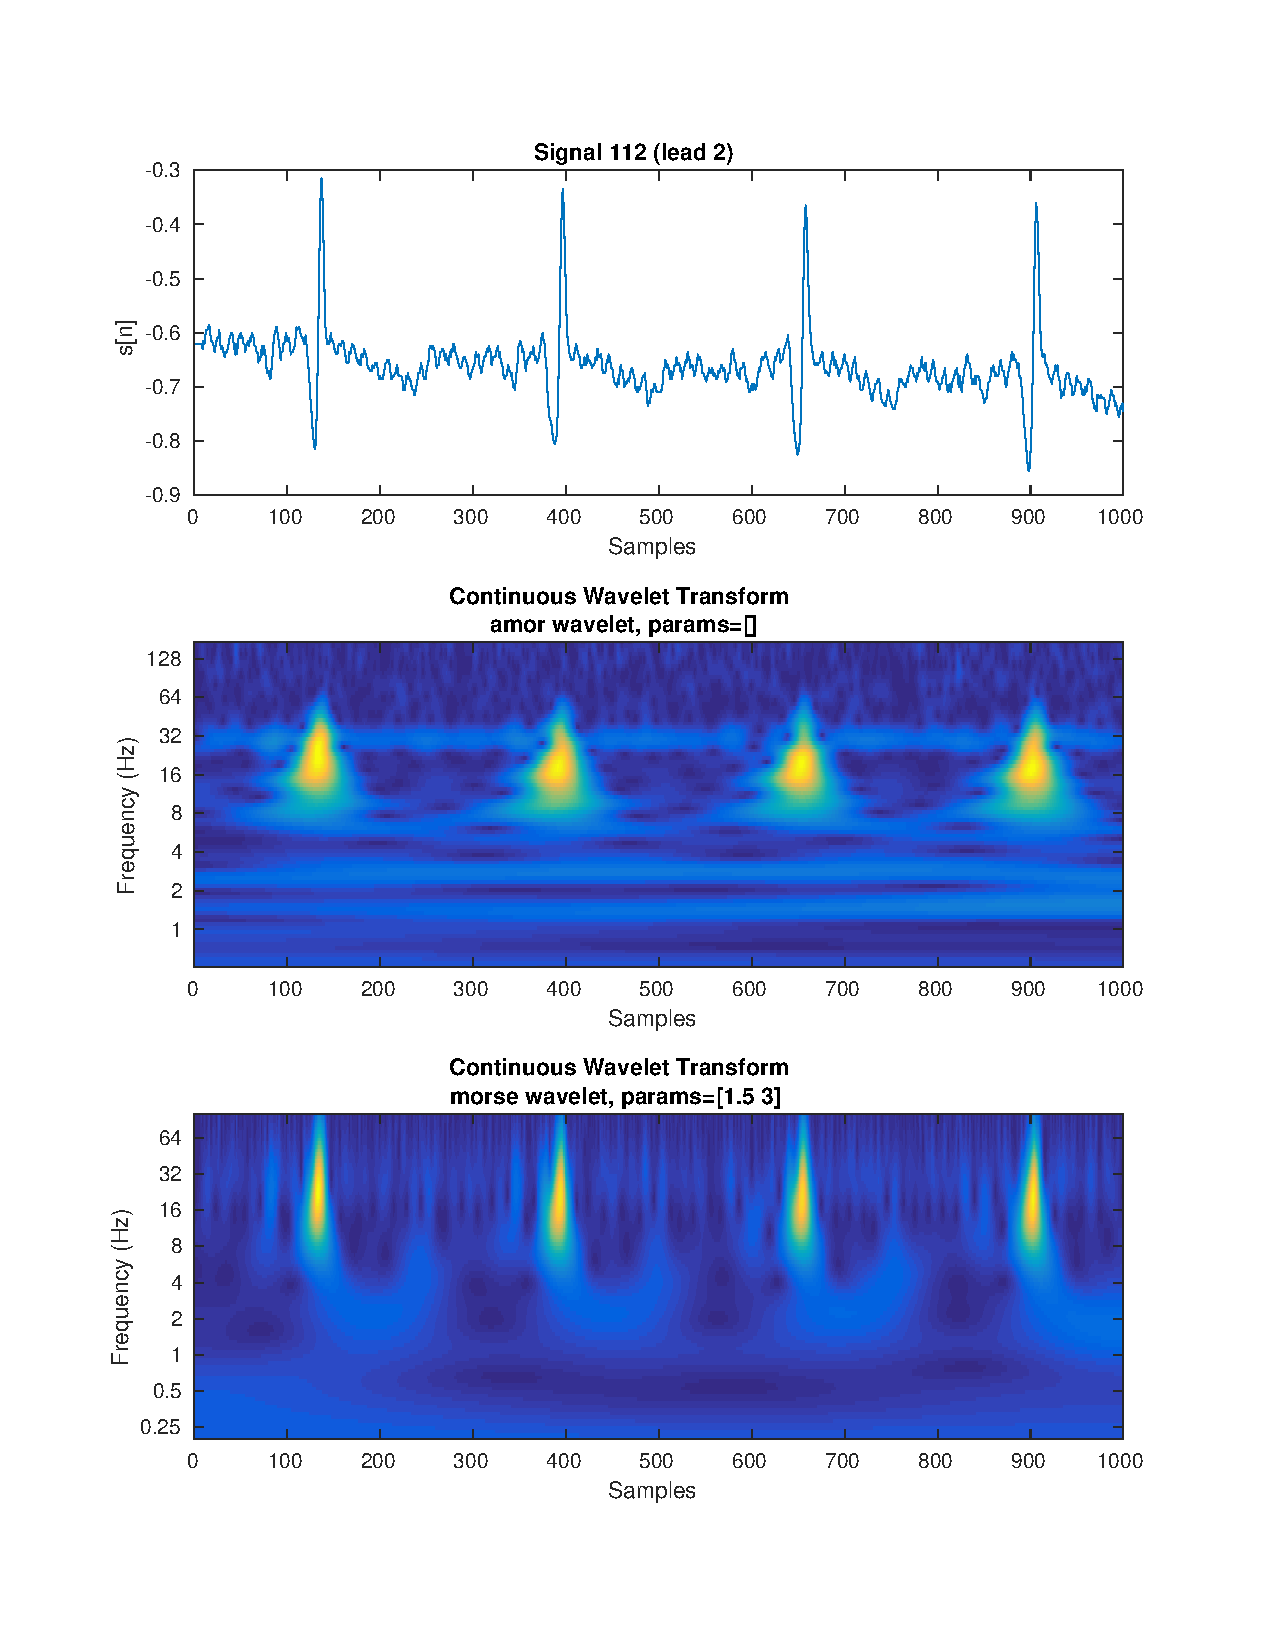
\includegraphics[width=\textwidth]{fig/112l2_cwt.pdf}
	
	(β)
\end{minipage}
\vfill
\caption{(α) Short Time Fourier Transform και Wigner Distribution Function (β) Wavelet Transform (Morlet, Morse wavelets) του σήματος.}
\label{fig:112l2_stft_wdf_wt}
\end{figure}


% --- DWT ---
\begin{figure}[H]
\centering
\begin{minipage}{0.48\textwidth}
	\centering
	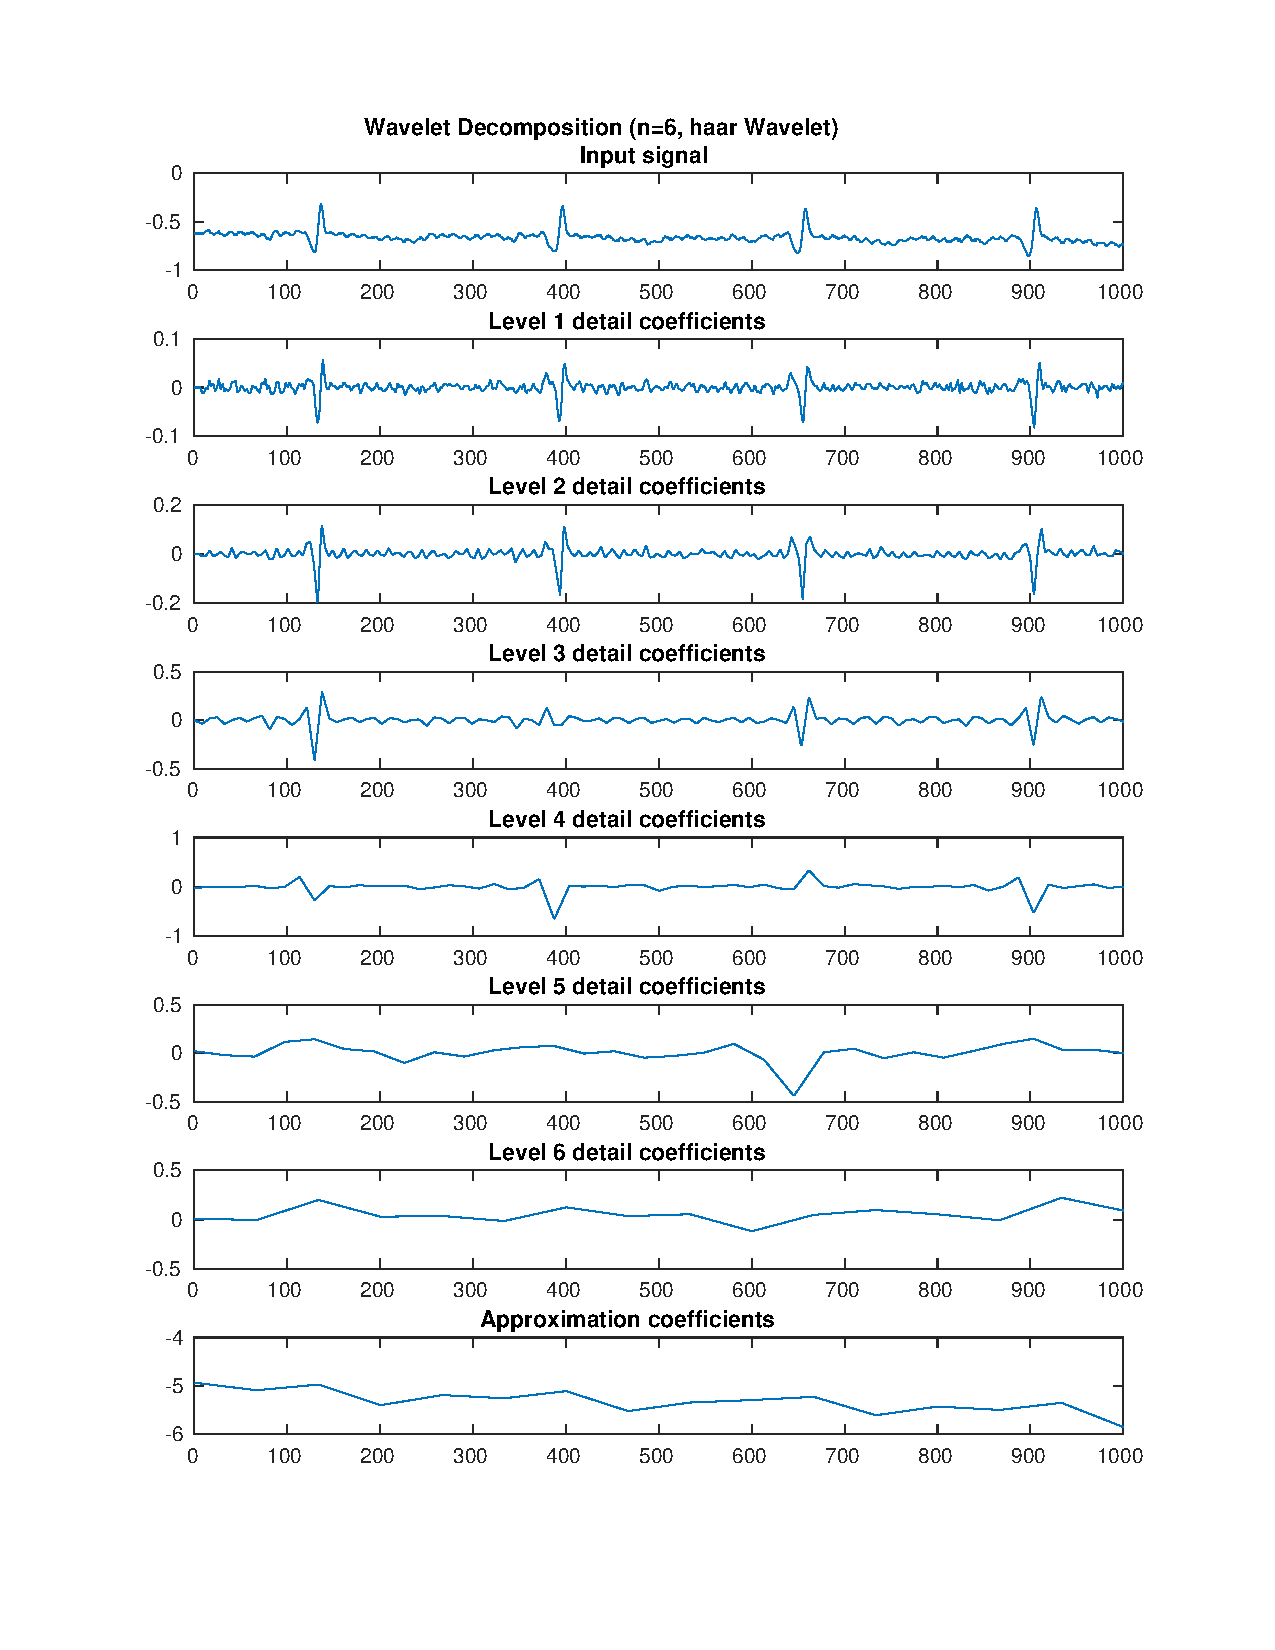
\includegraphics[width=\textwidth]{fig/112l2_dwt1.pdf}
	
	(α)
\end{minipage}
\begin{minipage}{0.48\textwidth}
	\centering
	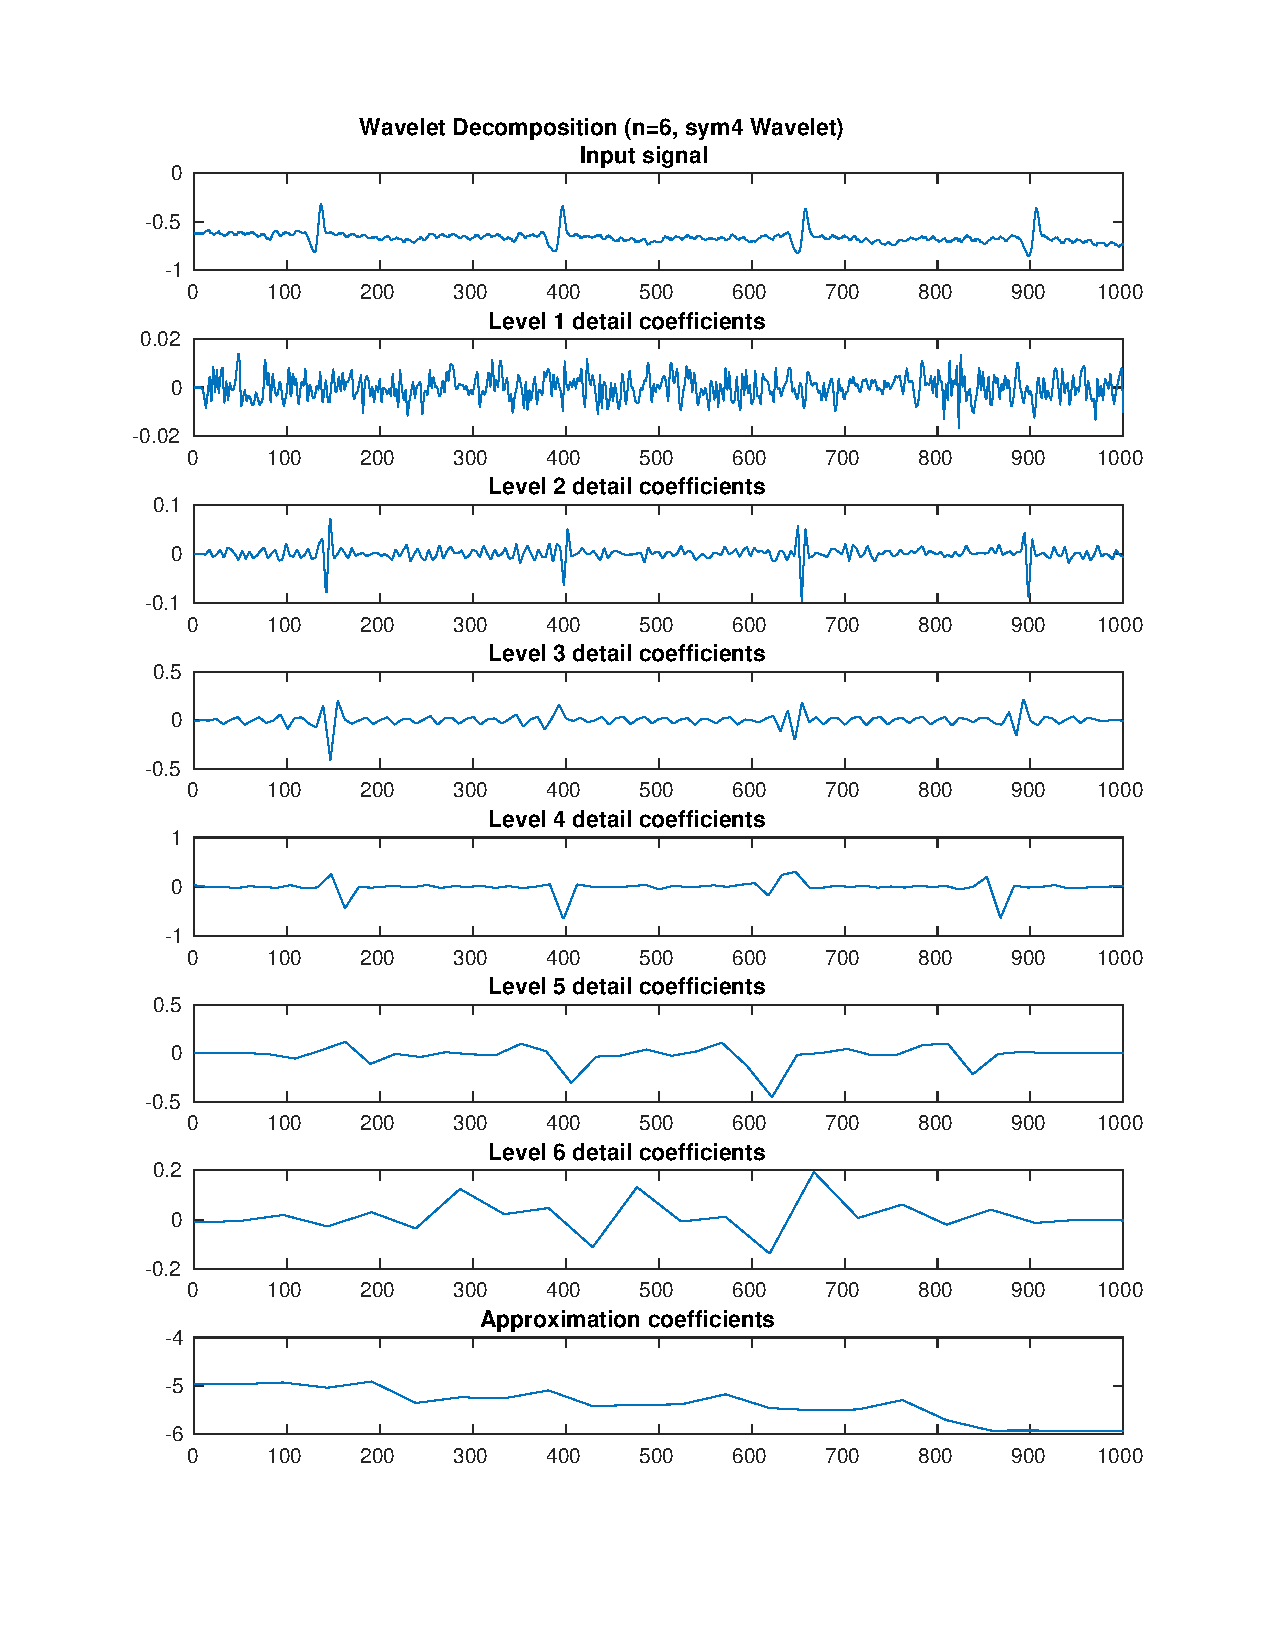
\includegraphics[width=\textwidth]{fig/112l2_dwt2.pdf}
	
	(β)
\end{minipage}
\vfill
\caption{Wavelet Decomposition του σήματος χρησιμοποιώντας wavelet (α) Haar (β) Symlet4.}
\label{fig:112l2_dwt}
\end{figure}


% --- EMD/HHT ---
\begin{figure}[H]
\centering
\begin{minipage}{0.48\textwidth}
	\centering
	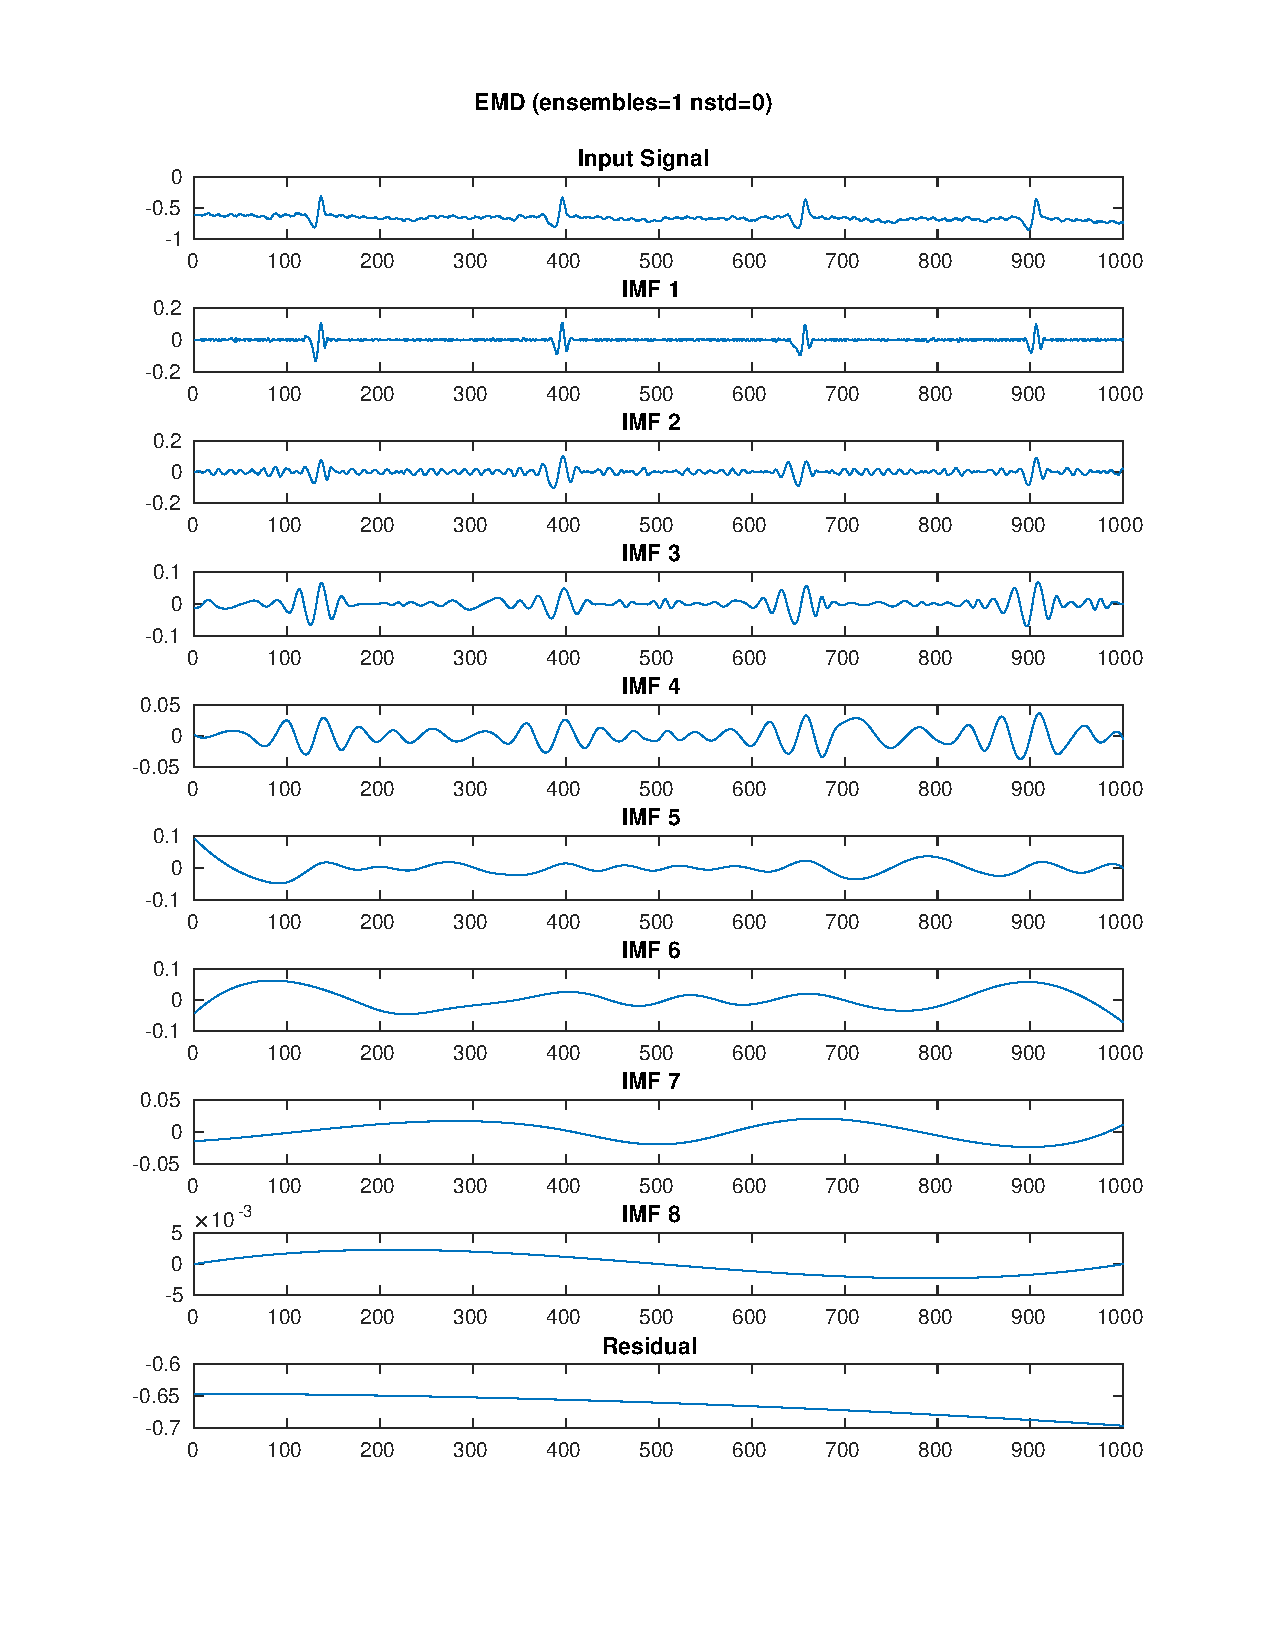
\includegraphics[width=\textwidth]{fig/112l2_emd.pdf}
	
	(α)
\end{minipage}
\begin{minipage}{0.48\textwidth}
	\centering
	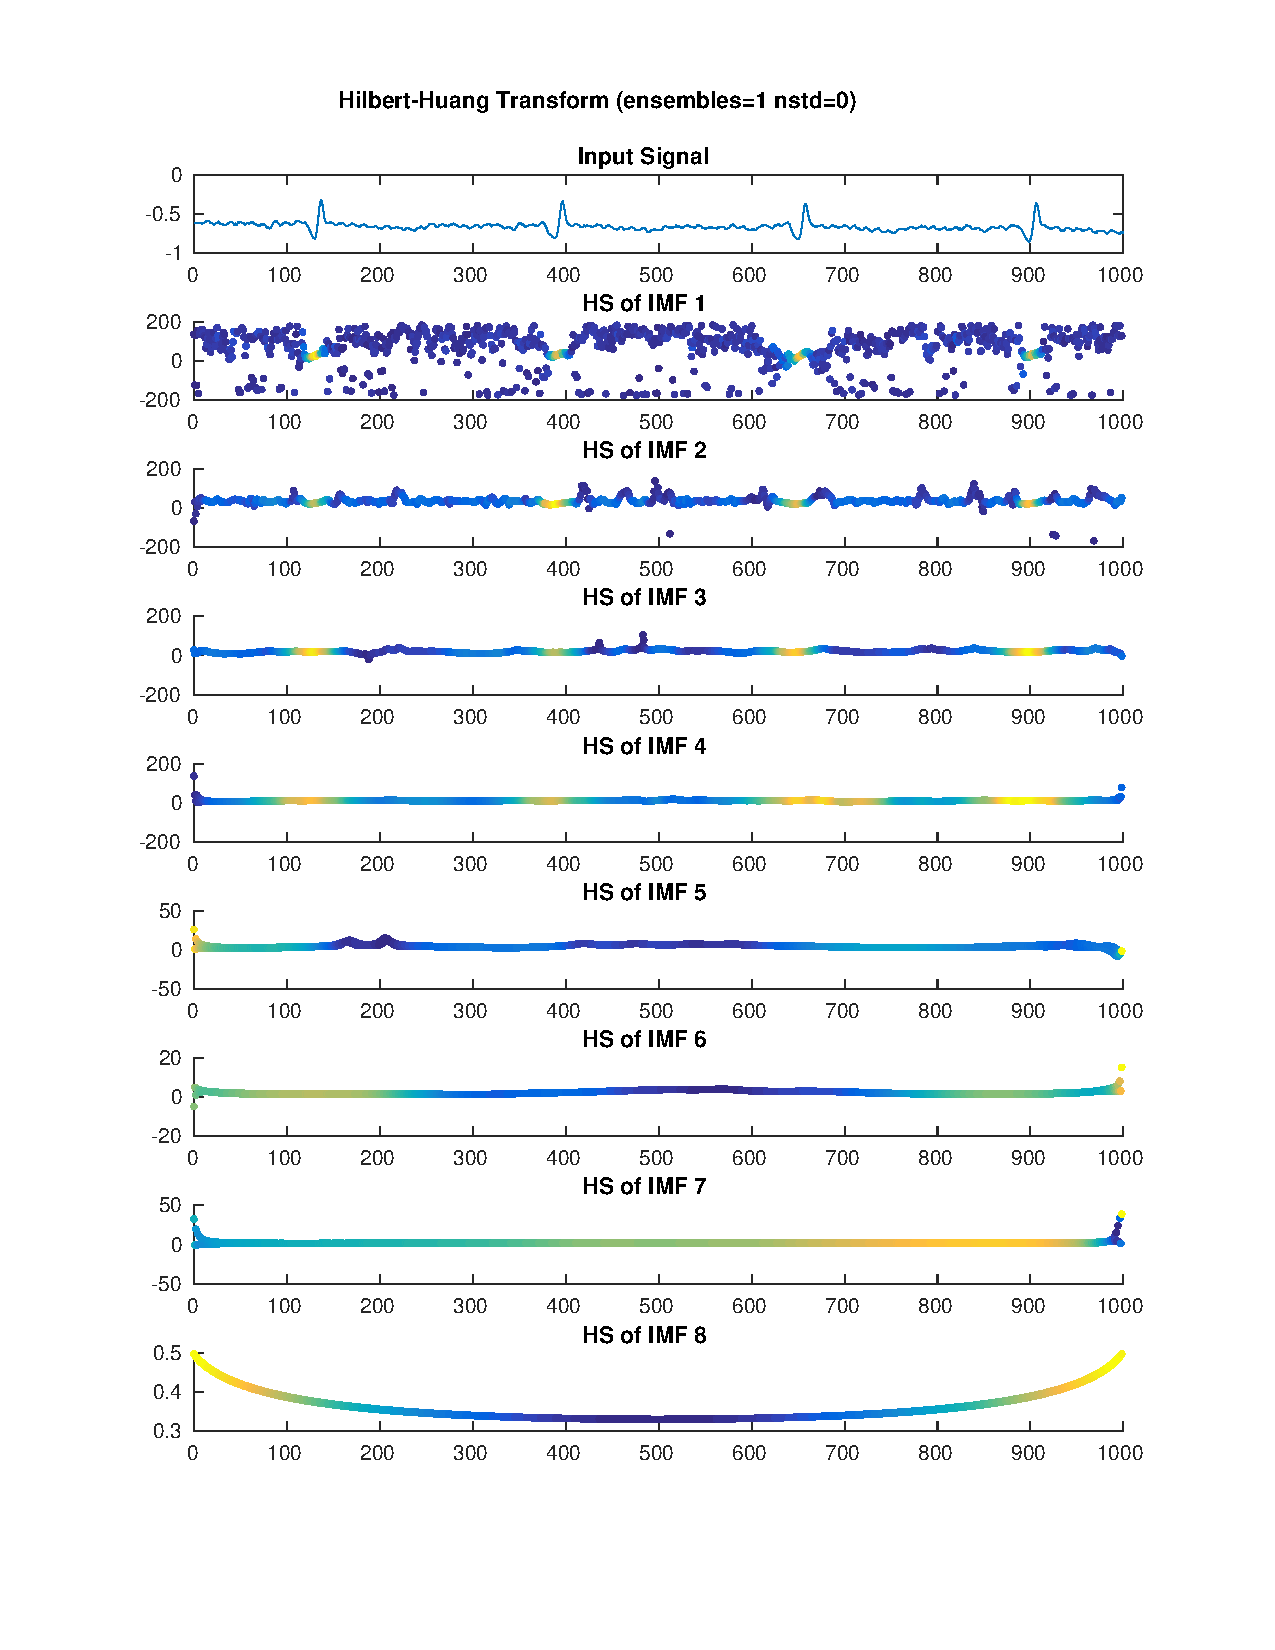
\includegraphics[width=\textwidth]{fig/112l2_hht.pdf}
	
	(β)
\end{minipage}
\vfill
\caption{(α) Emperical Mode Decomposition (β) Hilbert-Huang Transform του σήματος.}
\label{fig:112l2_hht}
\end{figure}


% --- EEMD/HHT ---
\begin{figure}[H]
\centering
\begin{minipage}{0.48\textwidth}
	\centering
	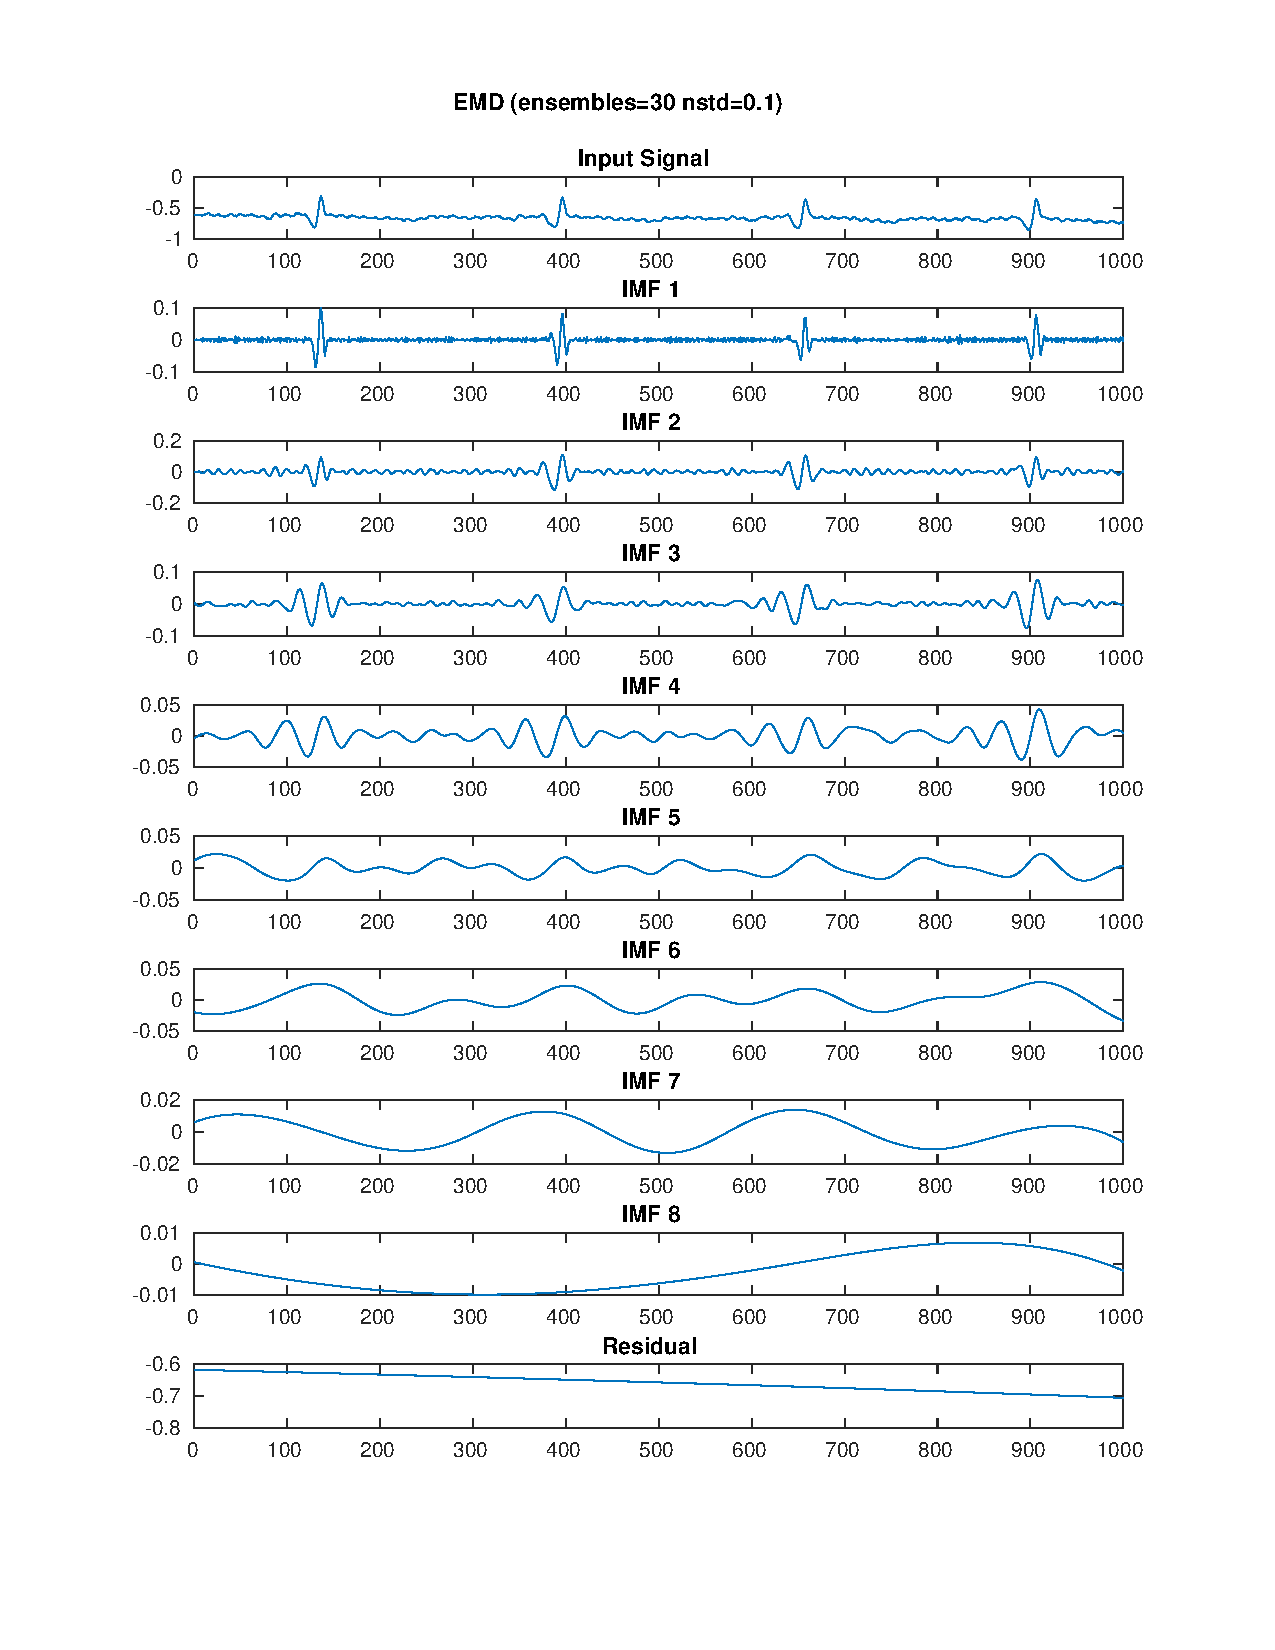
\includegraphics[width=\textwidth]{fig/112l2_emd_ensemble.pdf}
	
	(α)
\end{minipage}
\begin{minipage}{0.48\textwidth}
	\centering
	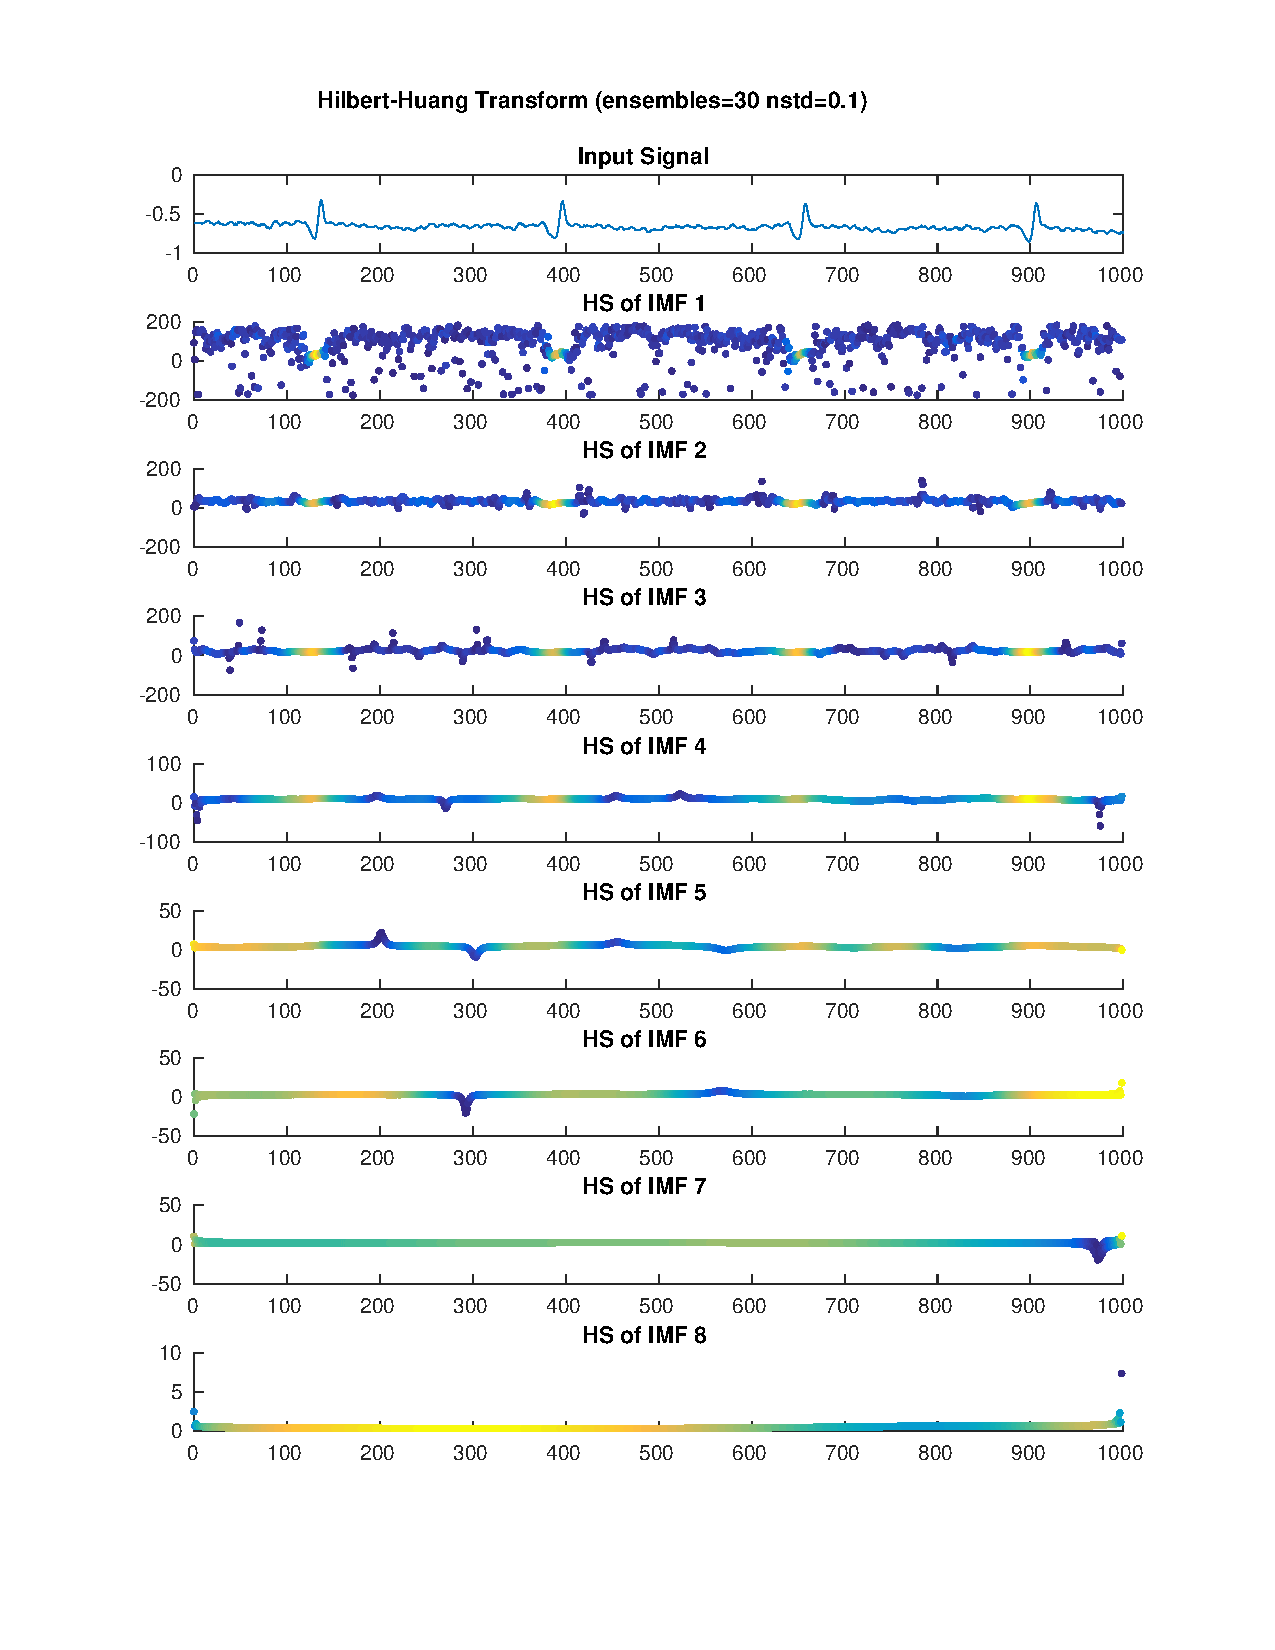
\includegraphics[width=\textwidth]{fig/112l2_hht_ensemble.pdf}
	
	(β)
\end{minipage}
\vfill
\caption{(α) Ensemble Emperical Mode Decomposition (β) Hilbert-Huang Transform του σήματος με $n_{ens}=50$ και $\sigma_n = 0.1$.}
\label{fig:112l2_hht_ensemble}
\end{figure}


\subsection*{123}

% --- STFT, WDF, CWT ---
\begin{figure}[H]
\centering
\begin{minipage}{0.48\textwidth}
	\centering
	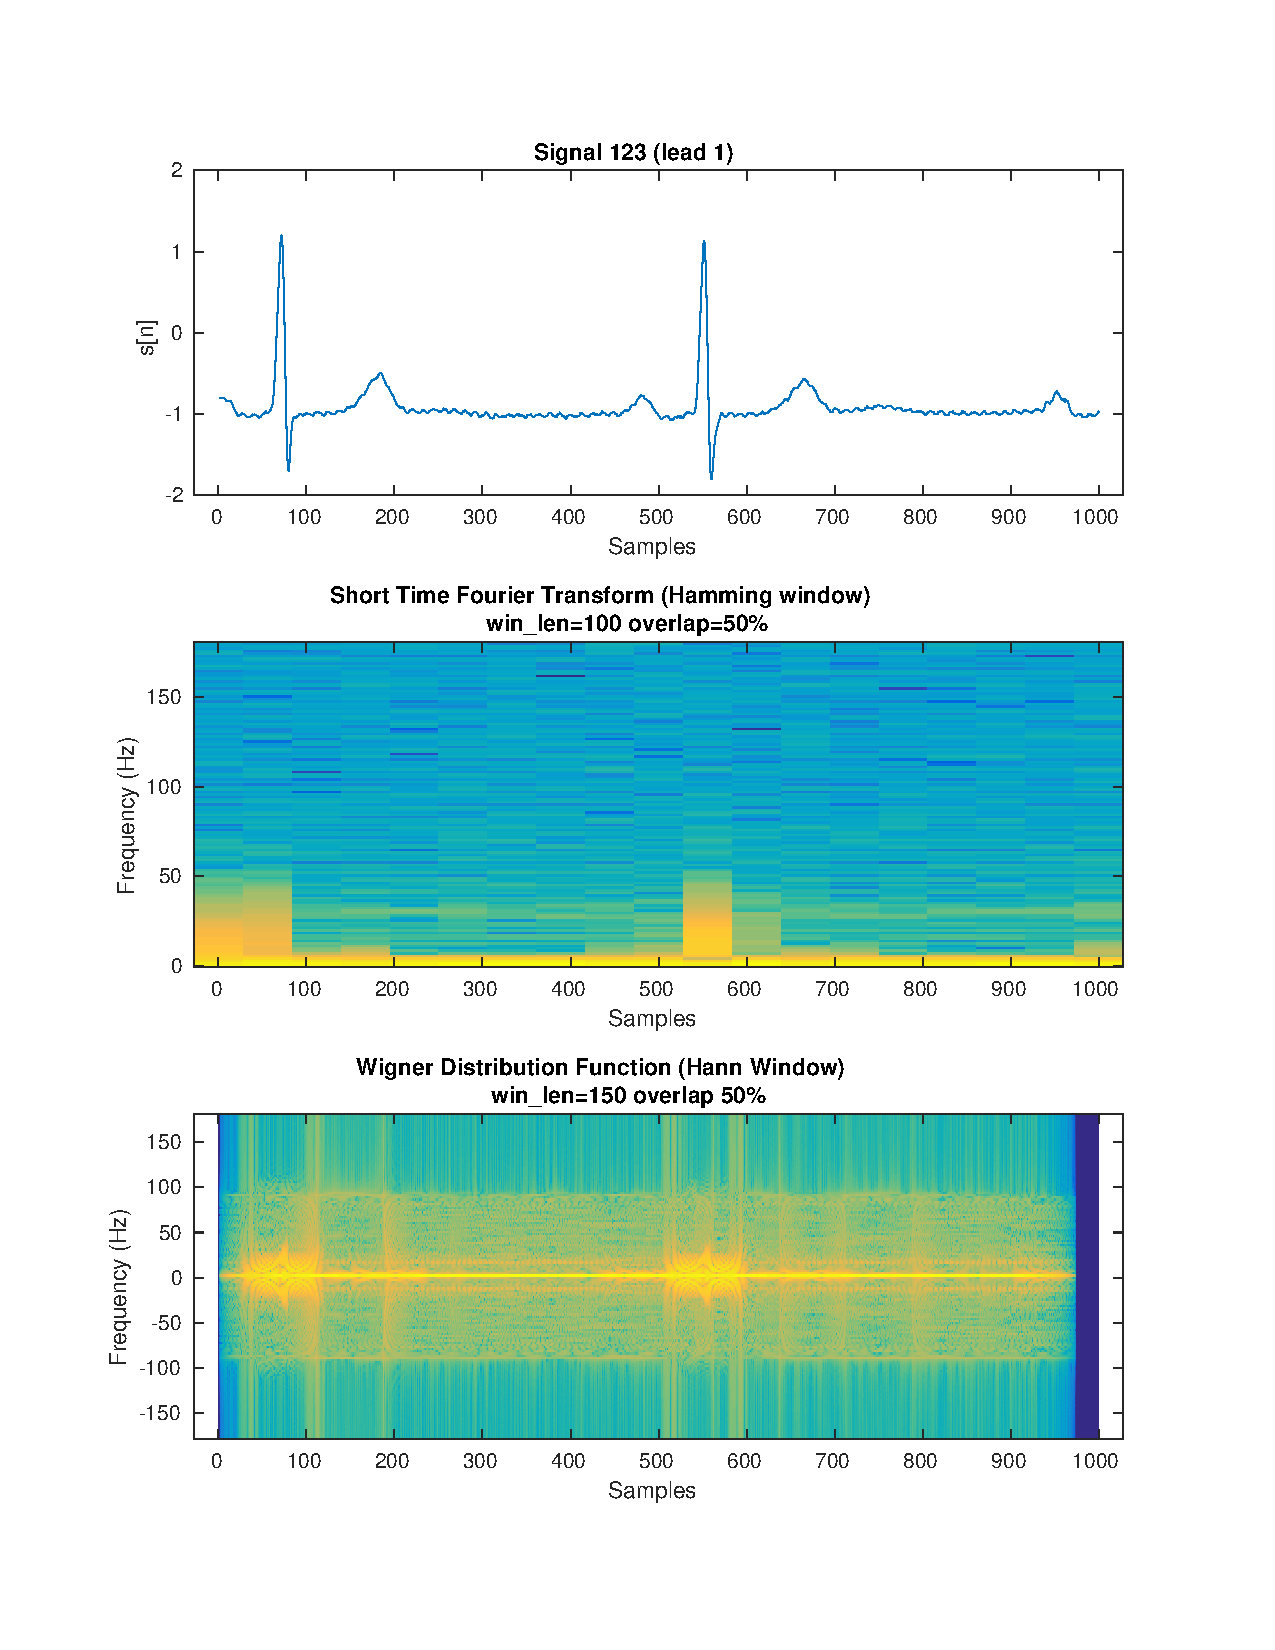
\includegraphics[width=\textwidth]{fig/123l1_stft_wdf.pdf}
	
	(α)
\end{minipage}
\begin{minipage}{0.48\textwidth}
	\centering
	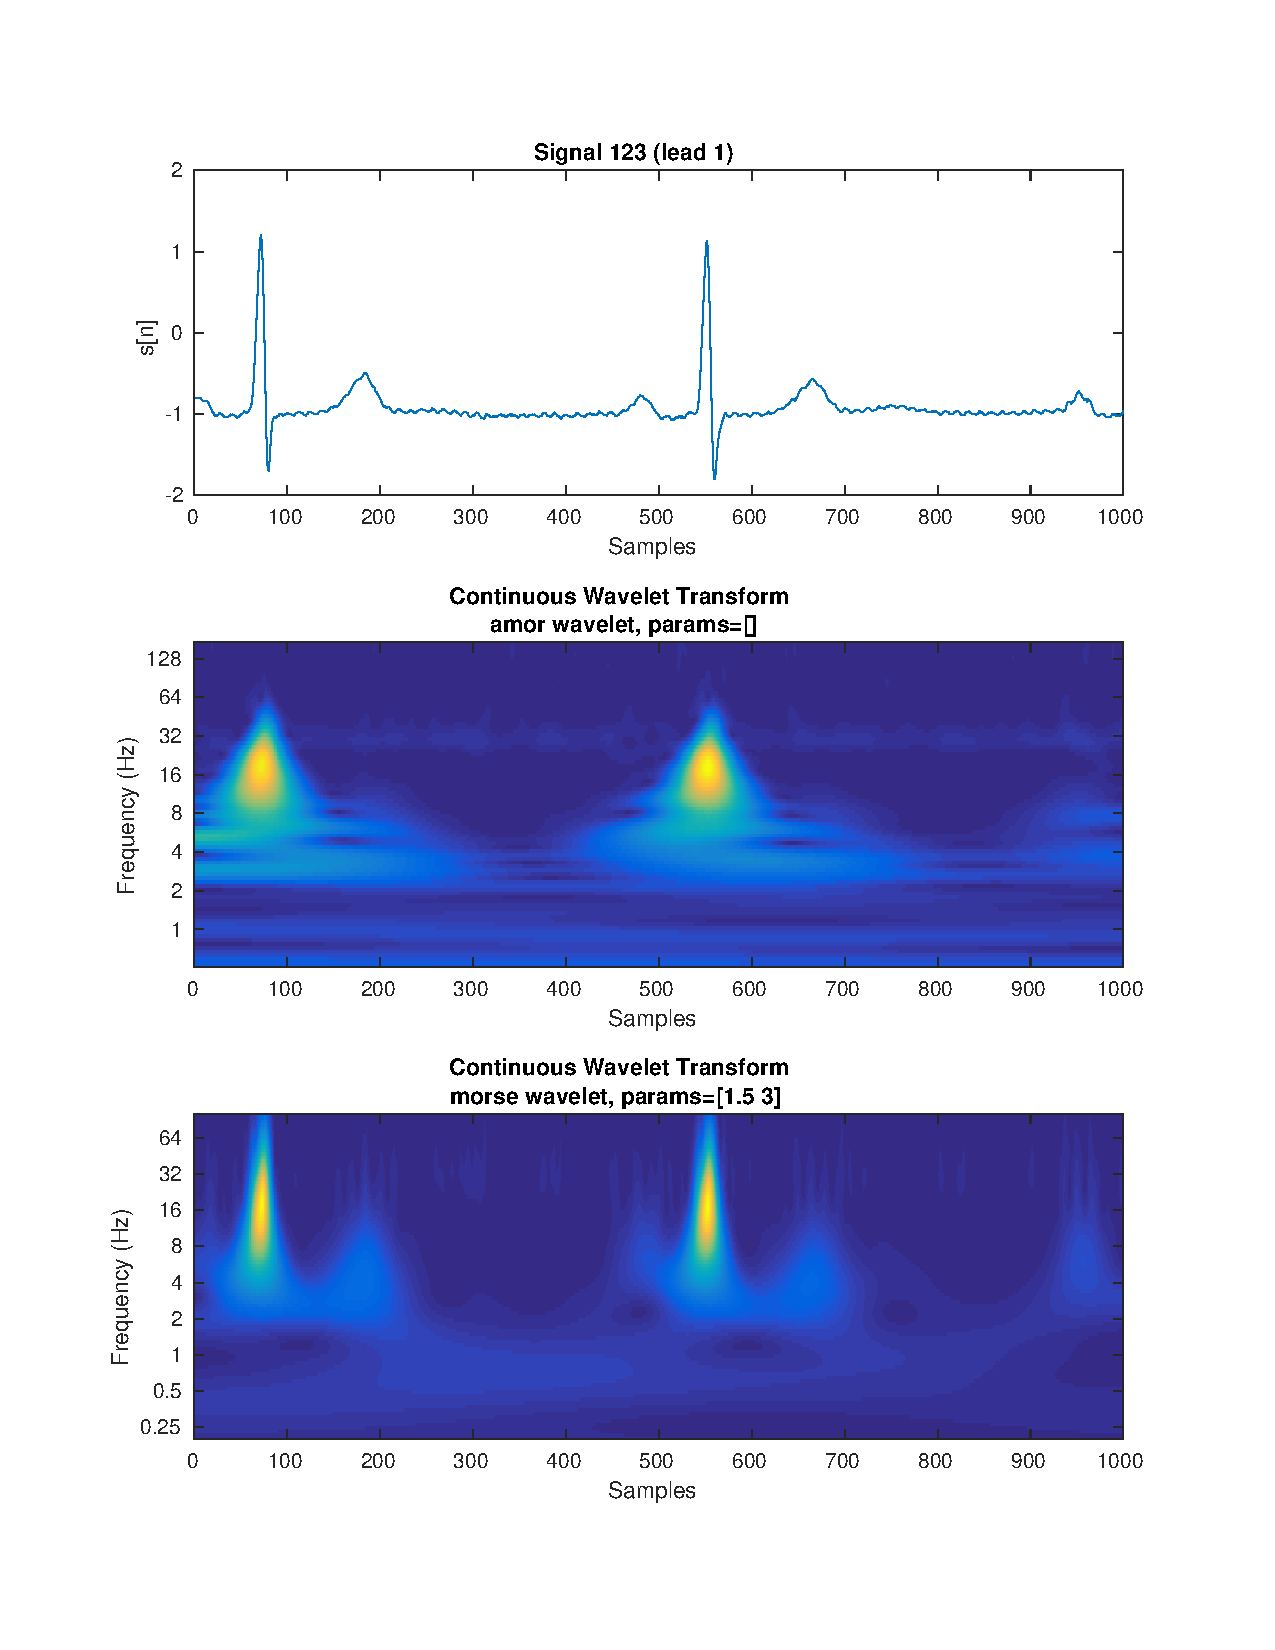
\includegraphics[width=\textwidth]{fig/123l1_cwt.pdf}
	
	(β)
\end{minipage}
\vfill
\caption{(α) Short Time Fourier Transform και Wigner Distribution Function (β) Wavelet Transform (Morlet, Morse wavelets) του σήματος.}
\label{fig:123l1_stft_wdf_wt}
\end{figure}


% --- DWT ---
\begin{figure}[H]
\centering
\begin{minipage}{0.48\textwidth}
	\centering
	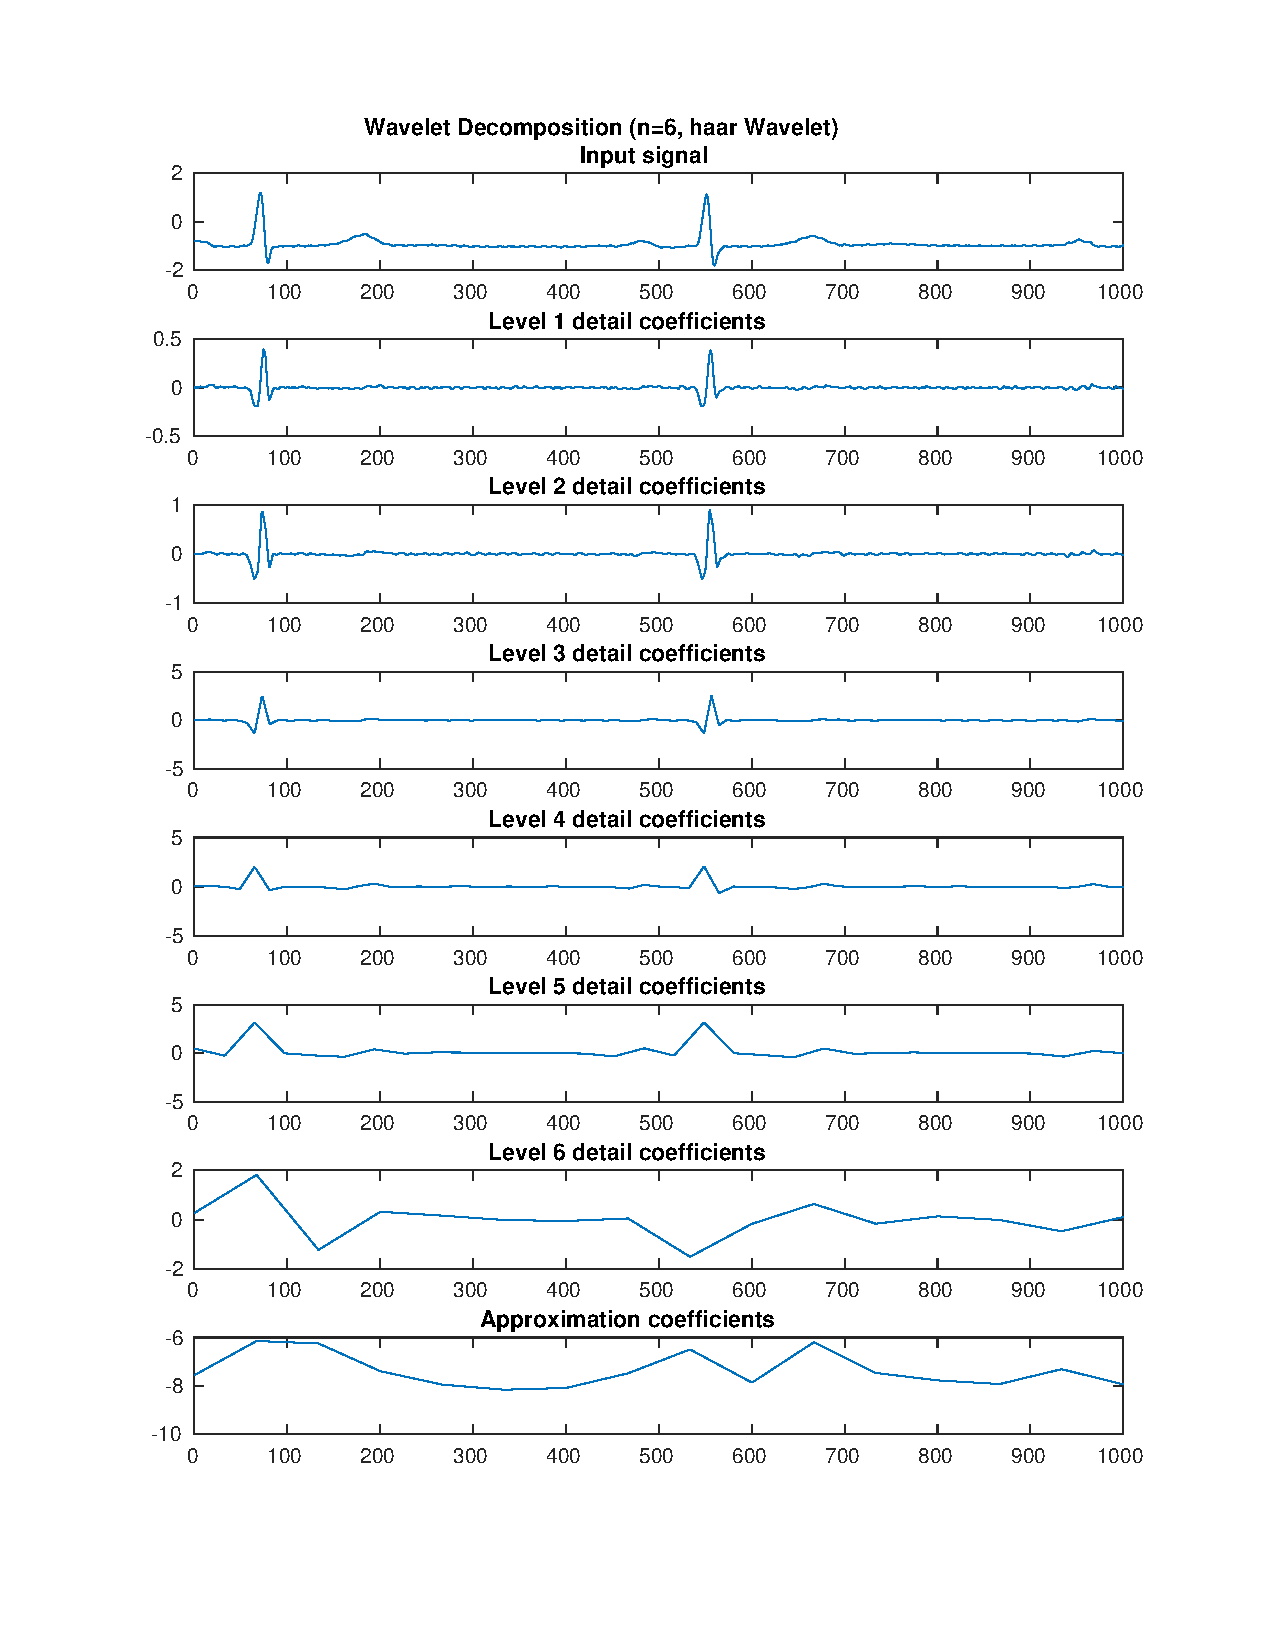
\includegraphics[width=\textwidth]{fig/123l1_dwt1.pdf}
	
	(α)
\end{minipage}
\begin{minipage}{0.48\textwidth}
	\centering
	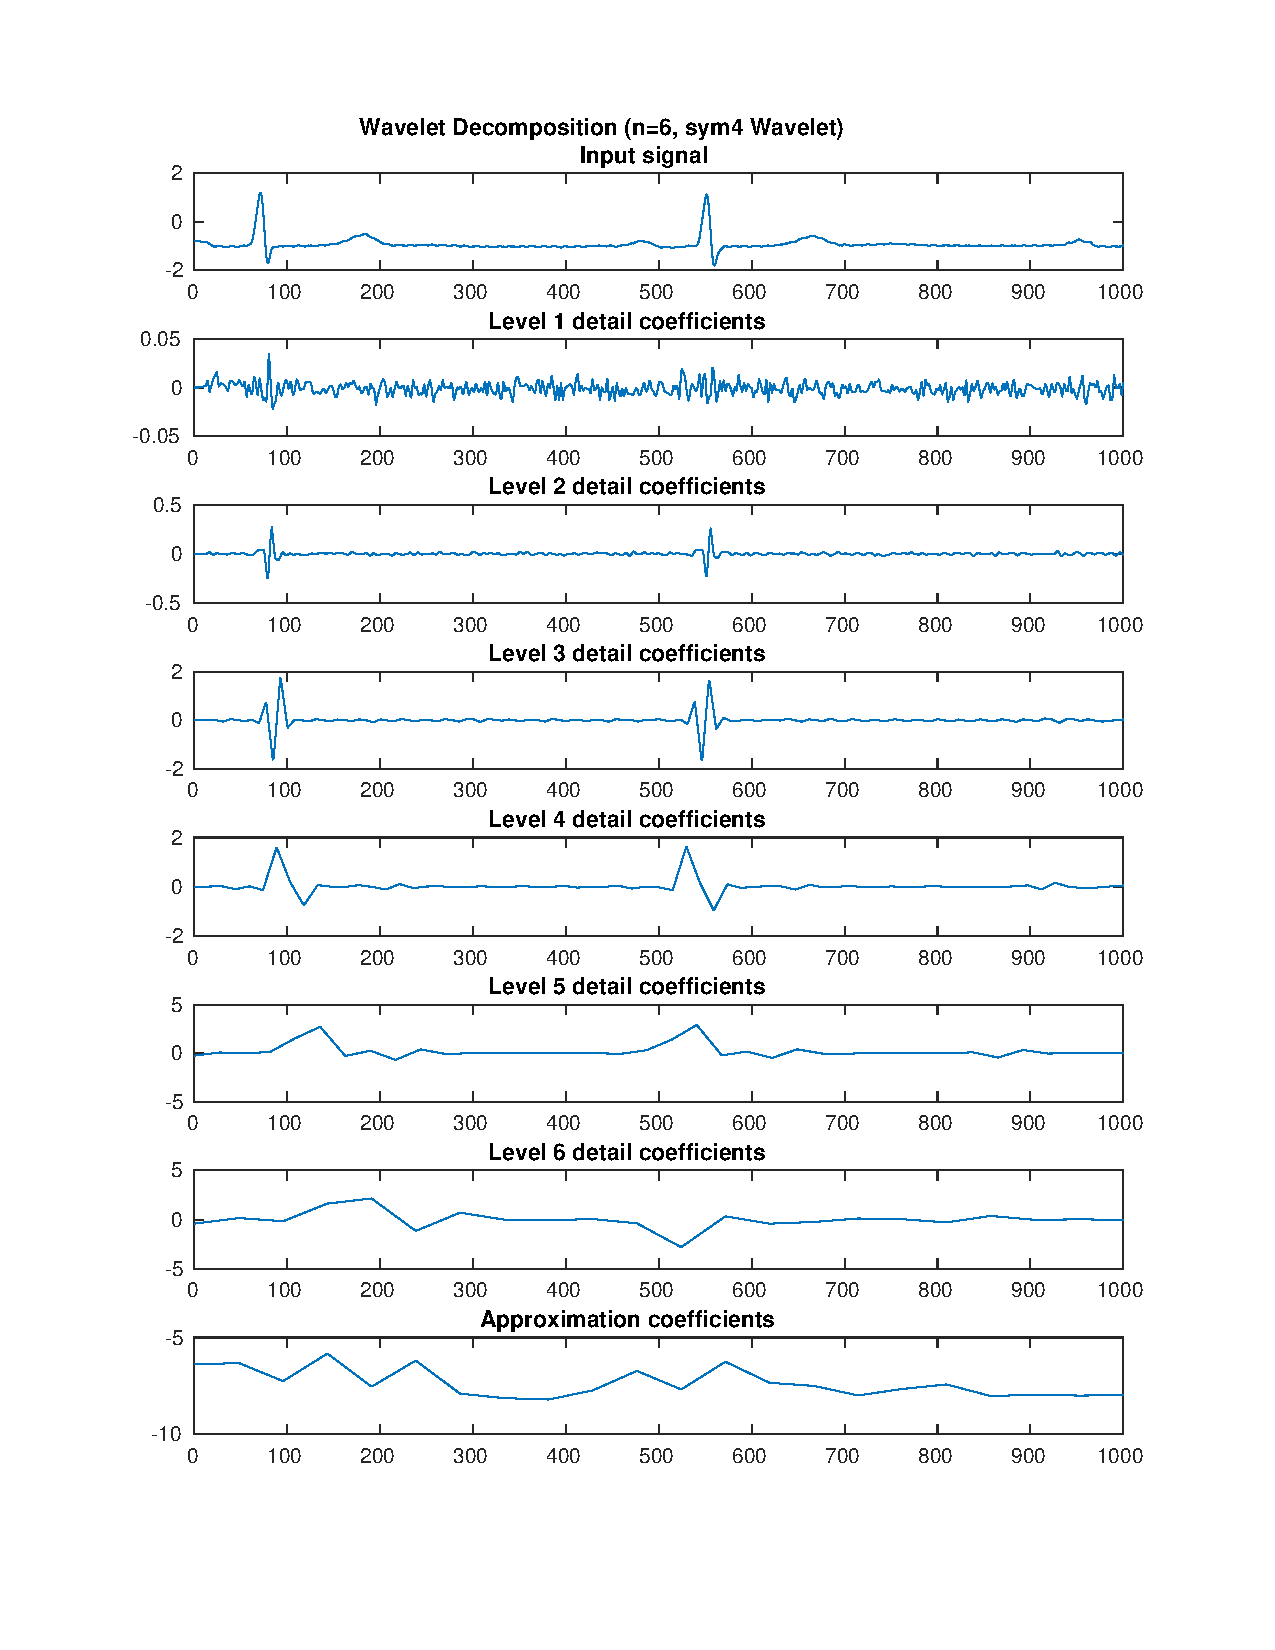
\includegraphics[width=\textwidth]{fig/123l1_dwt2.pdf}
	
	(β)
\end{minipage}
\vfill
\caption{Wavelet Decomposition του σήματος χρησιμοποιώντας wavelet (α) Haar (β) Symlet4.}
\label{fig:123l1_dwt}
\end{figure}


% --- EMD/HHT ---
\begin{figure}[H]
\centering
\begin{minipage}{0.48\textwidth}
	\centering
	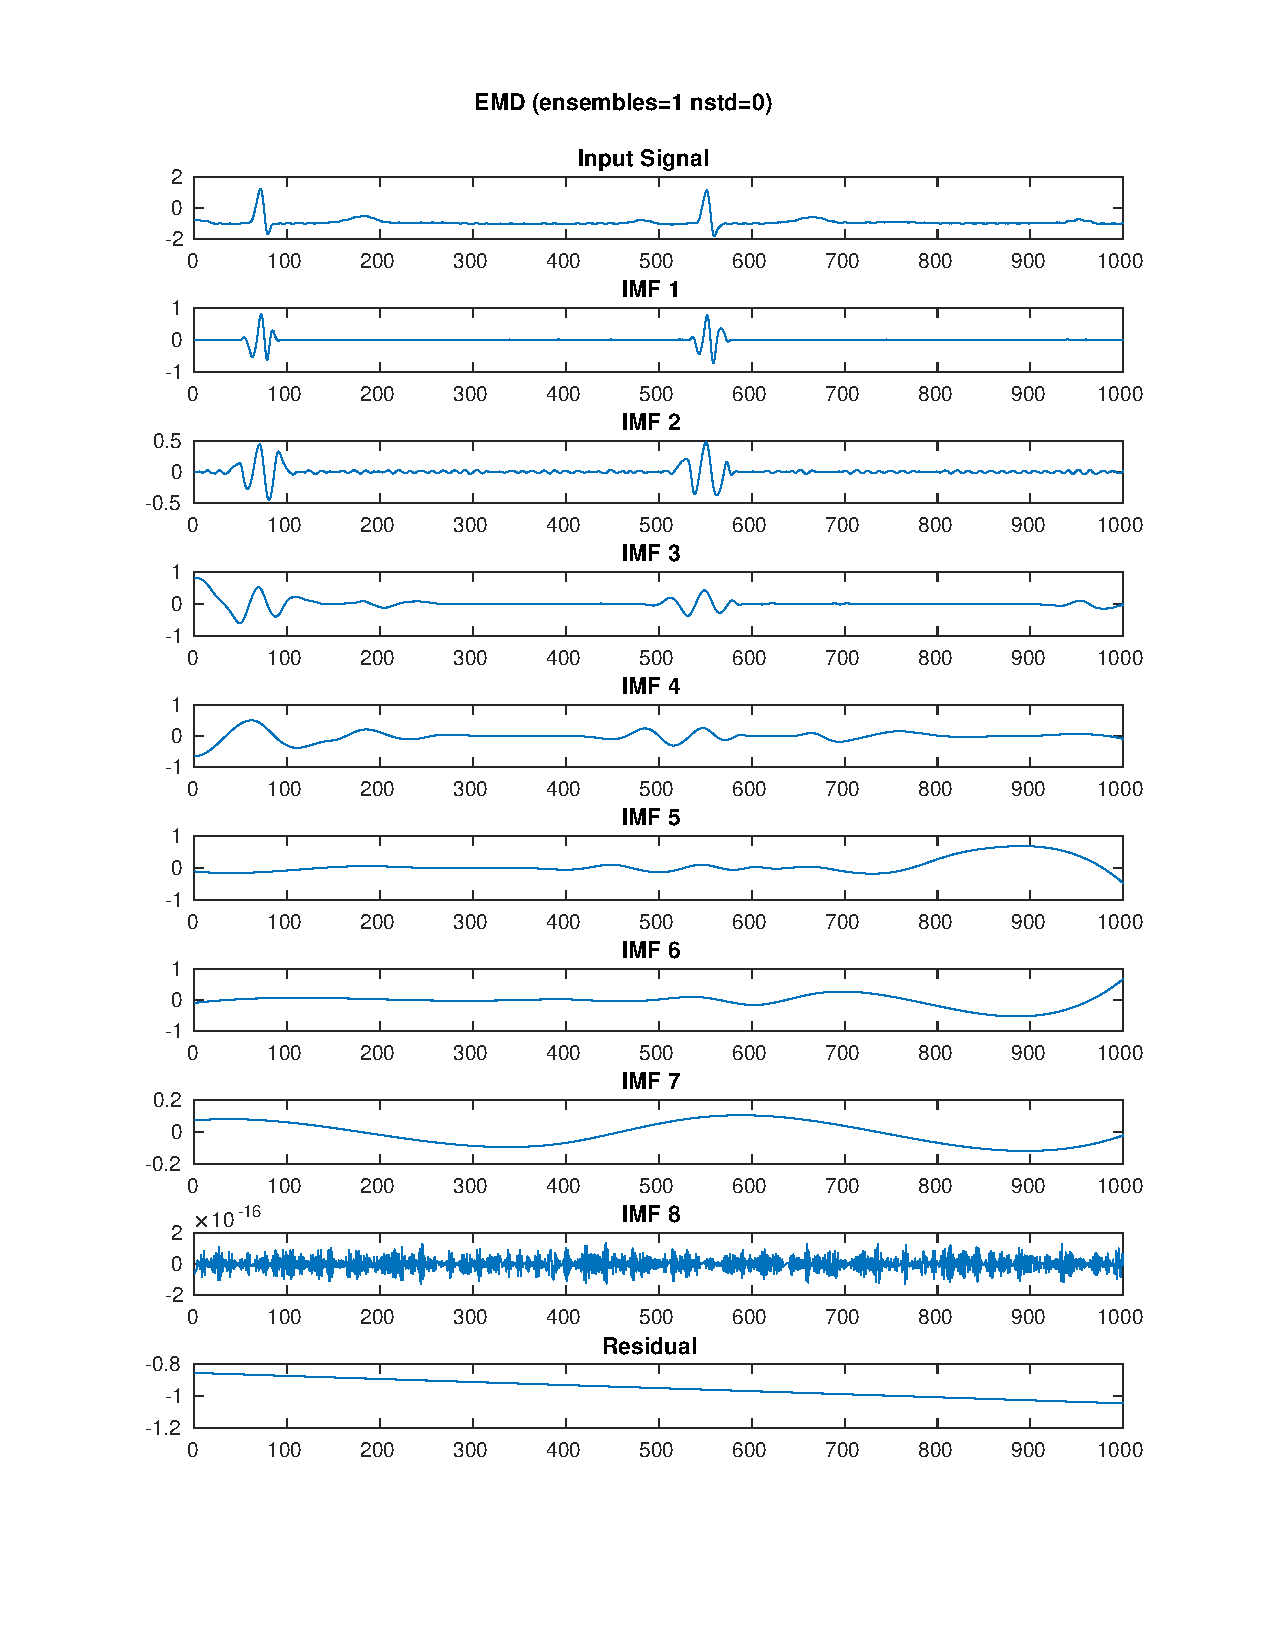
\includegraphics[width=\textwidth]{fig/123l1_emd.pdf}
	
	(α)
\end{minipage}
\begin{minipage}{0.48\textwidth}
	\centering
	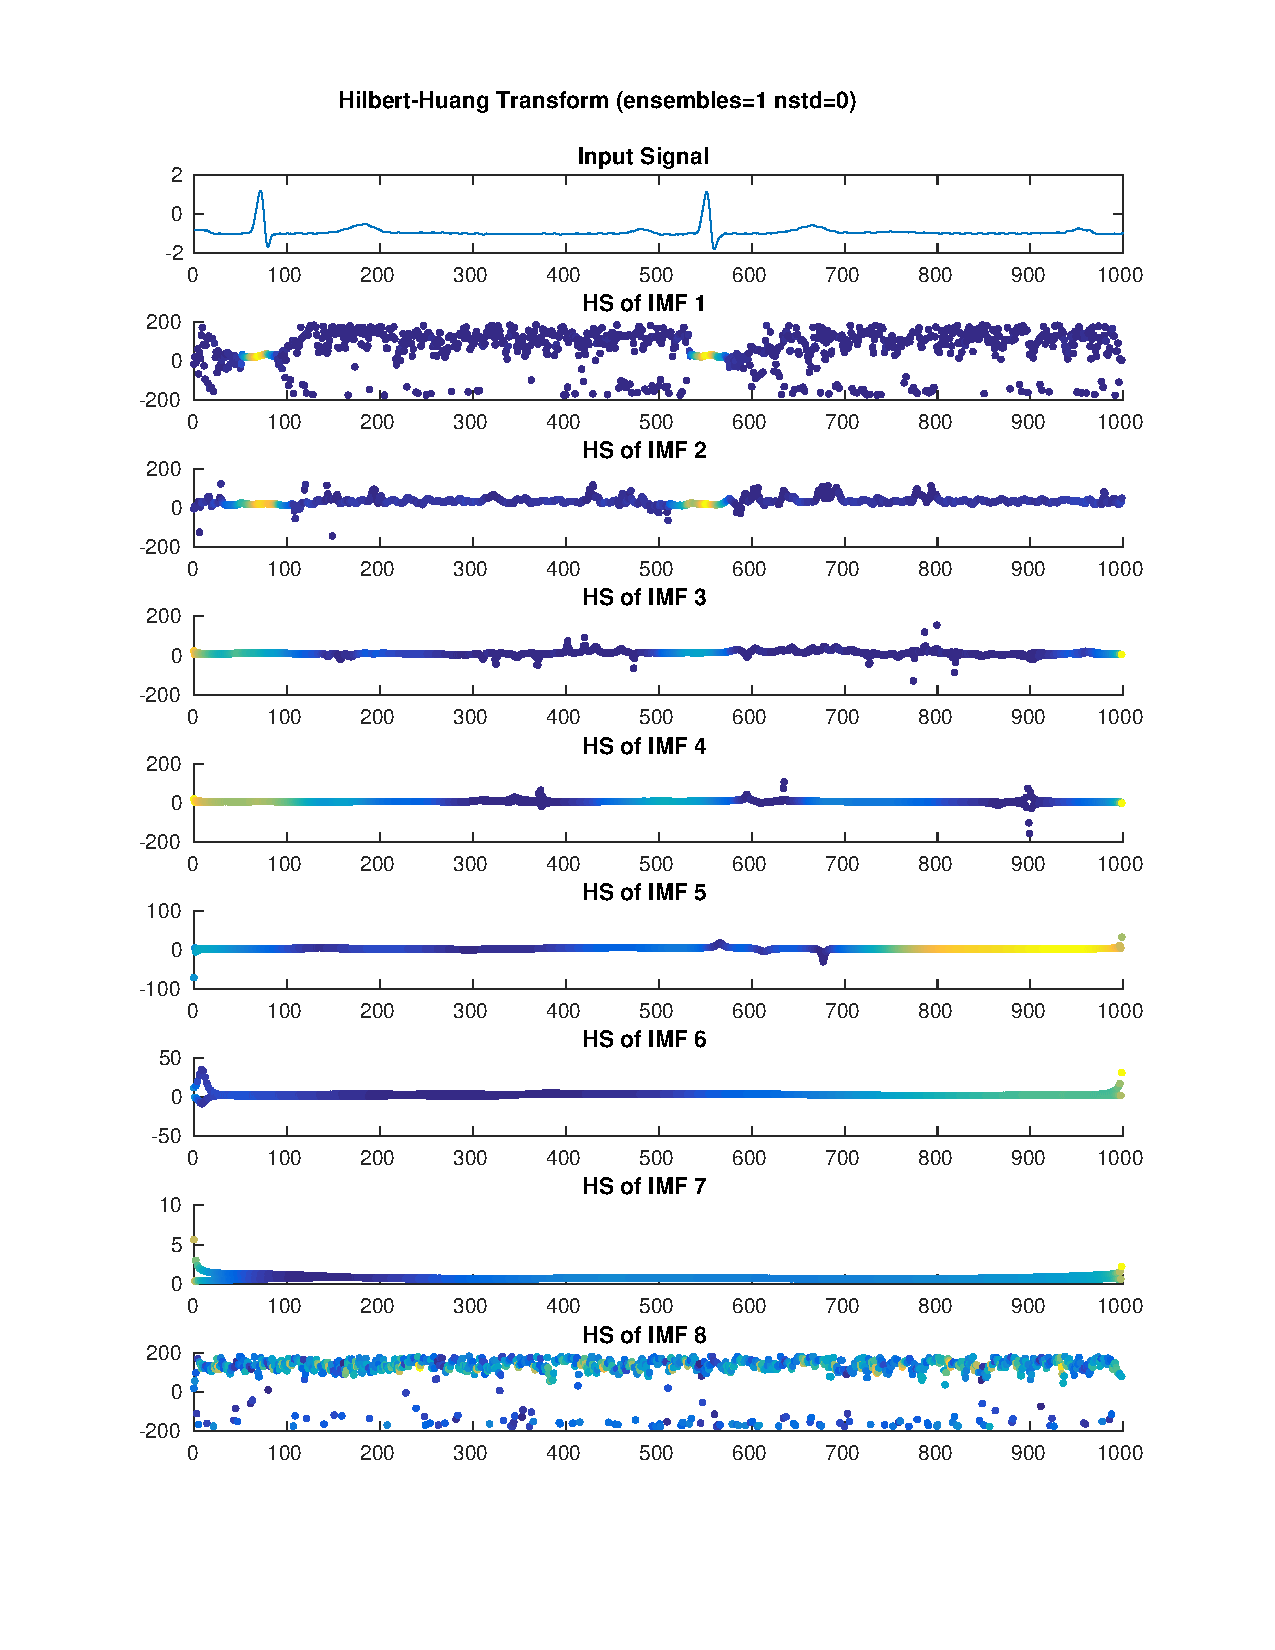
\includegraphics[width=\textwidth]{fig/123l1_hht.pdf}
	
	(β)
\end{minipage}
\vfill
\caption{(α) Emperical Mode Decomposition (β) Hilbert-Huang Transform του σήματος.}
\label{fig:123l1_hht}
\end{figure}


% --- EEMD/HHT ---
\begin{figure}[H]
\centering
\begin{minipage}{0.48\textwidth}
	\centering
	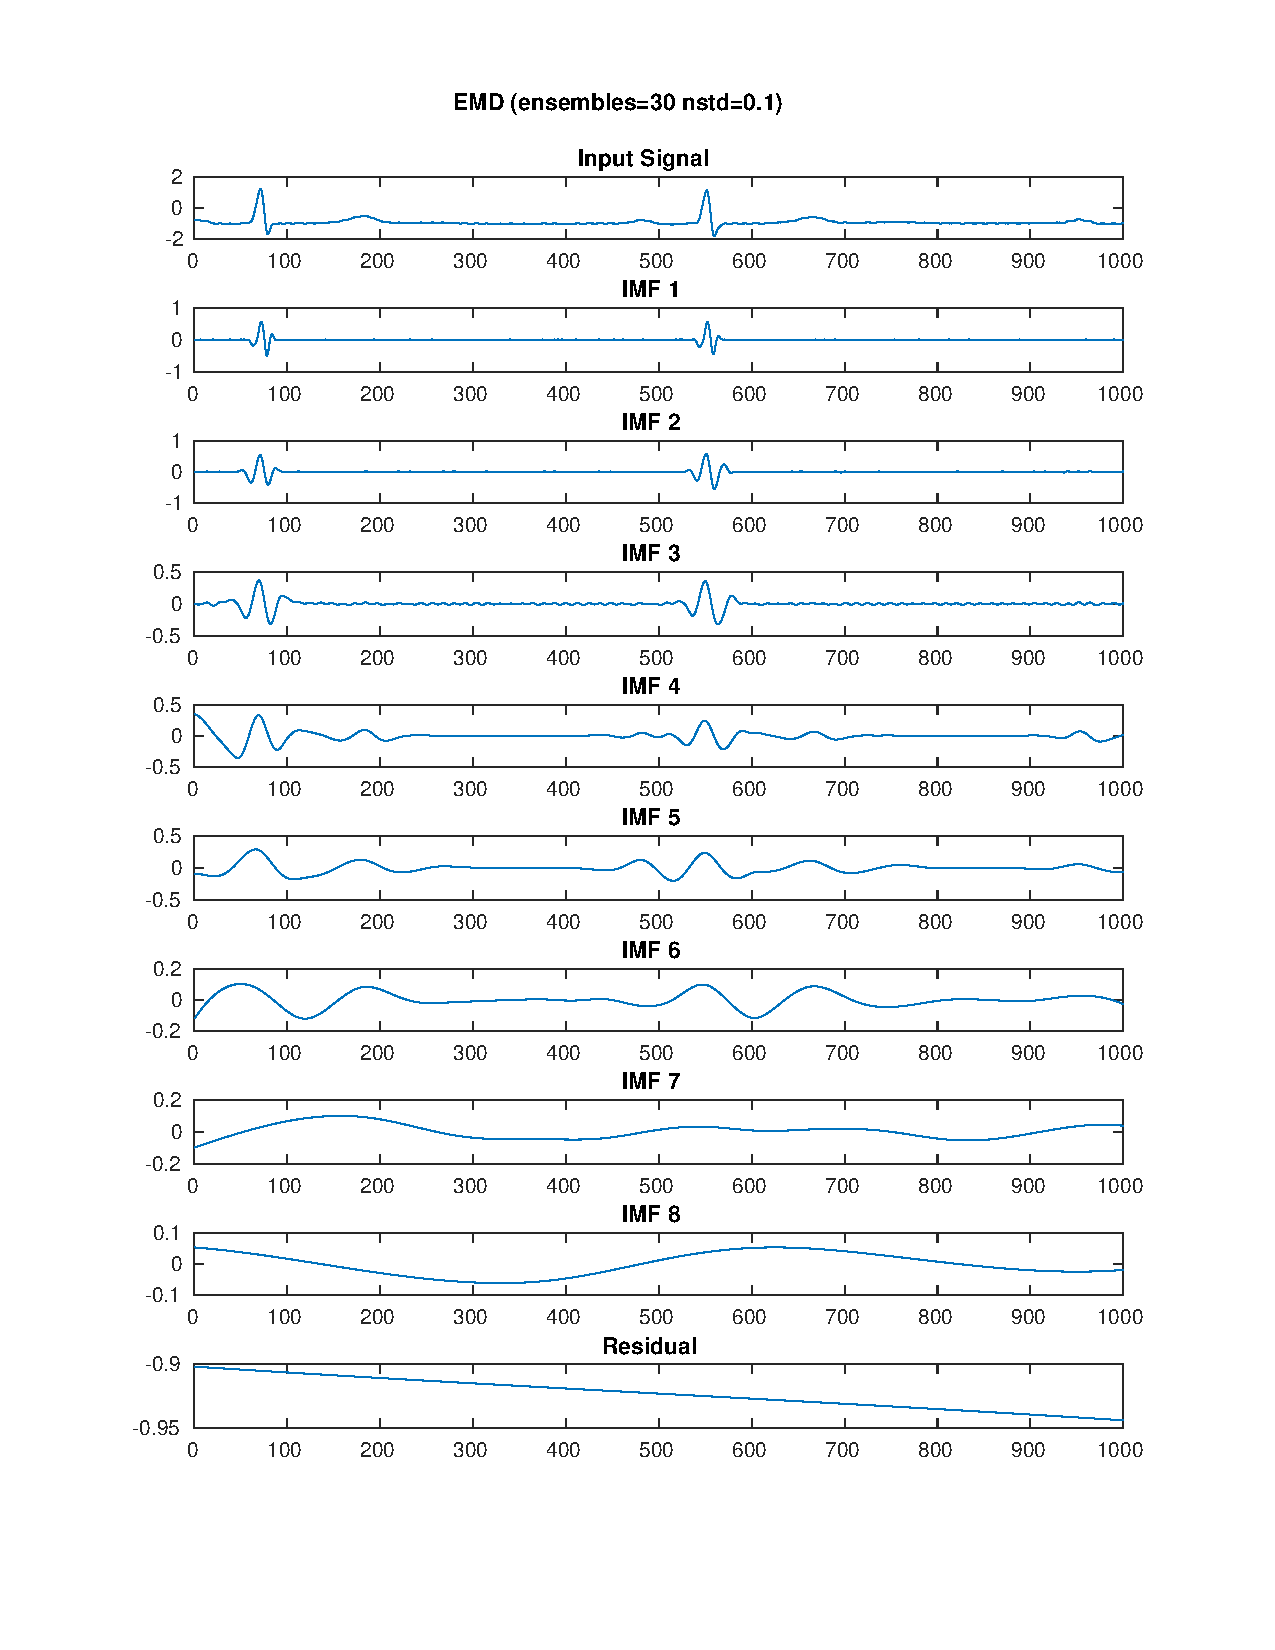
\includegraphics[width=\textwidth]{fig/123l1_emd_ensemble.pdf}
	
	(α)
\end{minipage}
\begin{minipage}{0.48\textwidth}
	\centering
	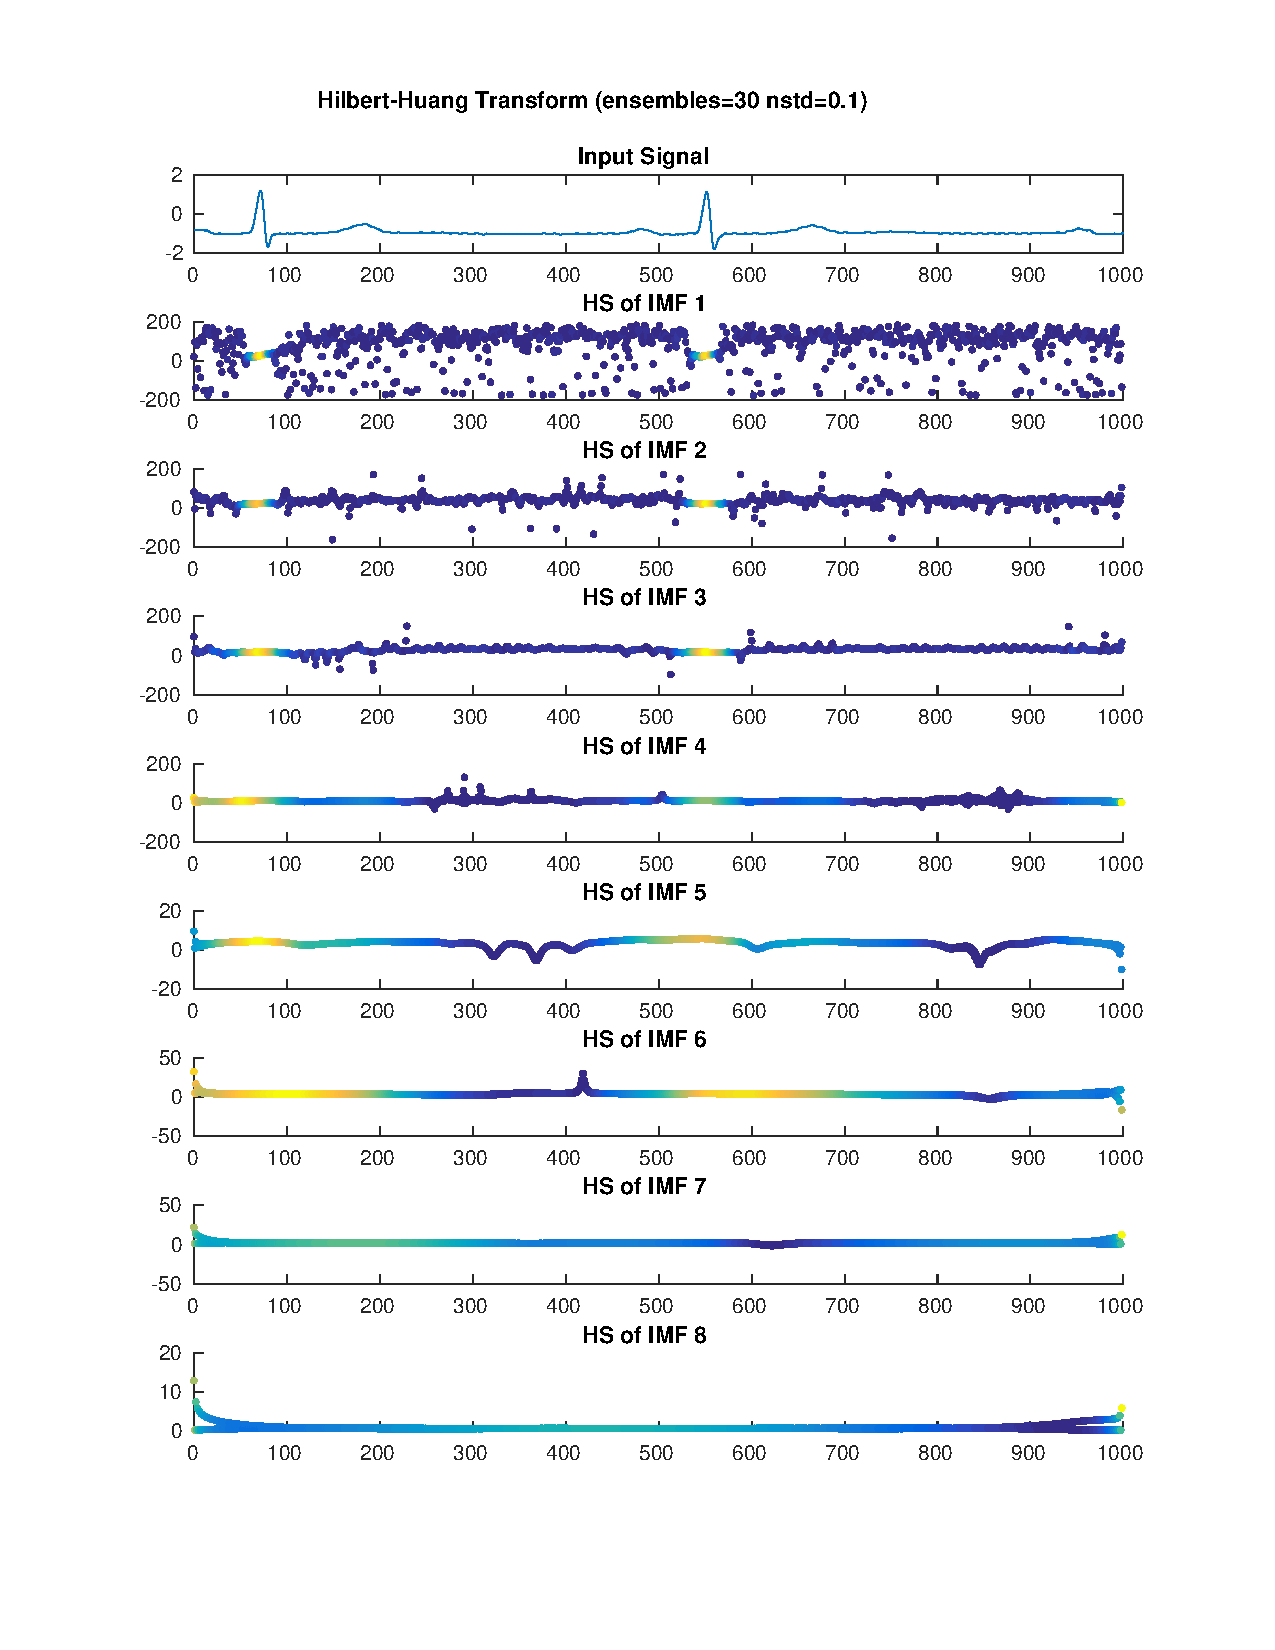
\includegraphics[width=\textwidth]{fig/123l1_hht_ensemble.pdf}
	
	(β)
\end{minipage}
\vfill
\caption{(α) Ensemble Emperical Mode Decomposition (β) Hilbert-Huang Transform του σήματος με $n_{ens}=50$ και $\sigma_n = 0.1$.}
\label{fig:123l1_hht_ensemble}
\end{figure}

\subsection*{118}

% --- STFT, WDF, CWT ---
\begin{figure}[H]
\centering
\begin{minipage}{0.48\textwidth}
	\centering
	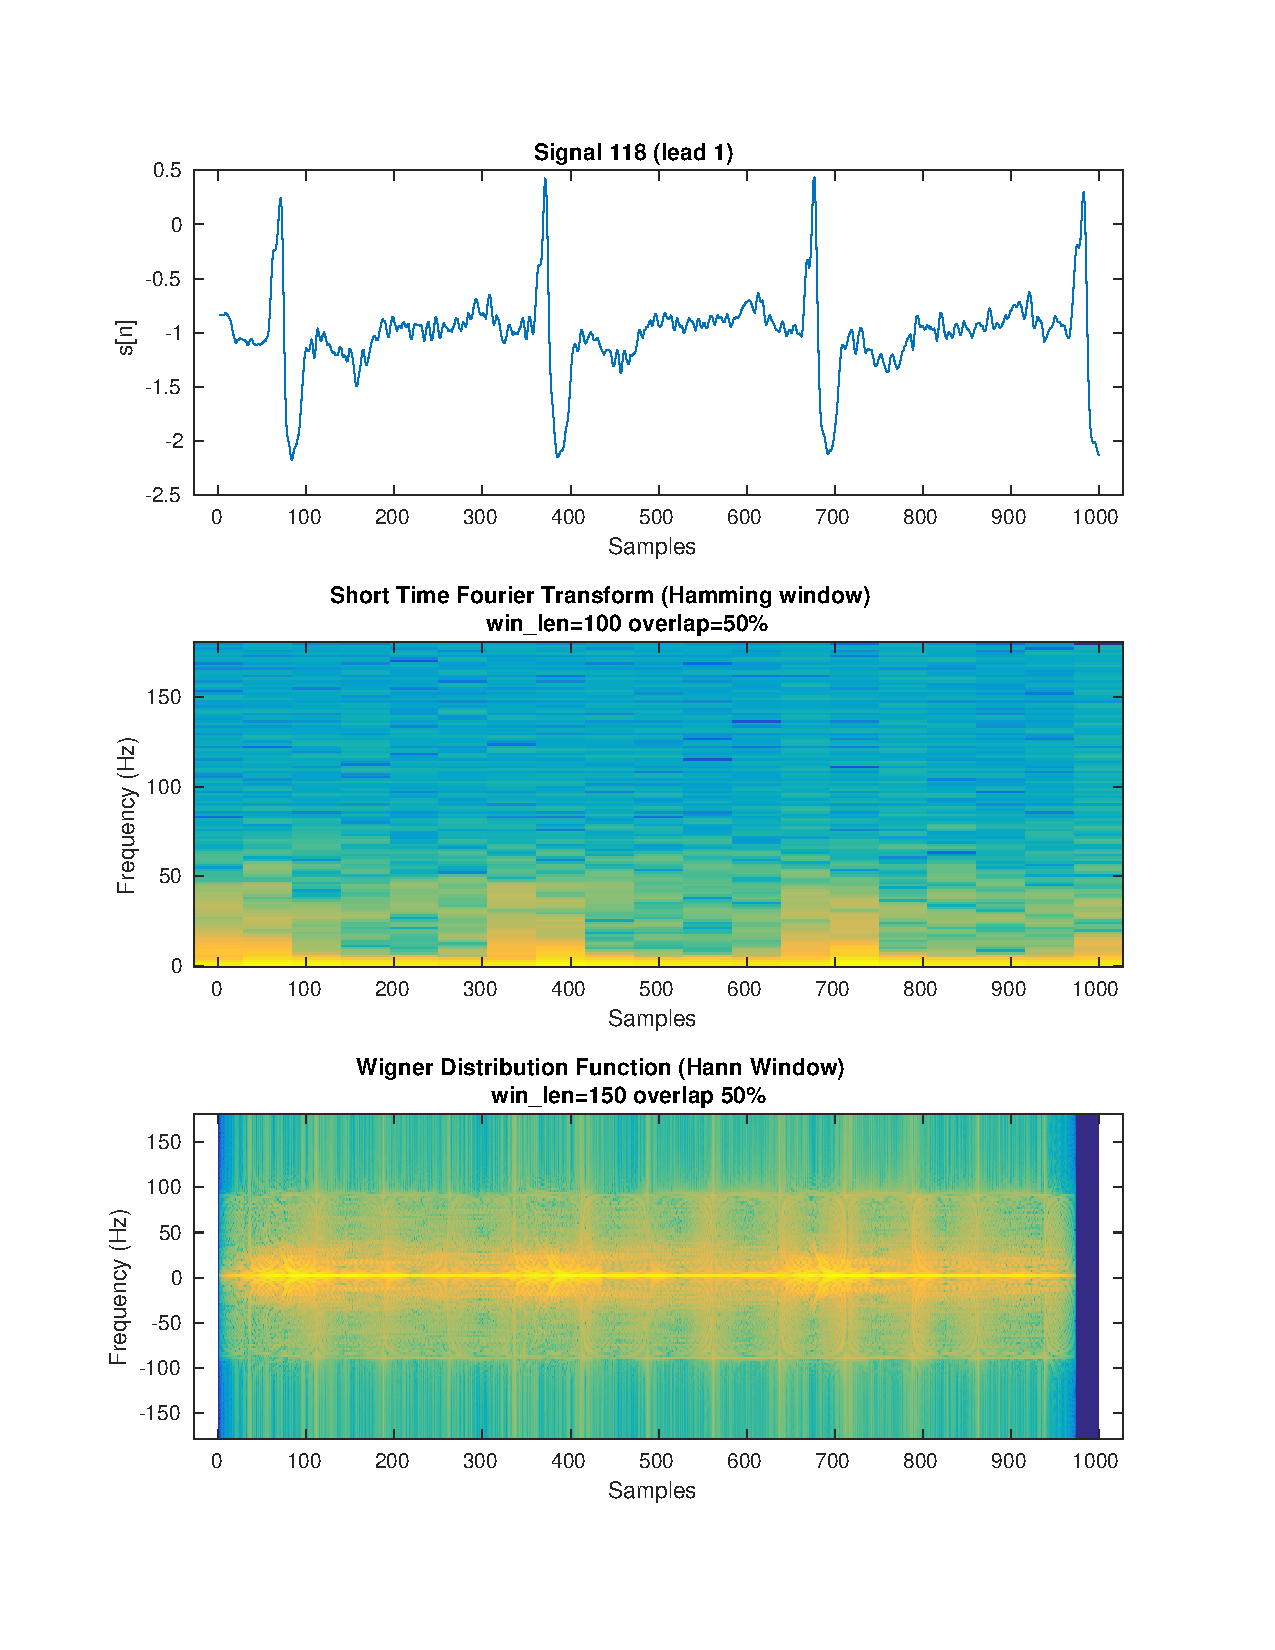
\includegraphics[width=\textwidth]{fig/118l1_stft_wdf.pdf}
	
	(α)
\end{minipage}
\begin{minipage}{0.48\textwidth}
	\centering
	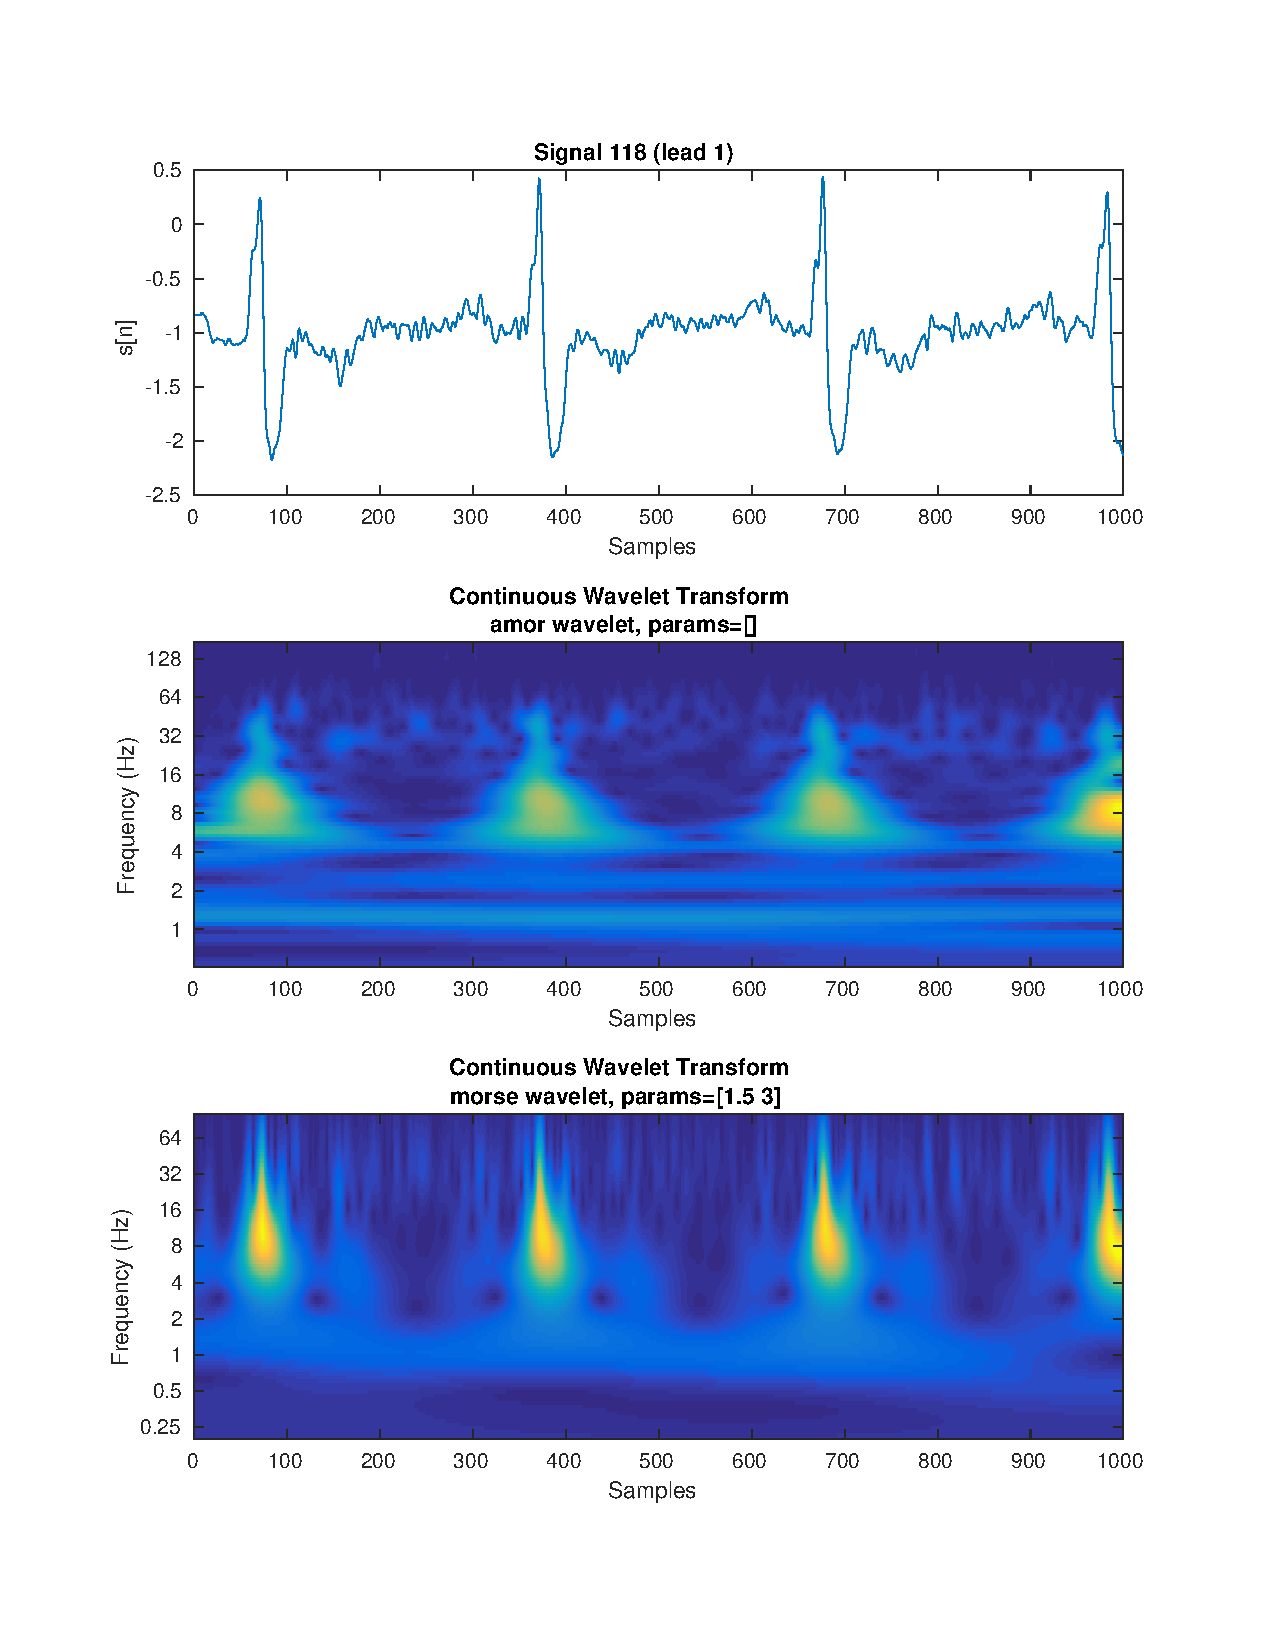
\includegraphics[width=\textwidth]{fig/118l1_cwt.pdf}
	
	(β)
\end{minipage}
\vfill
\caption{(α) Short Time Fourier Transform και Wigner Distribution Function (β) Wavelet Transform (Morlet, Morse wavelets) του σήματος.}
\label{fig:118l1_stft_wdf_wt}
\end{figure}


% --- DWT ---
\begin{figure}[H]
\centering
\begin{minipage}{0.48\textwidth}
	\centering
	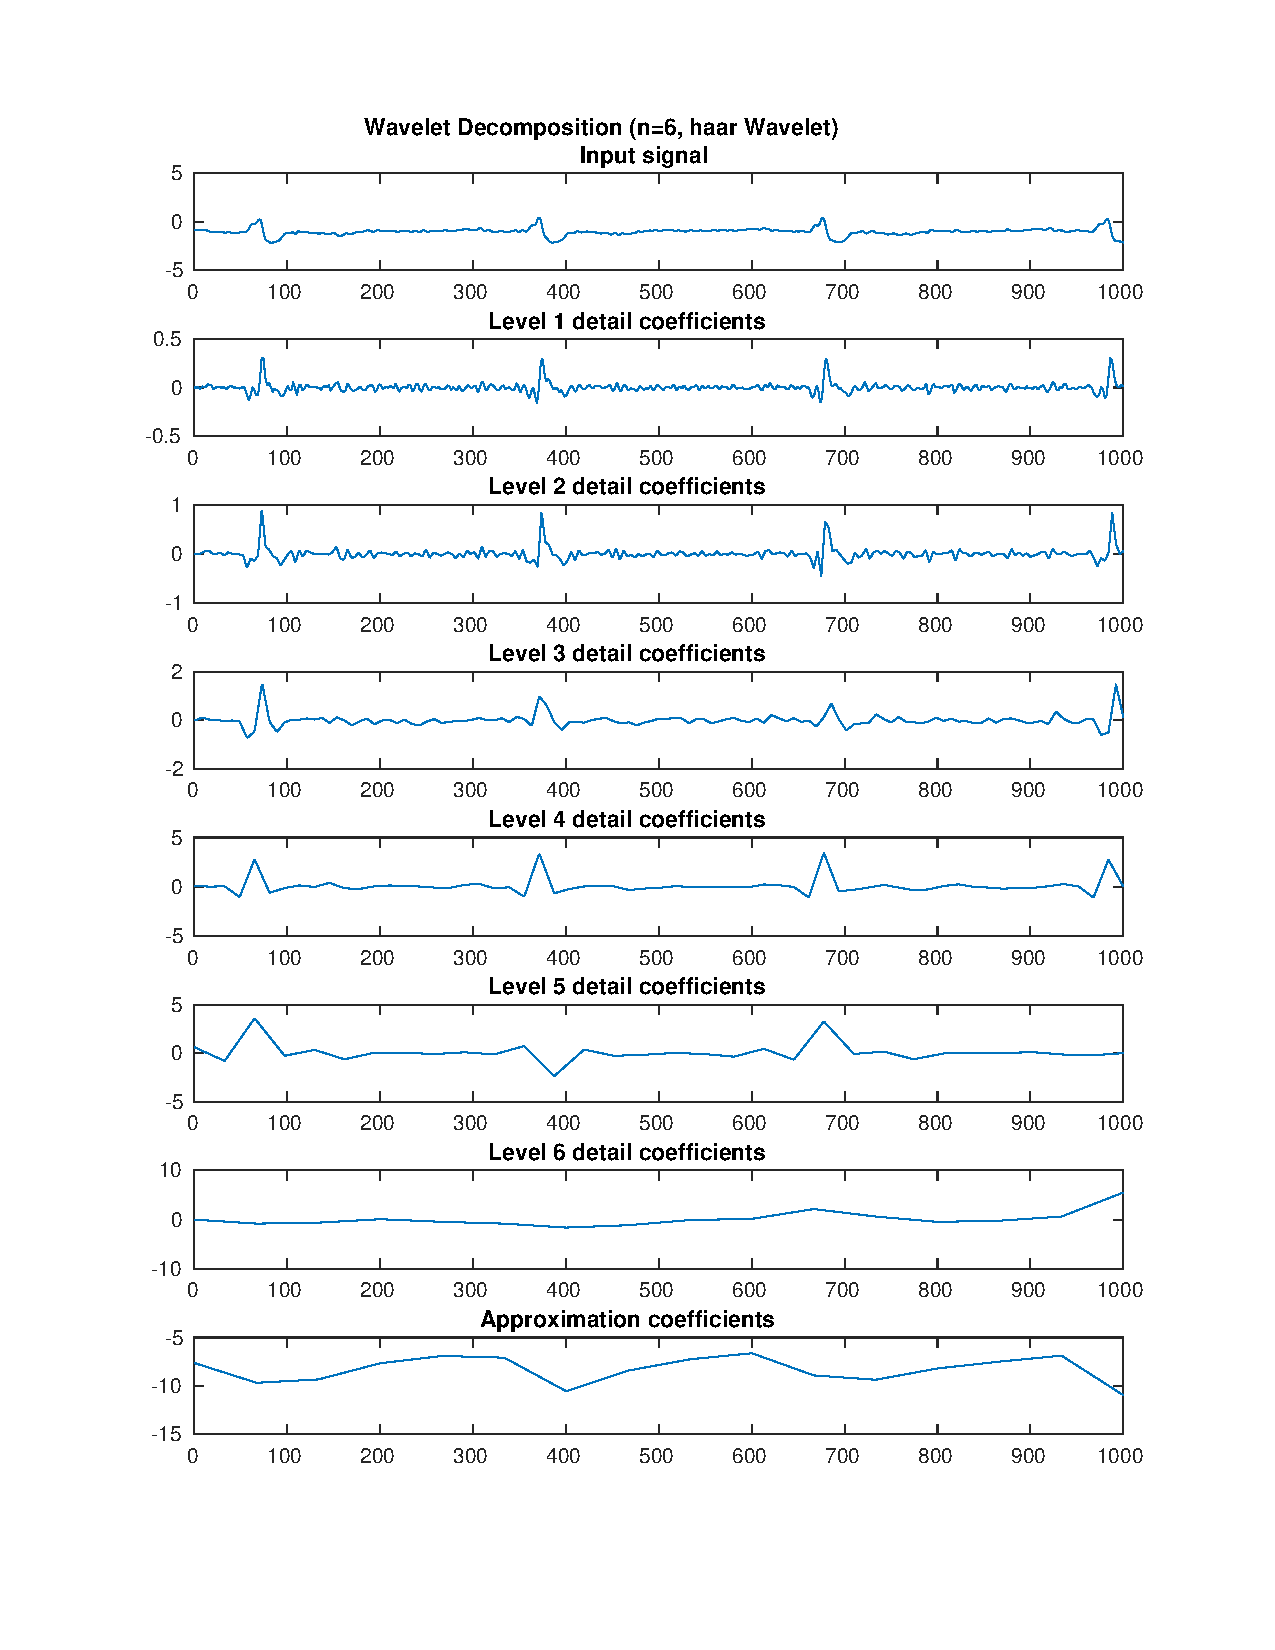
\includegraphics[width=\textwidth]{fig/118l1_dwt1.pdf}
	
	(α)
\end{minipage}
\begin{minipage}{0.48\textwidth}
	\centering
	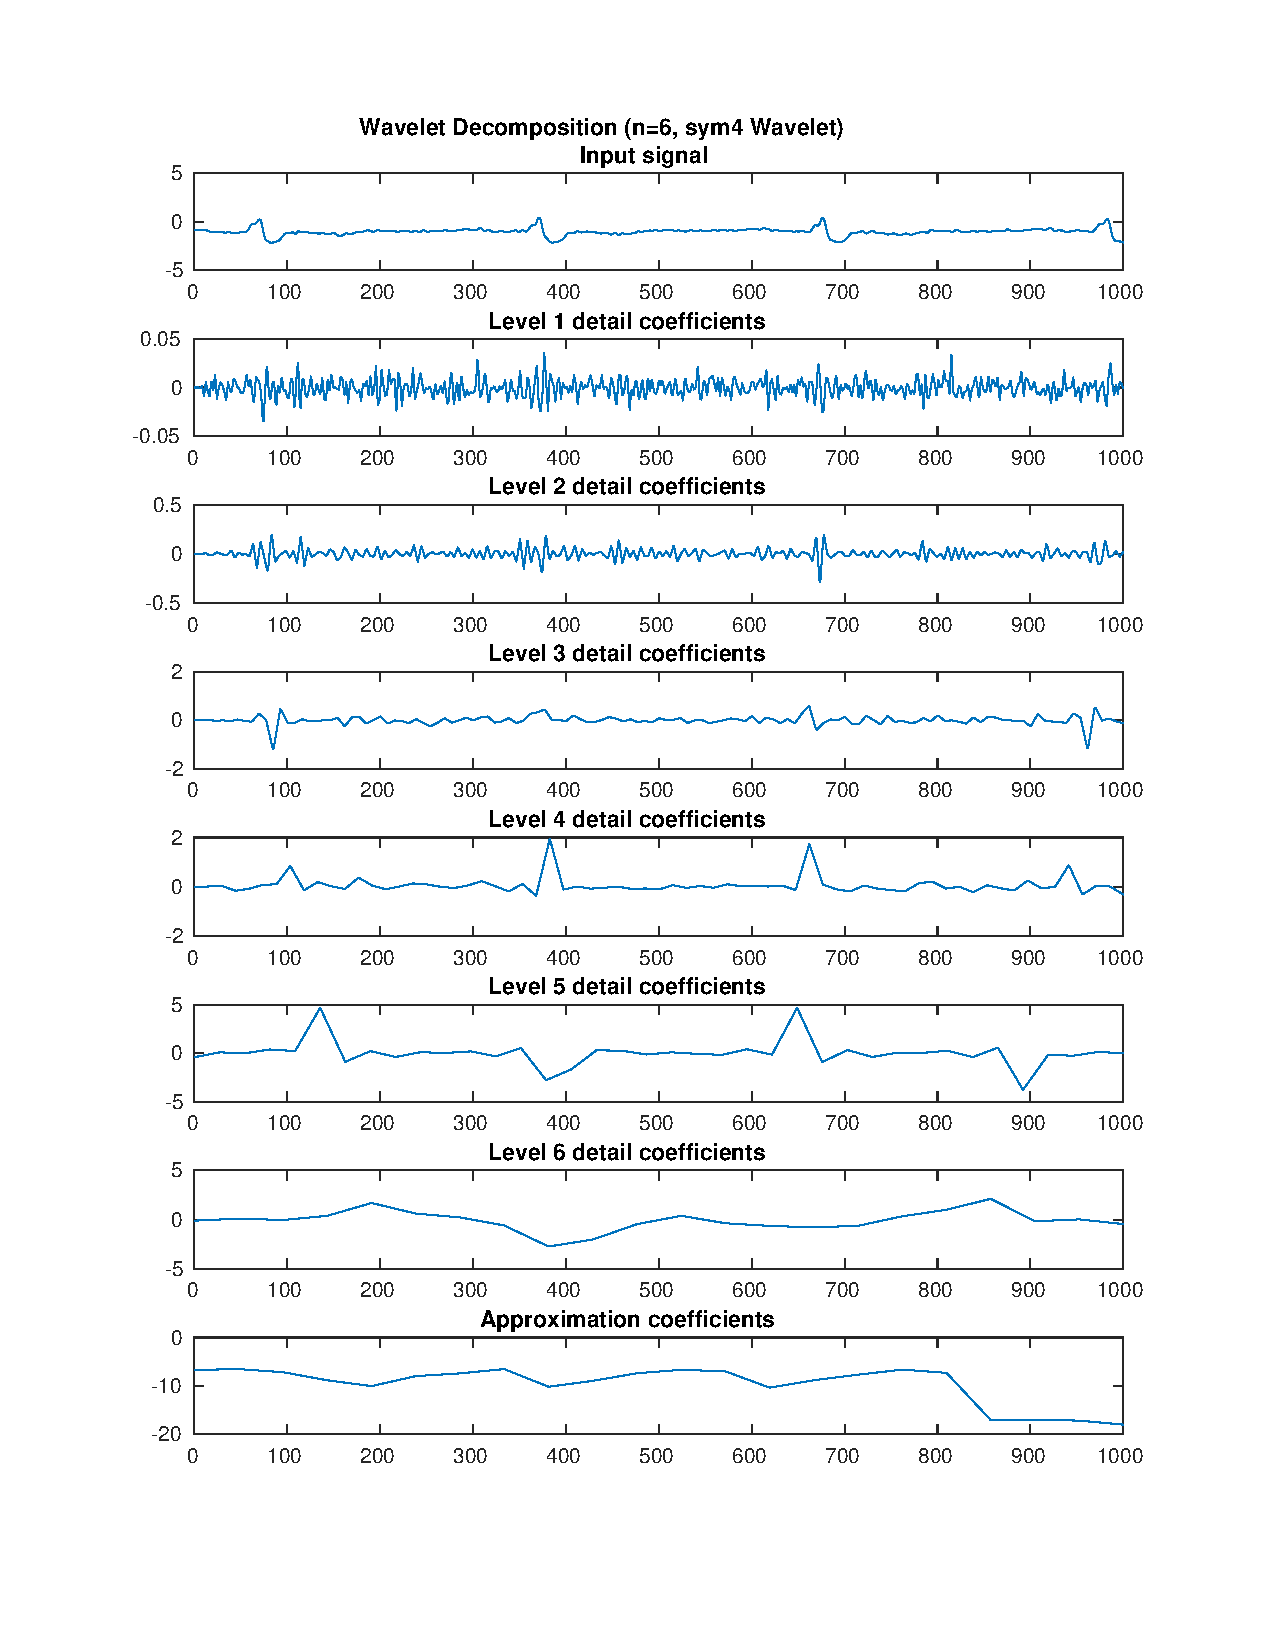
\includegraphics[width=\textwidth]{fig/118l1_dwt2.pdf}
	
	(β)
\end{minipage}
\vfill
\caption{Wavelet Decomposition του σήματος χρησιμοποιώντας wavelet (α) Haar (β) Symlet4.}
\label{fig:118l1_dwt}
\end{figure}


% --- EMD/HHT ---
\begin{figure}[H]
\centering
\begin{minipage}{0.48\textwidth}
	\centering
	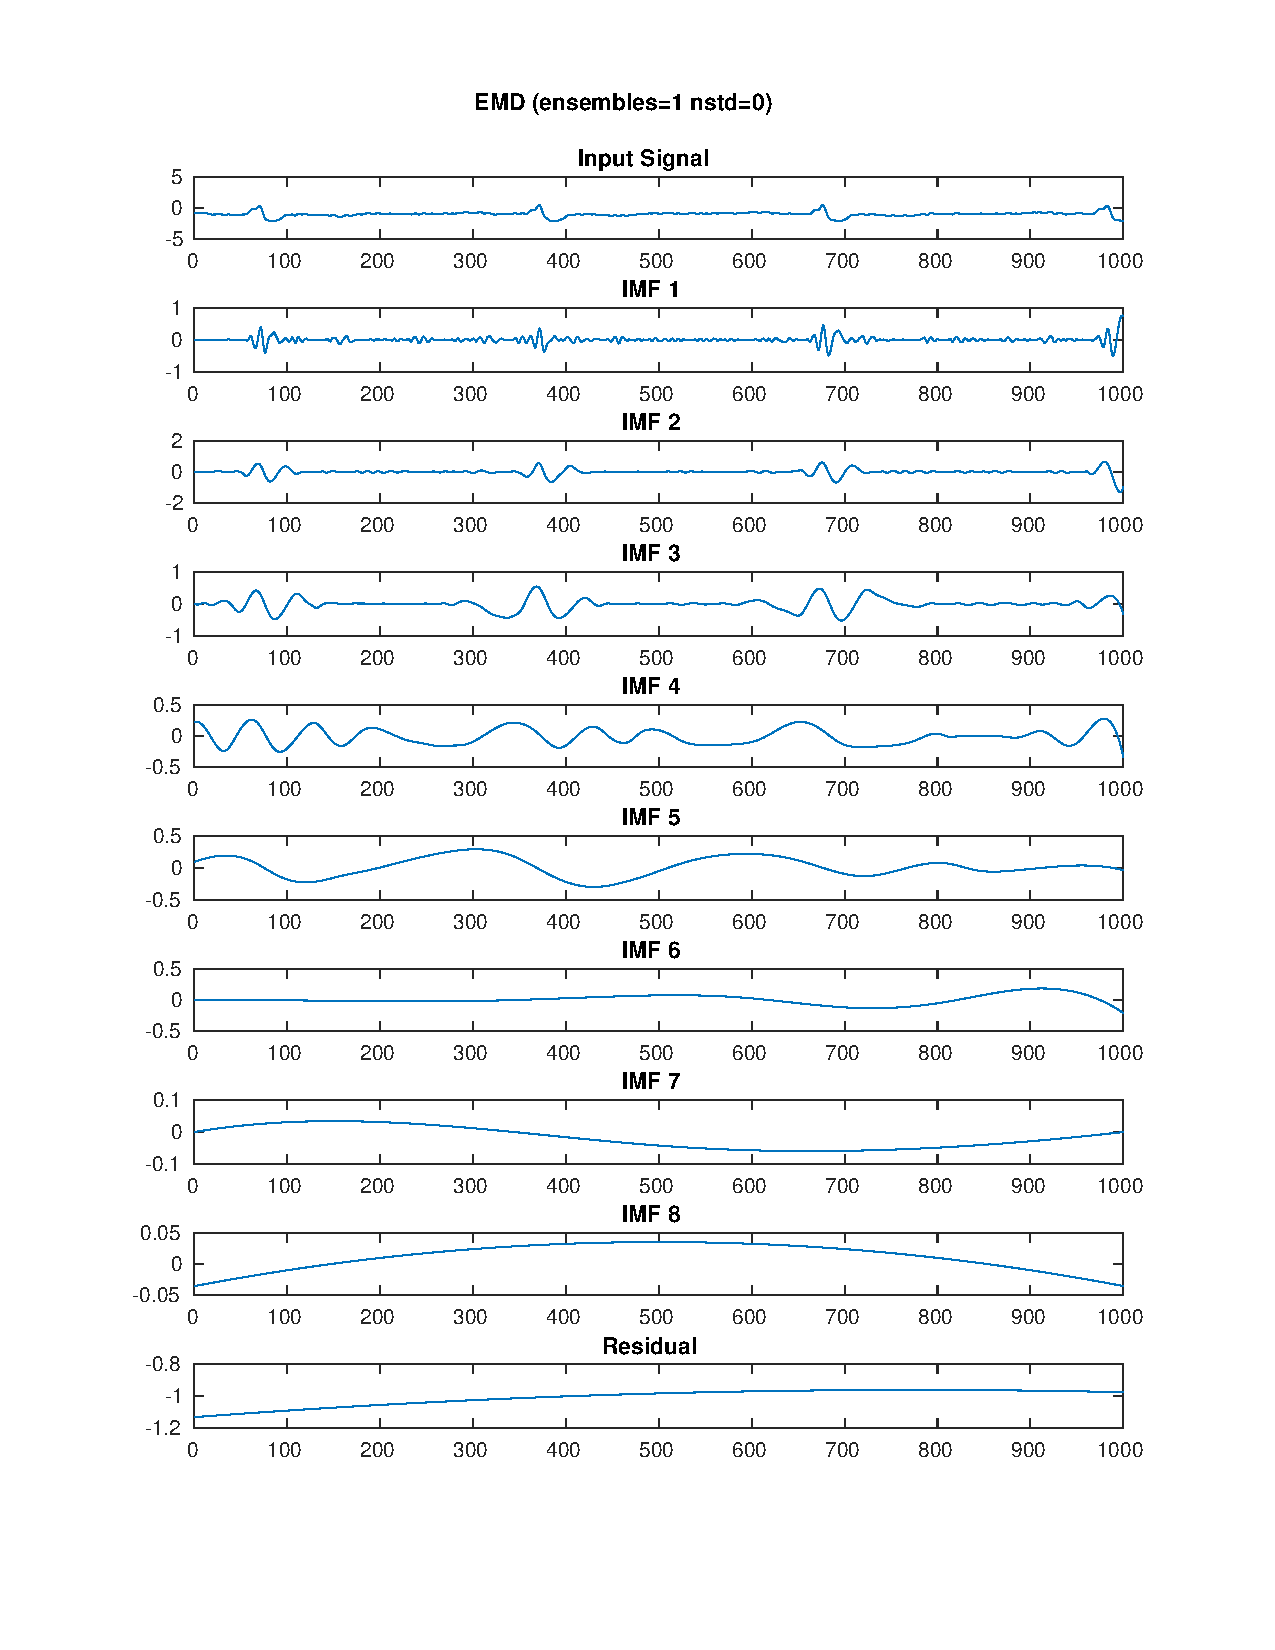
\includegraphics[width=\textwidth]{fig/118l1_emd.pdf}
	
	(α)
\end{minipage}
\begin{minipage}{0.48\textwidth}
	\centering
	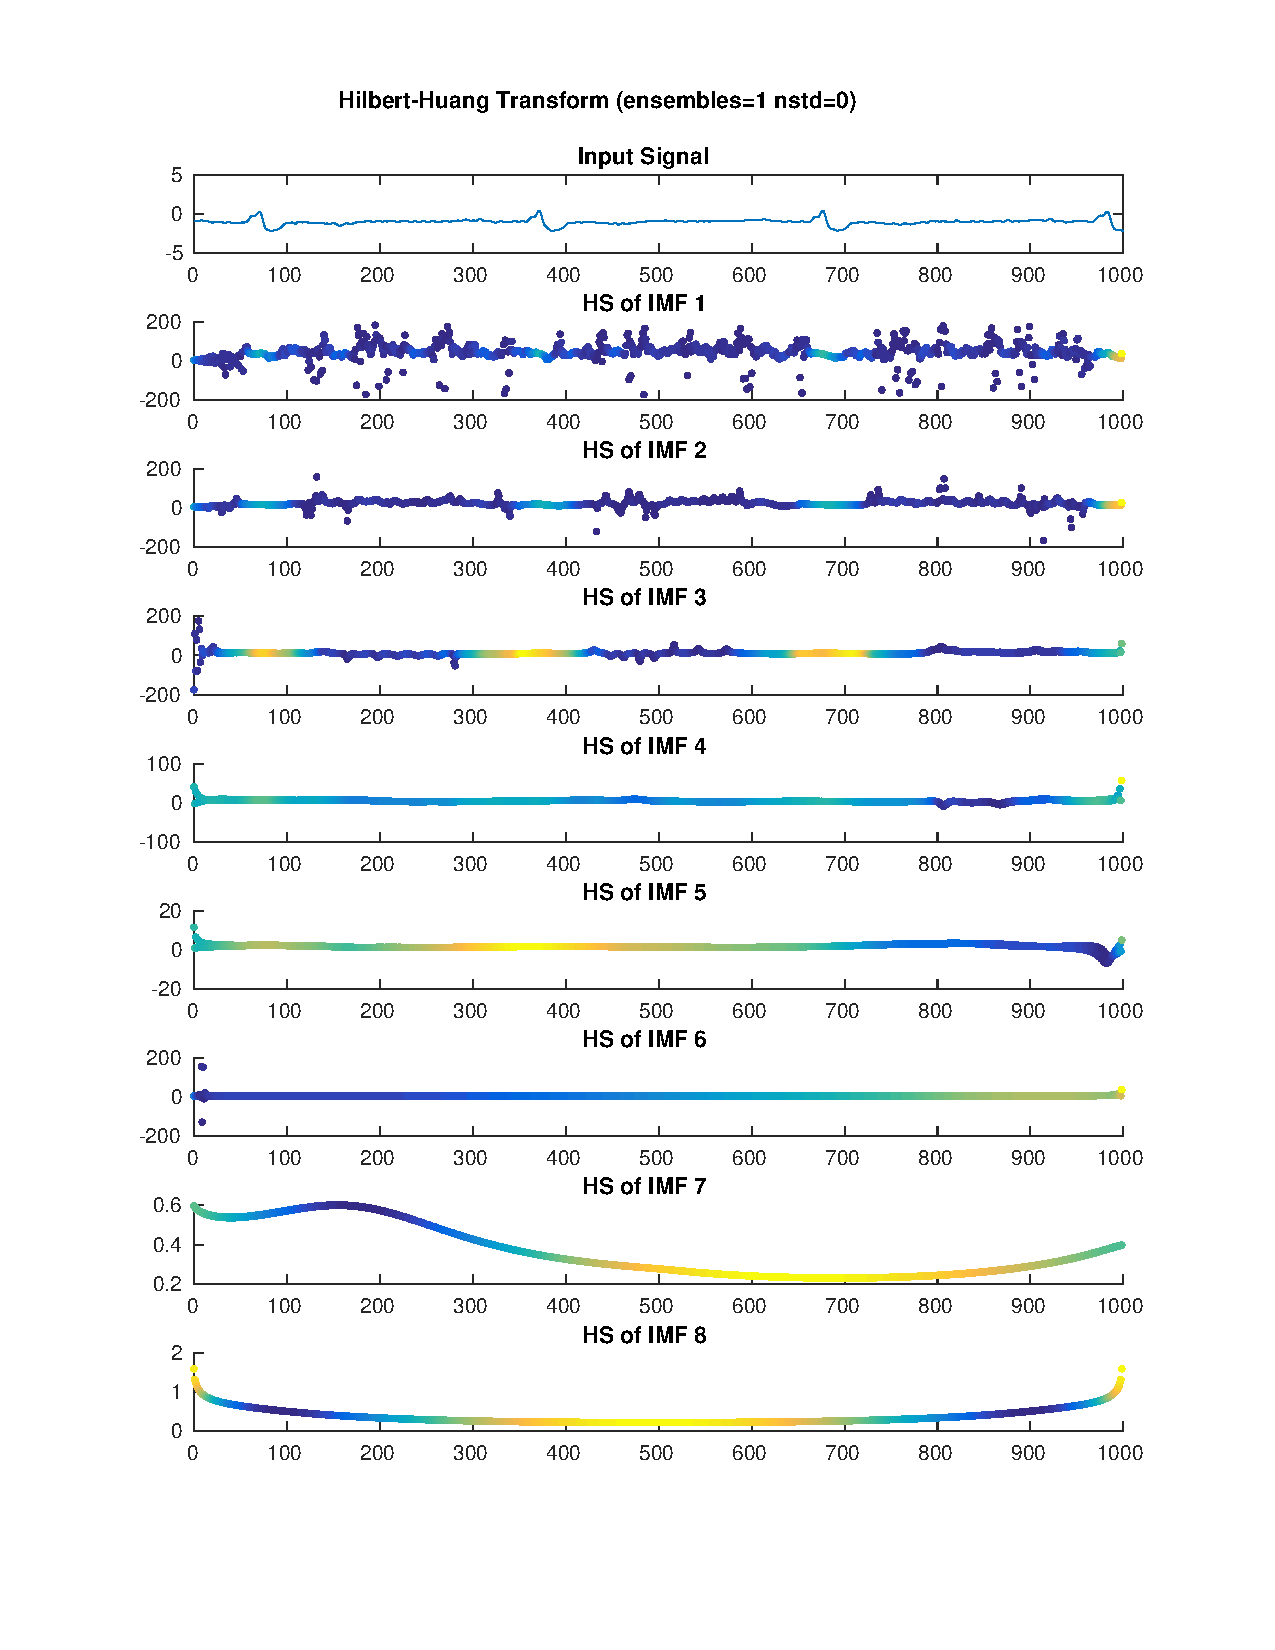
\includegraphics[width=\textwidth]{fig/118l1_hht.pdf}
	
	(β)
\end{minipage}
\vfill
\caption{(α) Emperical Mode Decomposition (β) Hilbert-Huang Transform του σήματος.}
\label{fig:118l1_hht}
\end{figure}


% --- EEMD/HHT ---
\begin{figure}[H]
\centering
\begin{minipage}{0.48\textwidth}
	\centering
	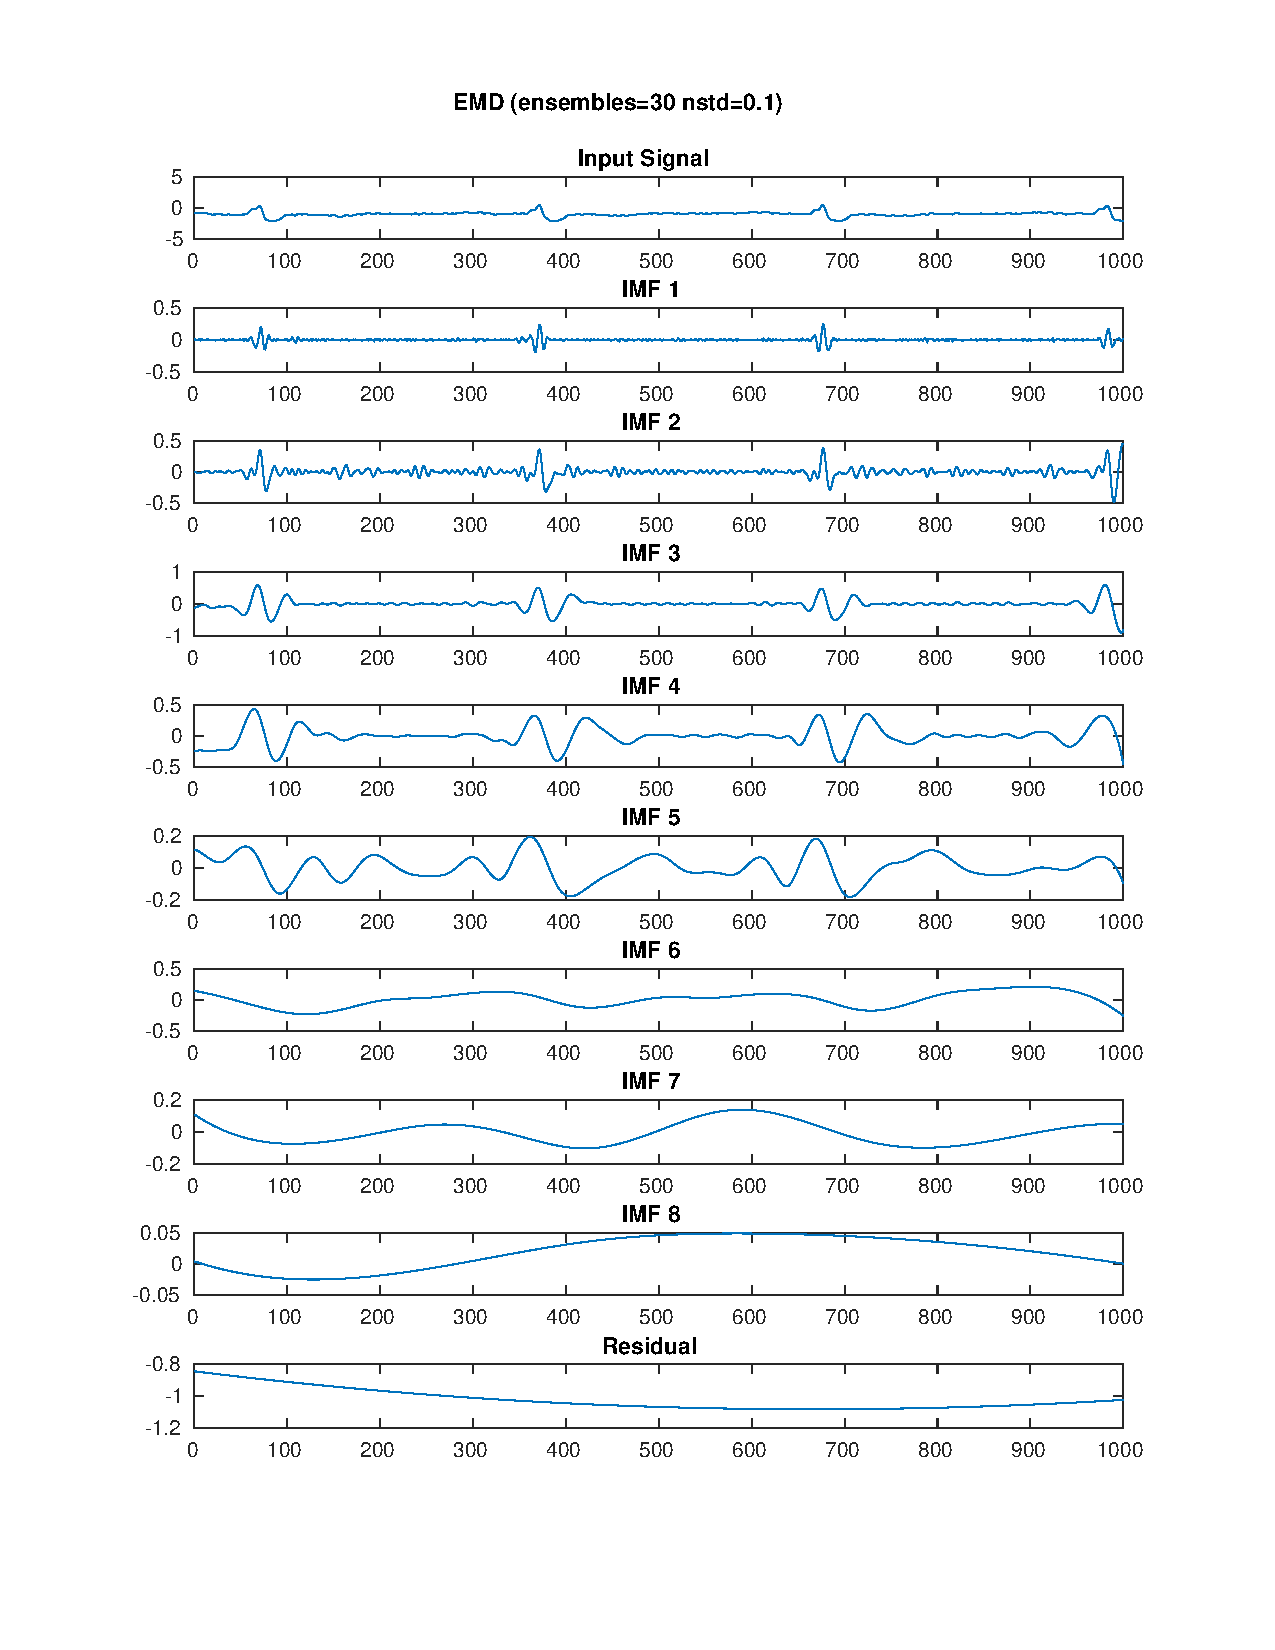
\includegraphics[width=\textwidth]{fig/118l1_emd_ensemble.pdf}
	
	(α)
\end{minipage}
\begin{minipage}{0.48\textwidth}
	\centering
	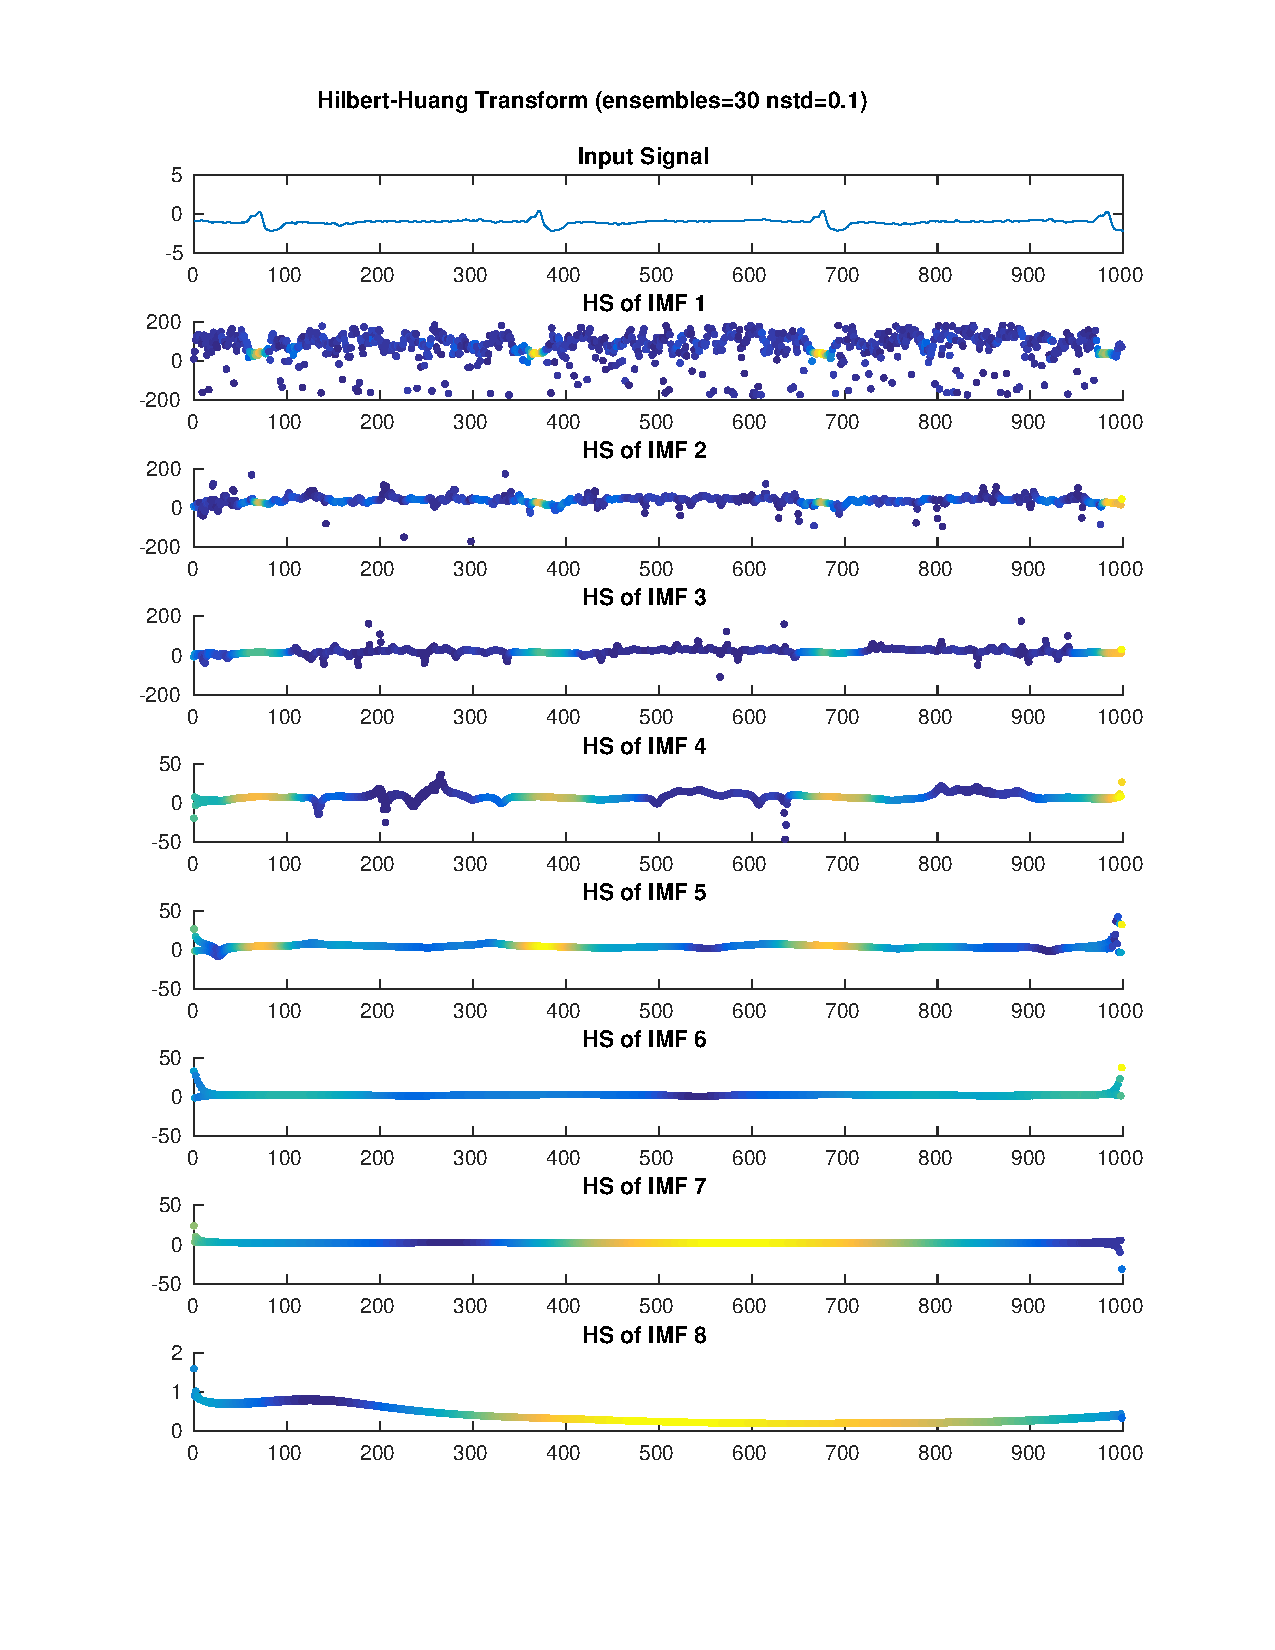
\includegraphics[width=\textwidth]{fig/118l1_hht_ensemble.pdf}
	
	(β)
\end{minipage}
\vfill
\caption{(α) Ensemble Emperical Mode Decomposition (β) Hilbert-Huang Transform του σήματος με $n_{ens}=50$ και $\sigma_n = 0.1$.}
\label{fig:118l1_hht_ensemble}
\end{figure}

\subsection*{217}

% --- STFT, WDF, CWT ---
\begin{figure}[H]
\centering
\begin{minipage}{0.48\textwidth}
	\centering
	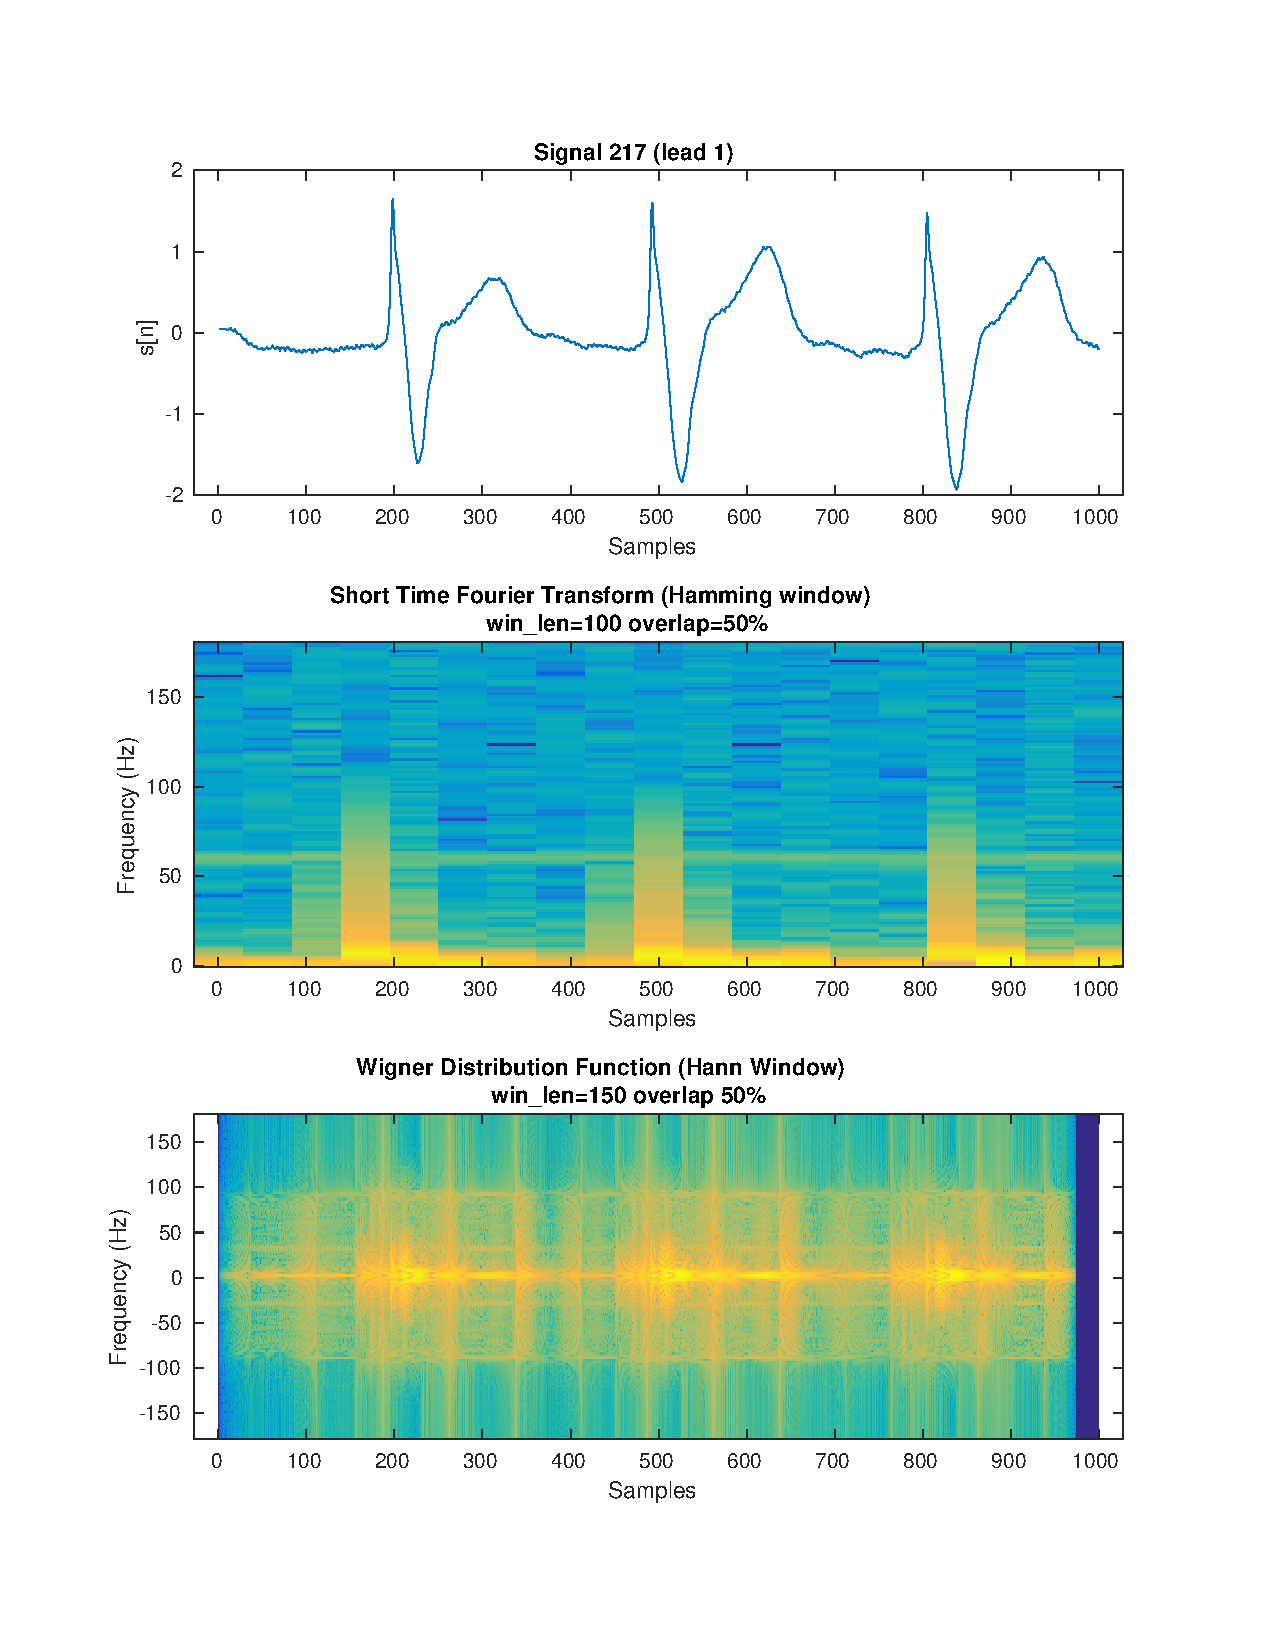
\includegraphics[width=\textwidth]{fig/217l1_stft_wdf.pdf}
	
	(α)
\end{minipage}
\begin{minipage}{0.48\textwidth}
	\centering
	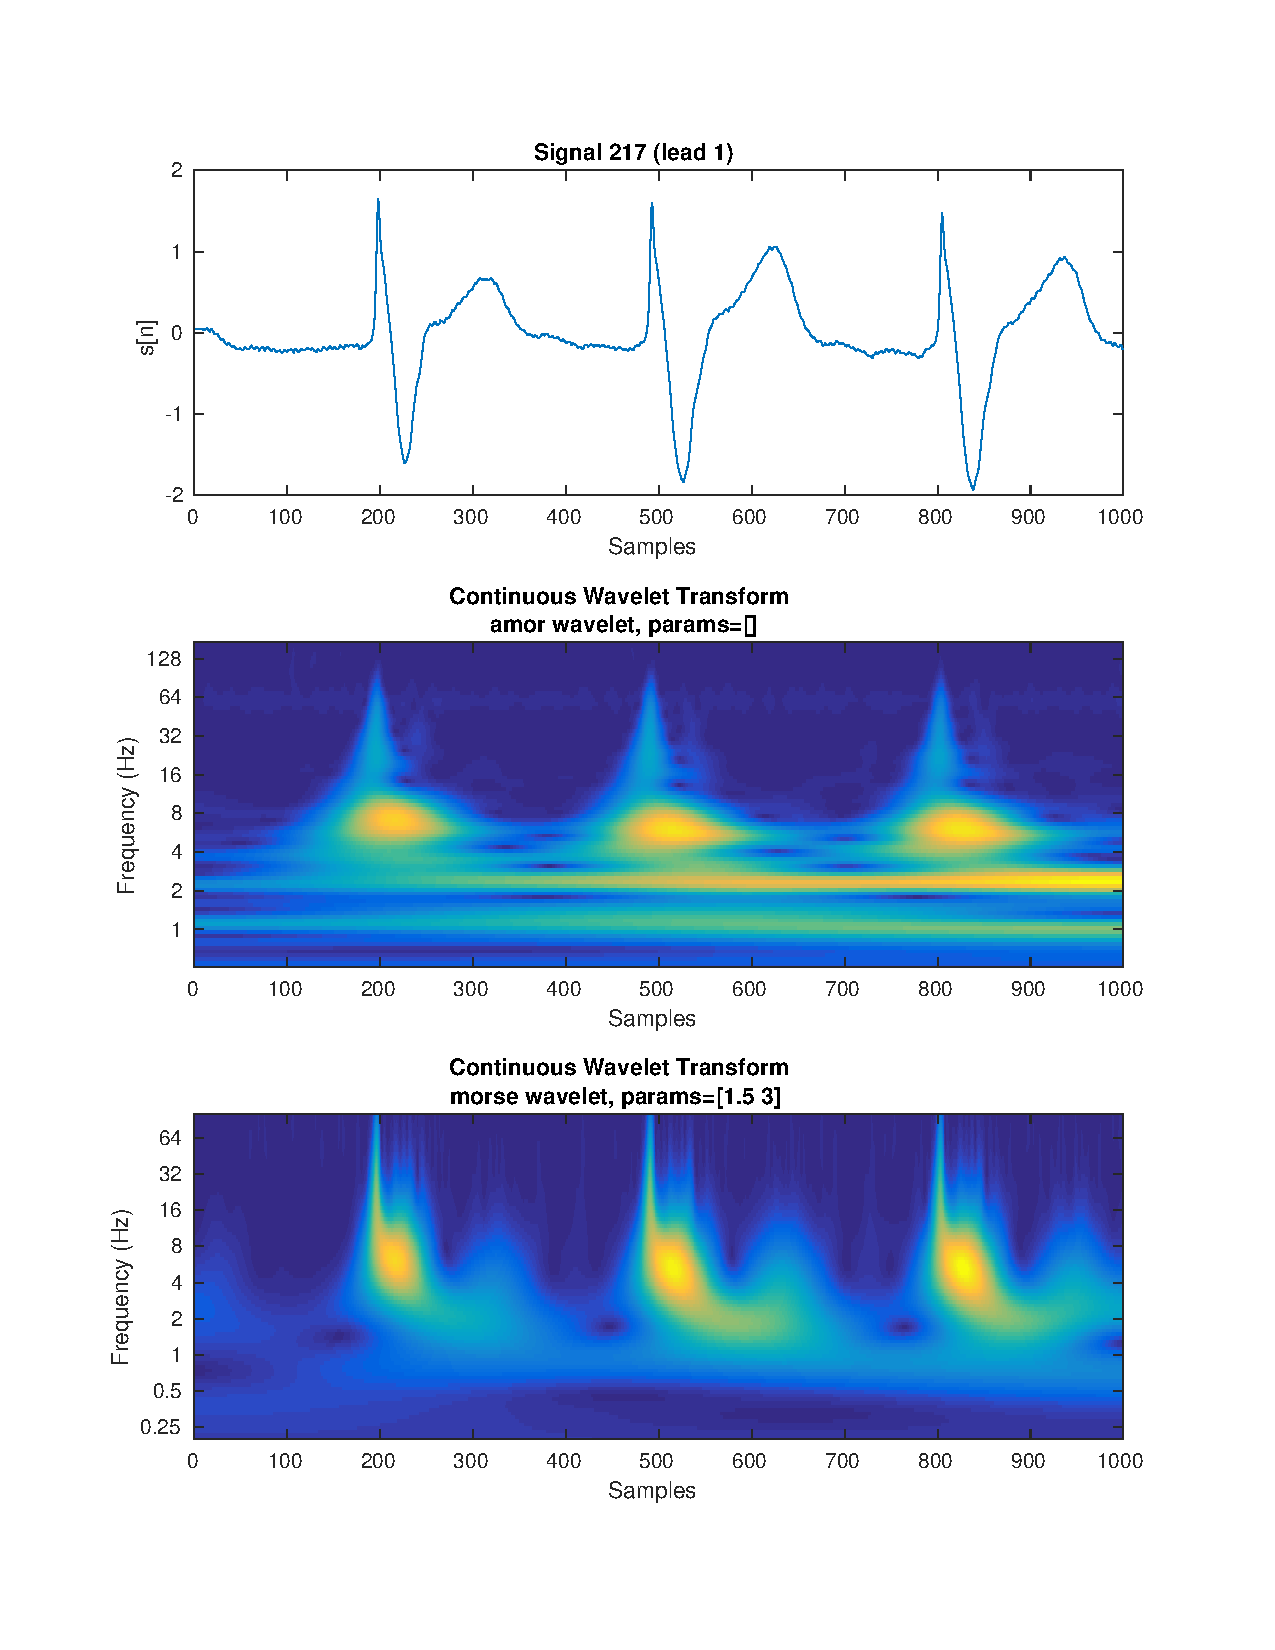
\includegraphics[width=\textwidth]{fig/217l1_cwt.pdf}
	
	(β)
\end{minipage}
\vfill
\caption{(α) Short Time Fourier Transform και Wigner Distribution Function (β) Wavelet Transform (Morlet, Morse wavelets) του σήματος.}
\label{fig:217l1_stft_wdf_wt}
\end{figure}


% --- DWT ---
\begin{figure}[H]
\centering
\begin{minipage}{0.48\textwidth}
	\centering
	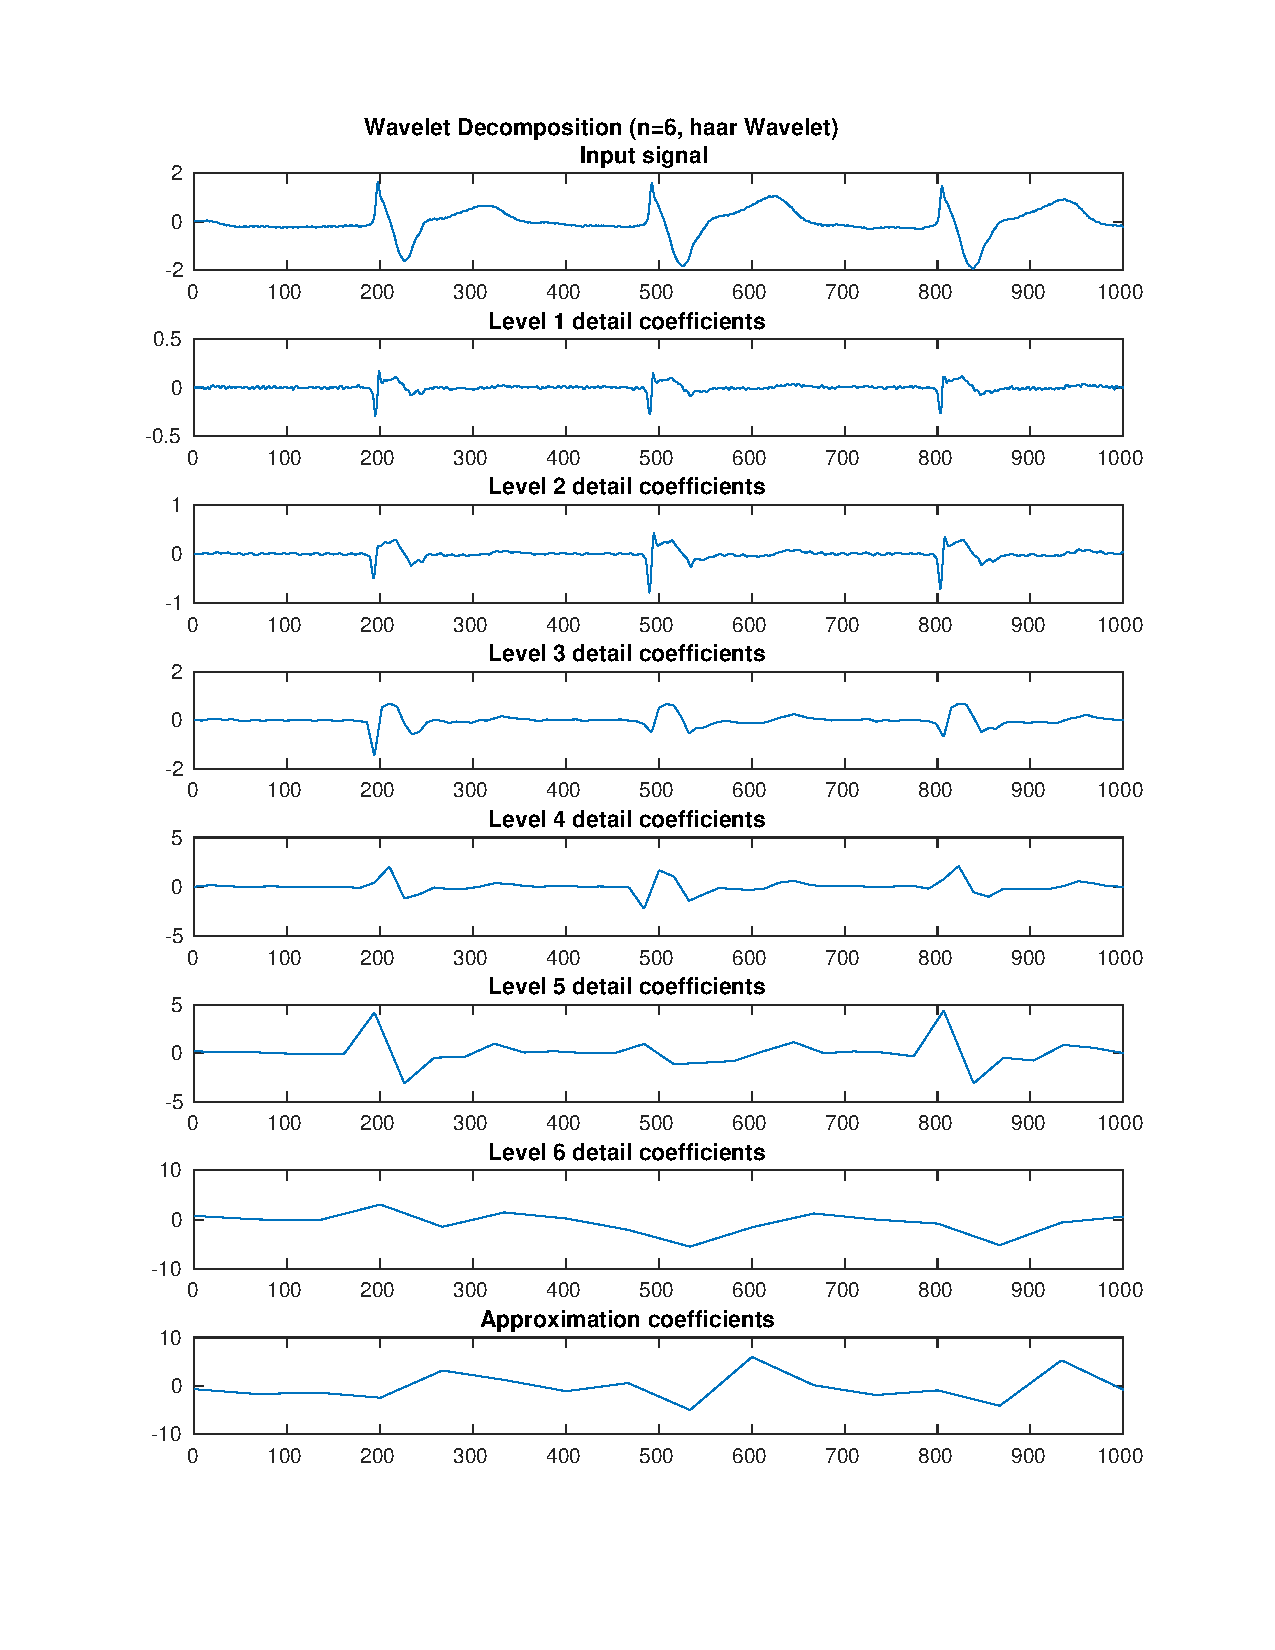
\includegraphics[width=\textwidth]{fig/217l1_dwt1.pdf}
	
	(α)
\end{minipage}
\begin{minipage}{0.48\textwidth}
	\centering
	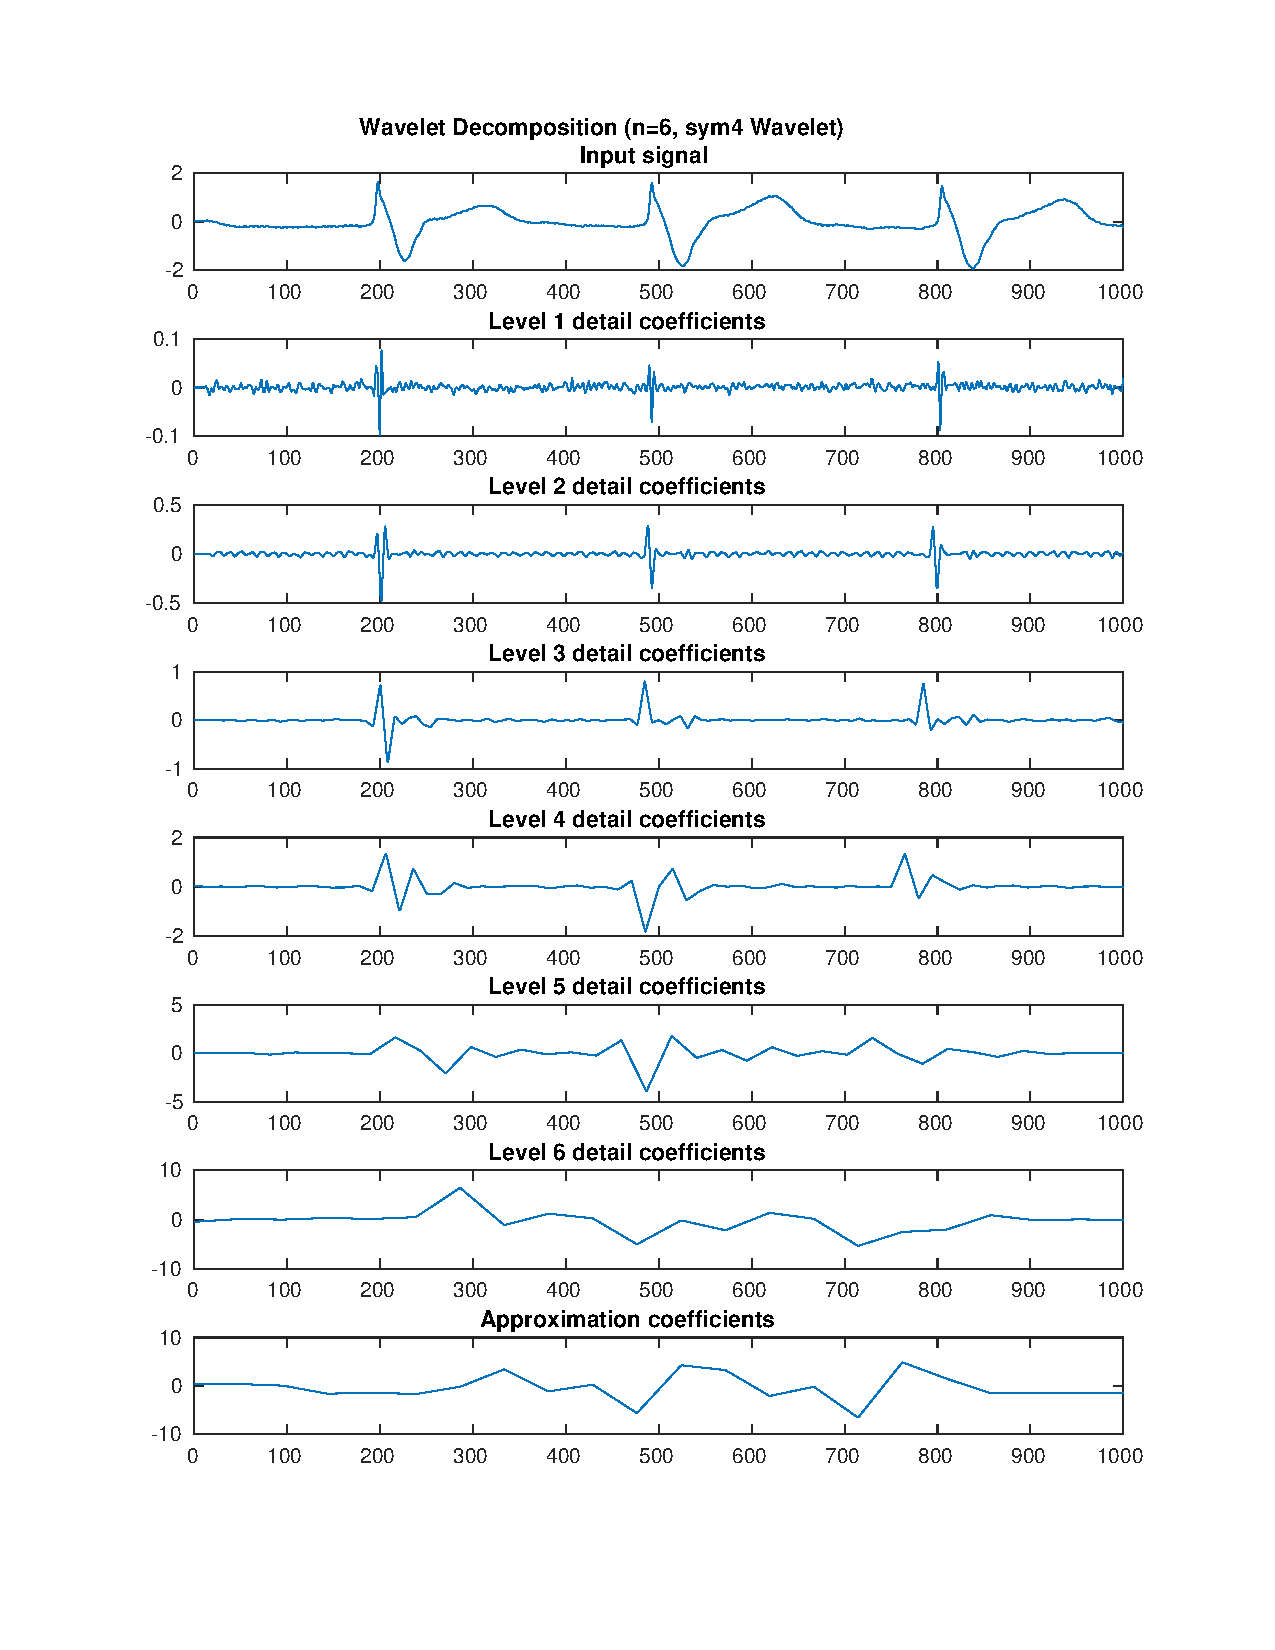
\includegraphics[width=\textwidth]{fig/217l1_dwt2.pdf}
	
	(β)
\end{minipage}
\vfill
\caption{Wavelet Decomposition του σήματος χρησιμοποιώντας wavelet (α) Haar (β) Symlet4.}
\label{fig:217l1_dwt}
\end{figure}


% --- EMD/HHT ---
\begin{figure}[H]
\centering
\begin{minipage}{0.48\textwidth}
	\centering
	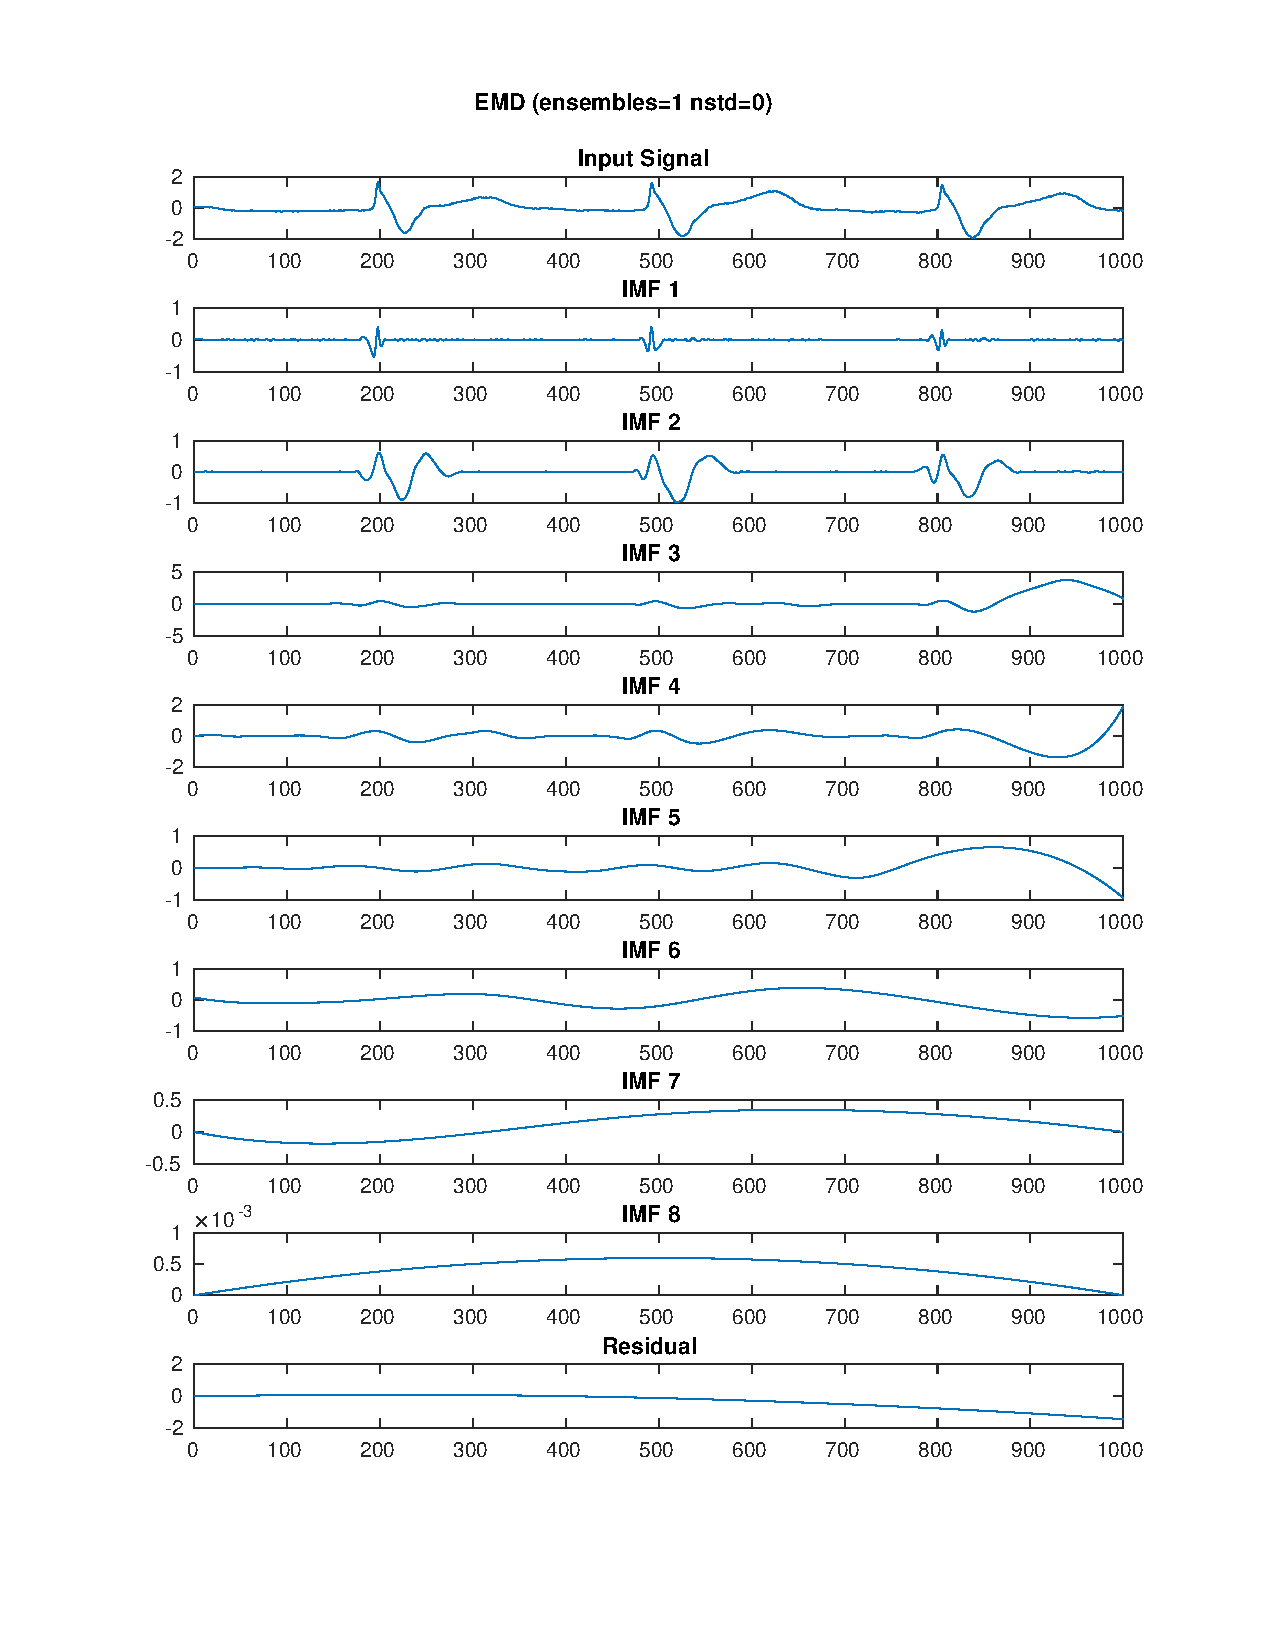
\includegraphics[width=\textwidth]{fig/217l1_emd.pdf}
	
	(α)
\end{minipage}
\begin{minipage}{0.48\textwidth}
	\centering
	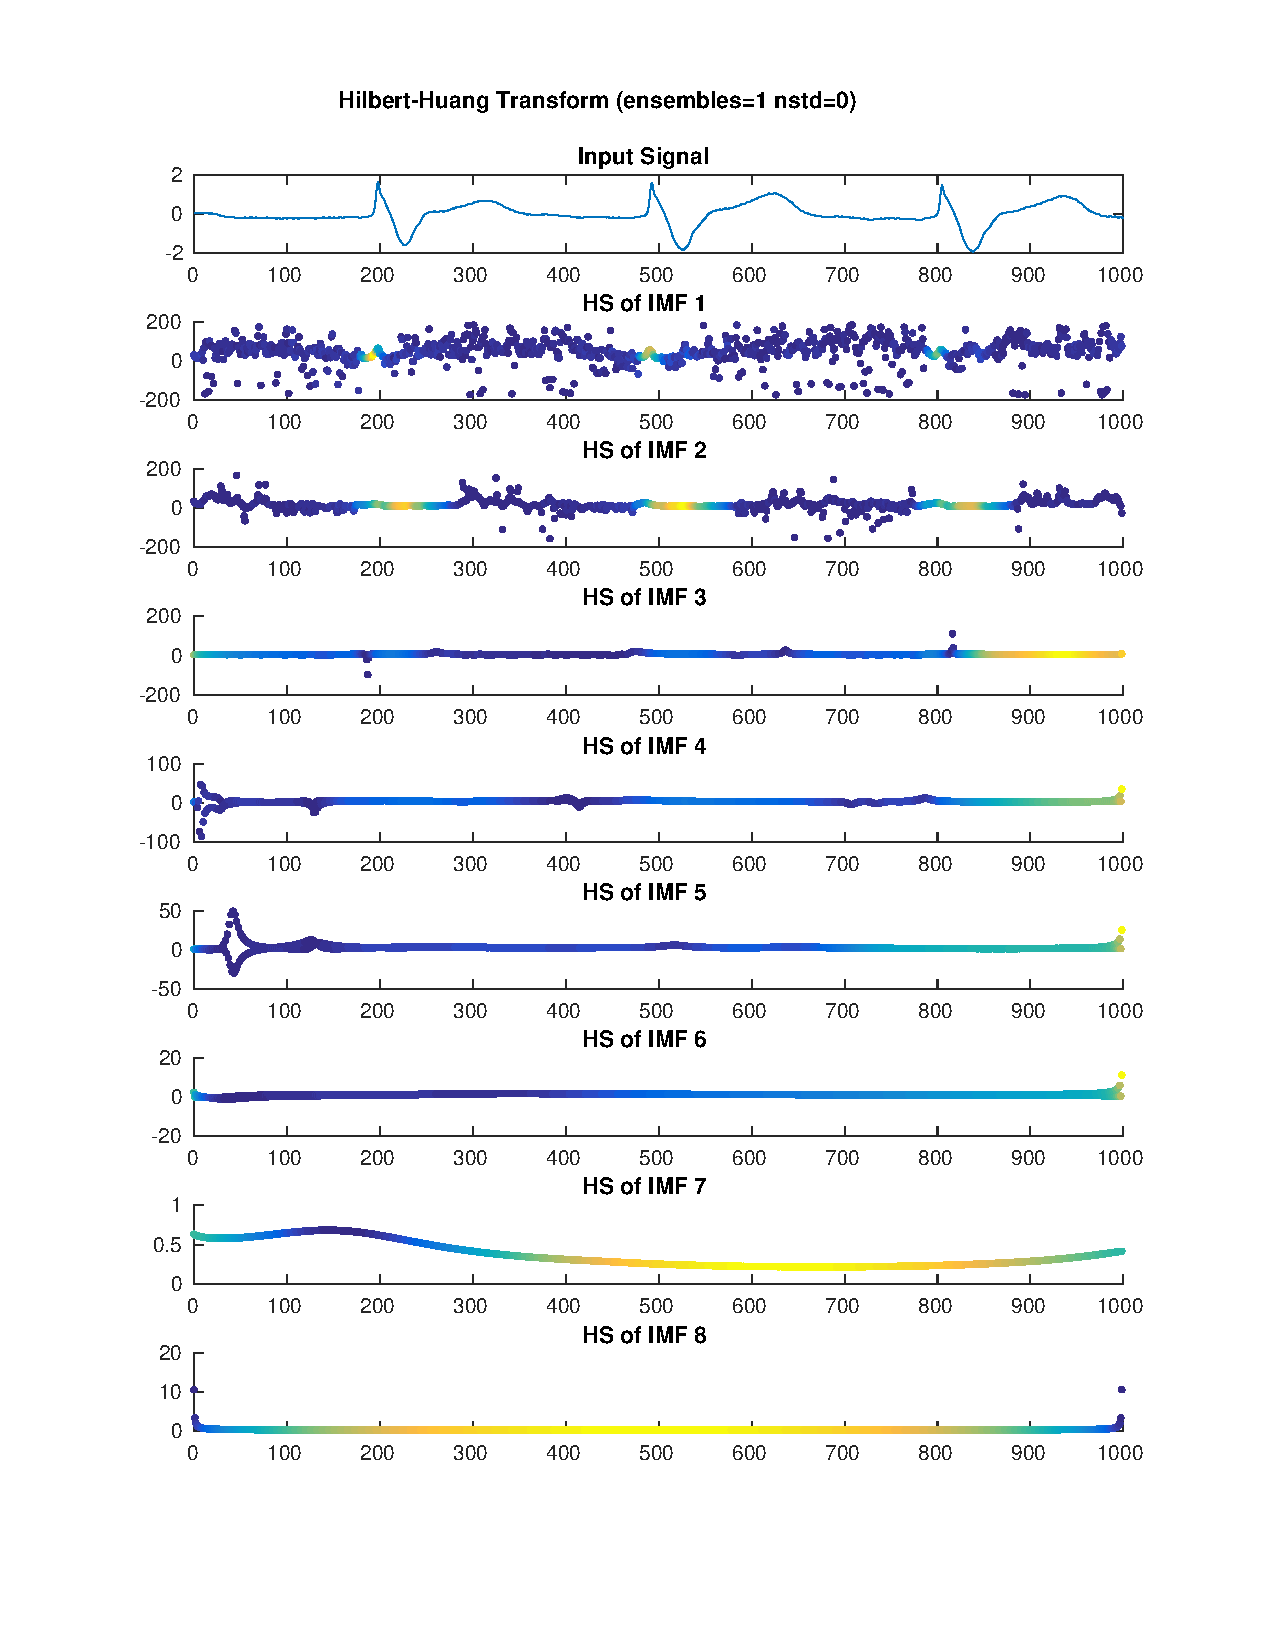
\includegraphics[width=\textwidth]{fig/217l1_hht.pdf}
	
	(β)
\end{minipage}
\vfill
\caption{(α) Emperical Mode Decomposition (β) Hilbert-Huang Transform του σήματος.}
\label{fig:217l1_hht}
\end{figure}


% --- EEMD/HHT ---
\begin{figure}[H]
\centering
\begin{minipage}{0.48\textwidth}
	\centering
	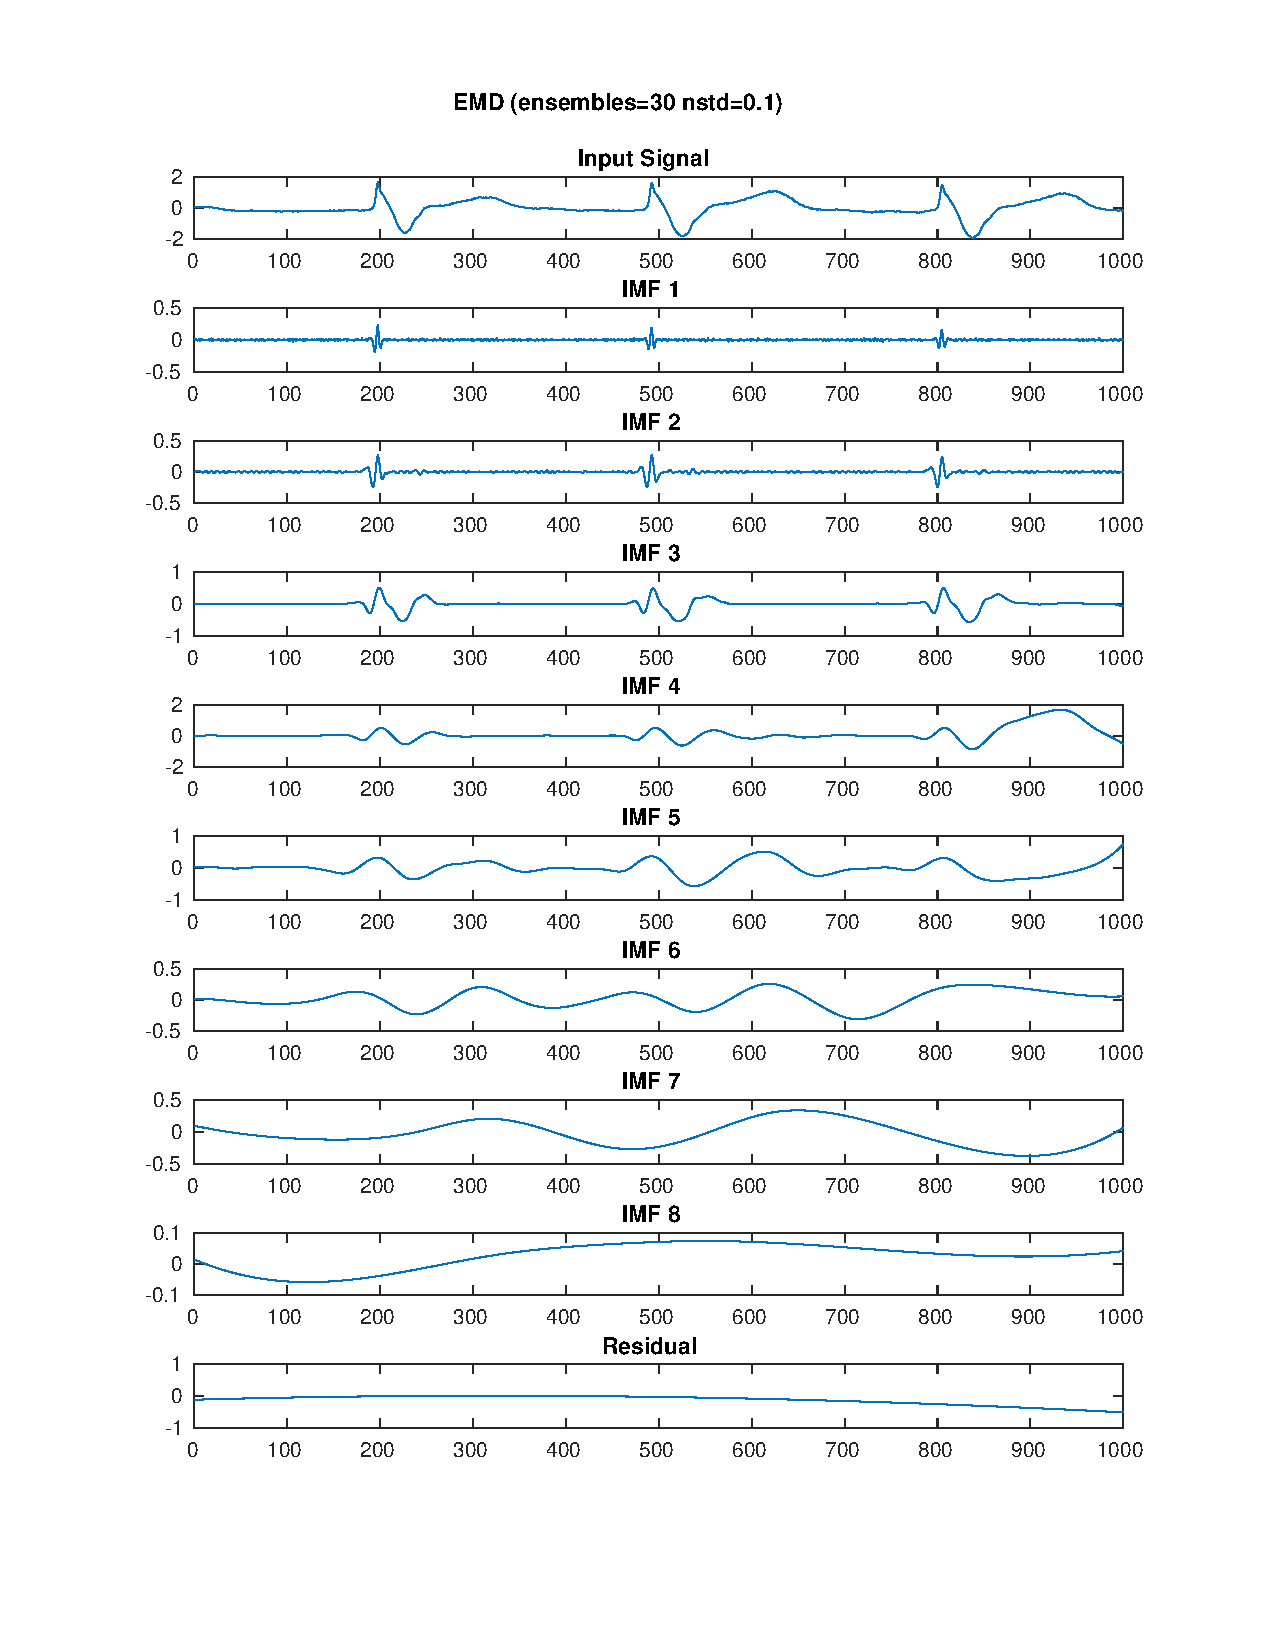
\includegraphics[width=\textwidth]{fig/217l1_emd_ensemble.pdf}
	
	(α)
\end{minipage}
\begin{minipage}{0.48\textwidth}
	\centering
	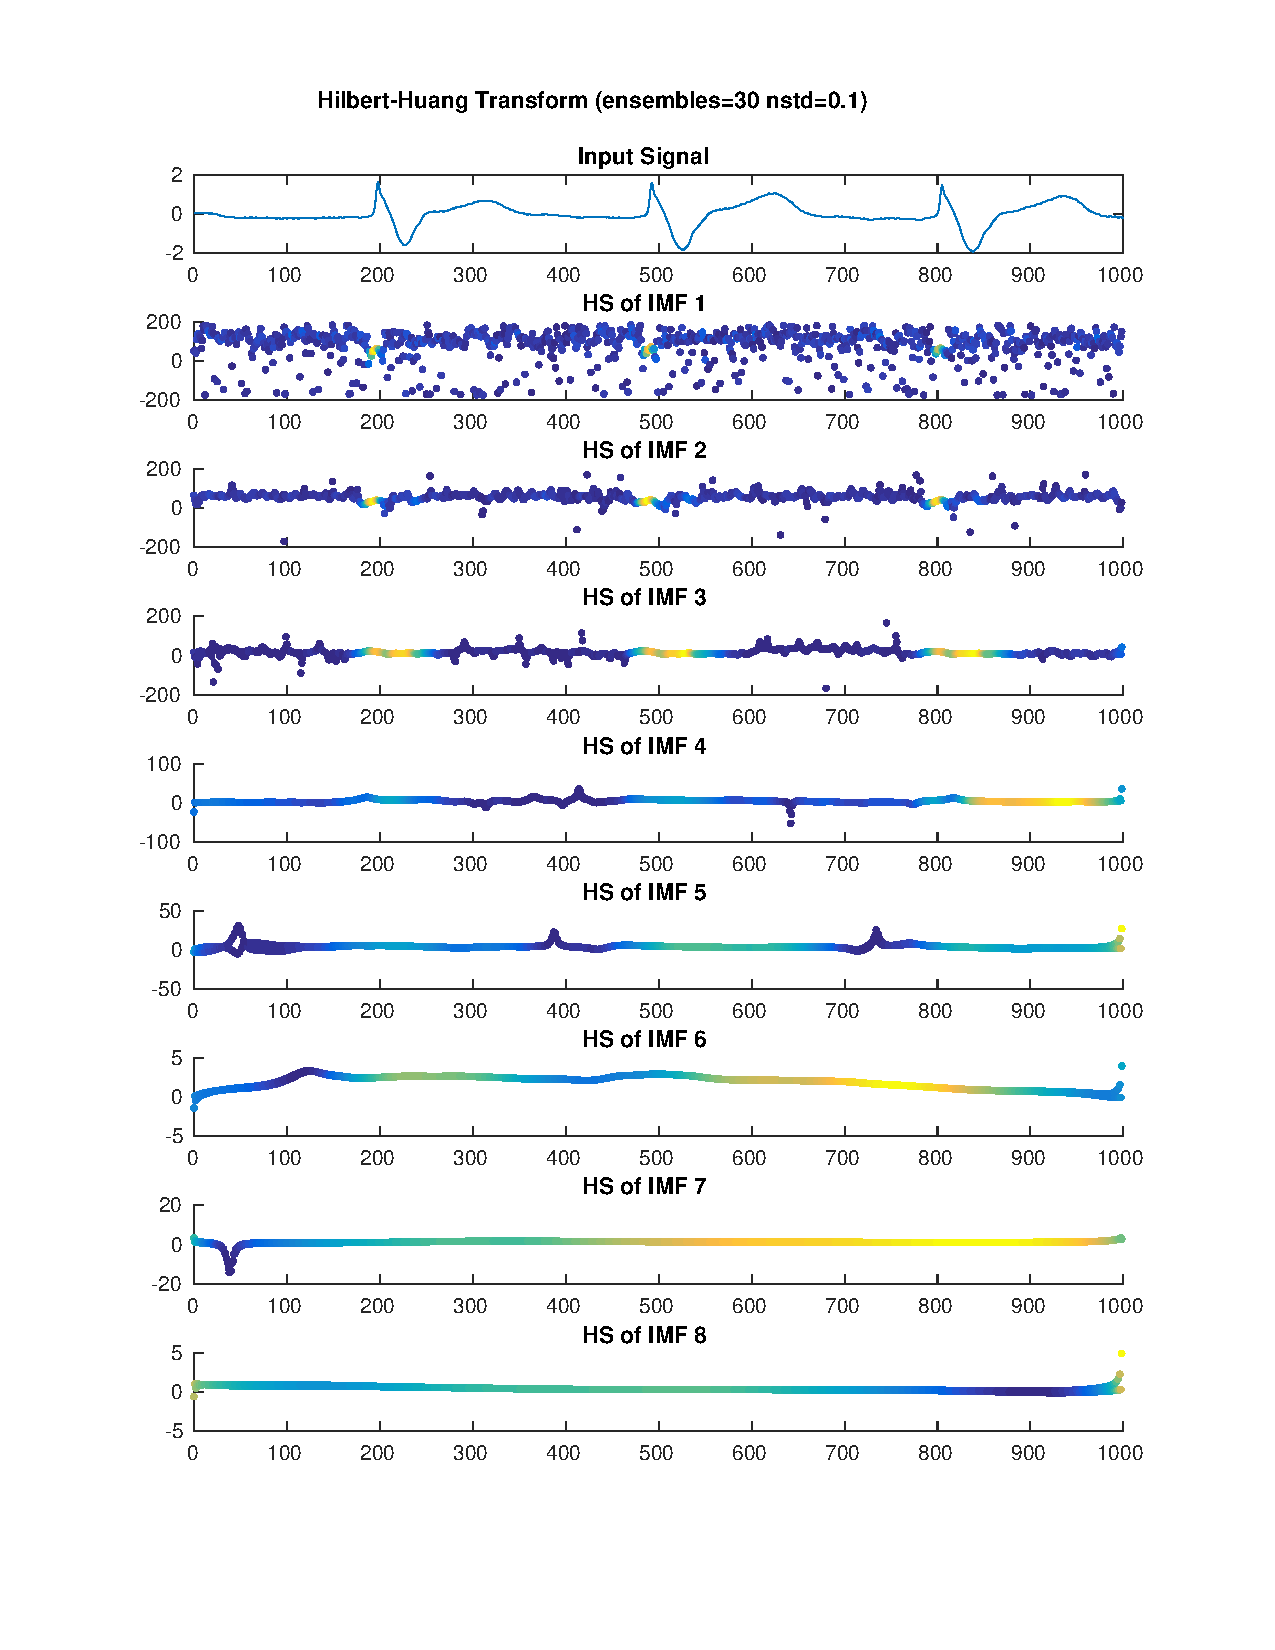
\includegraphics[width=\textwidth]{fig/217l1_hht_ensemble.pdf}
	
	(β)
\end{minipage}
\vfill
\caption{(α) Ensemble Emperical Mode Decomposition (β) Hilbert-Huang Transform του σήματος με $n_{ens}=50$ και $\sigma_n = 0.1$.}
\label{fig:217l1_hht_ensemble}
\end{figure}

\subsection*{221}

% --- STFT, WDF, CWT ---
\begin{figure}[H]
\centering
\begin{minipage}{0.48\textwidth}
	\centering
	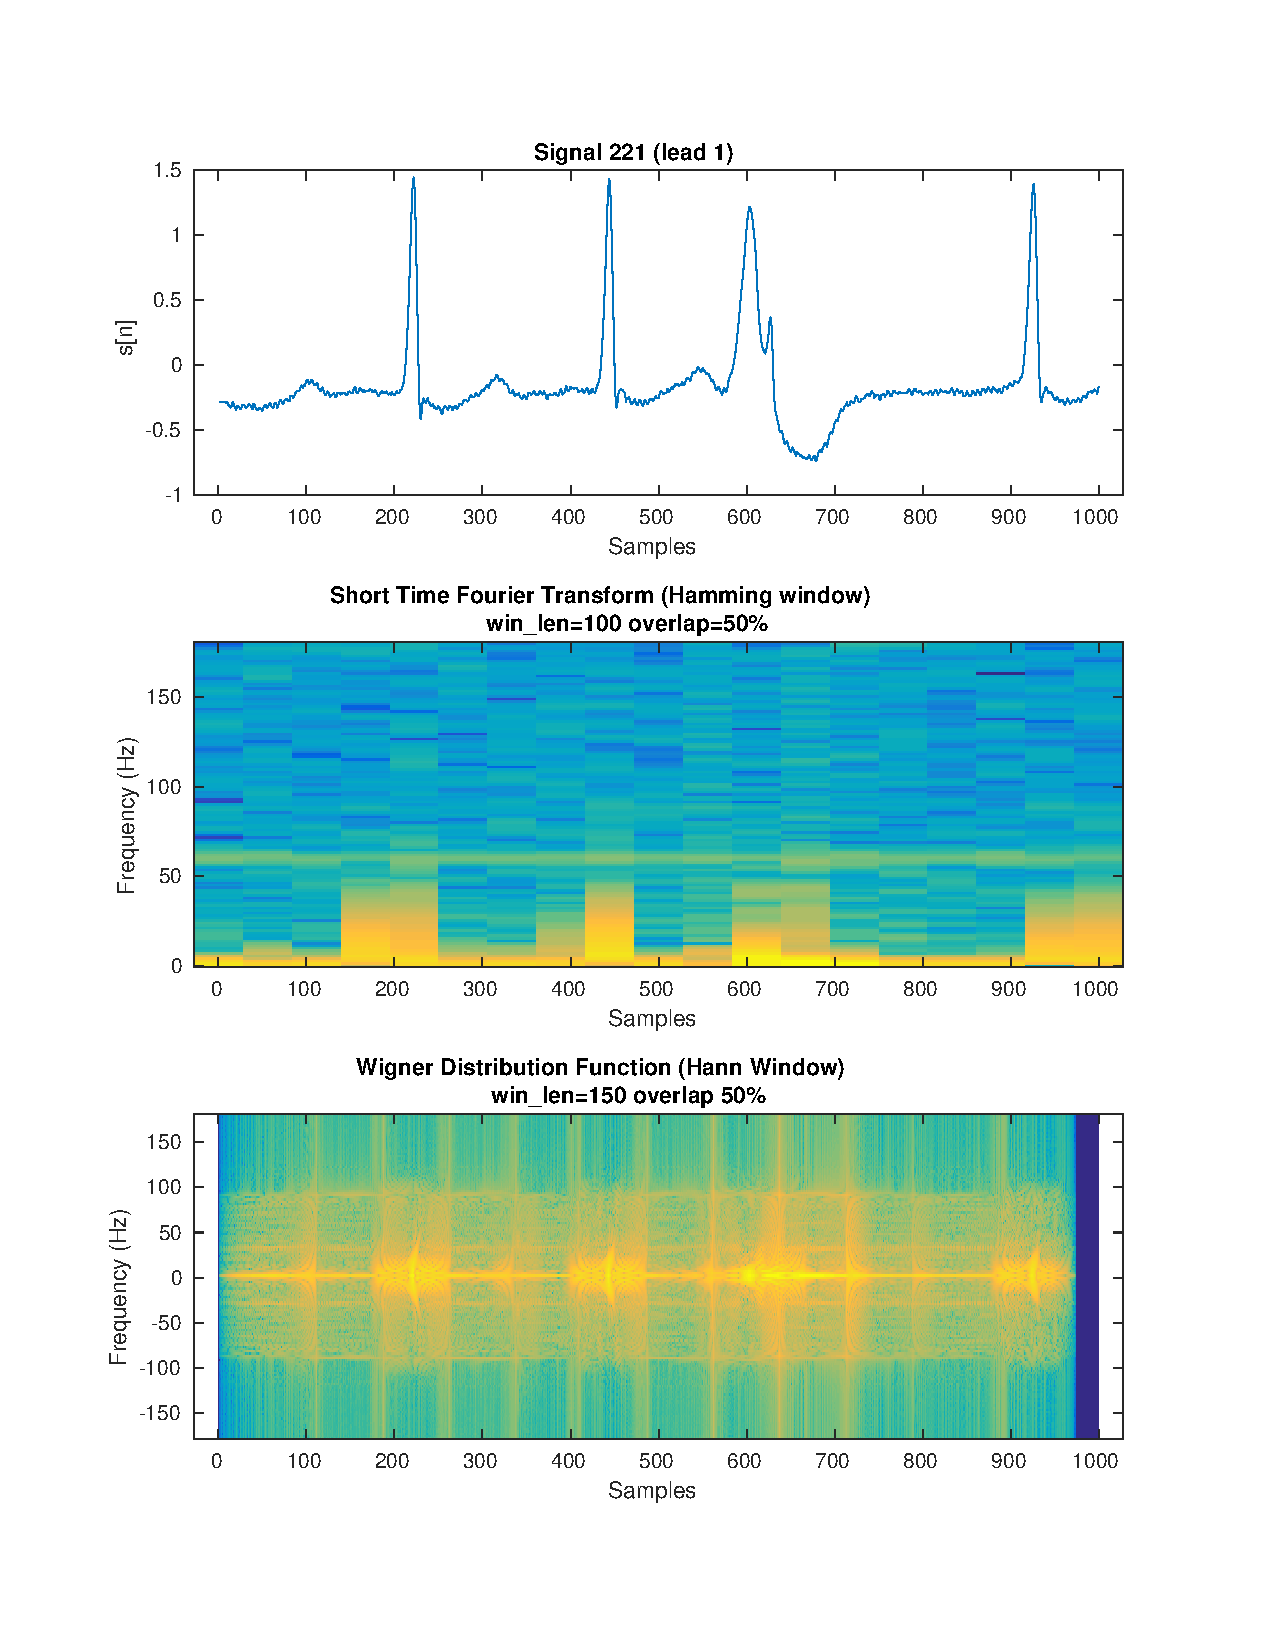
\includegraphics[width=\textwidth]{fig/221l1_stft_wdf.pdf}
	
	(α)
\end{minipage}
\begin{minipage}{0.48\textwidth}
	\centering
	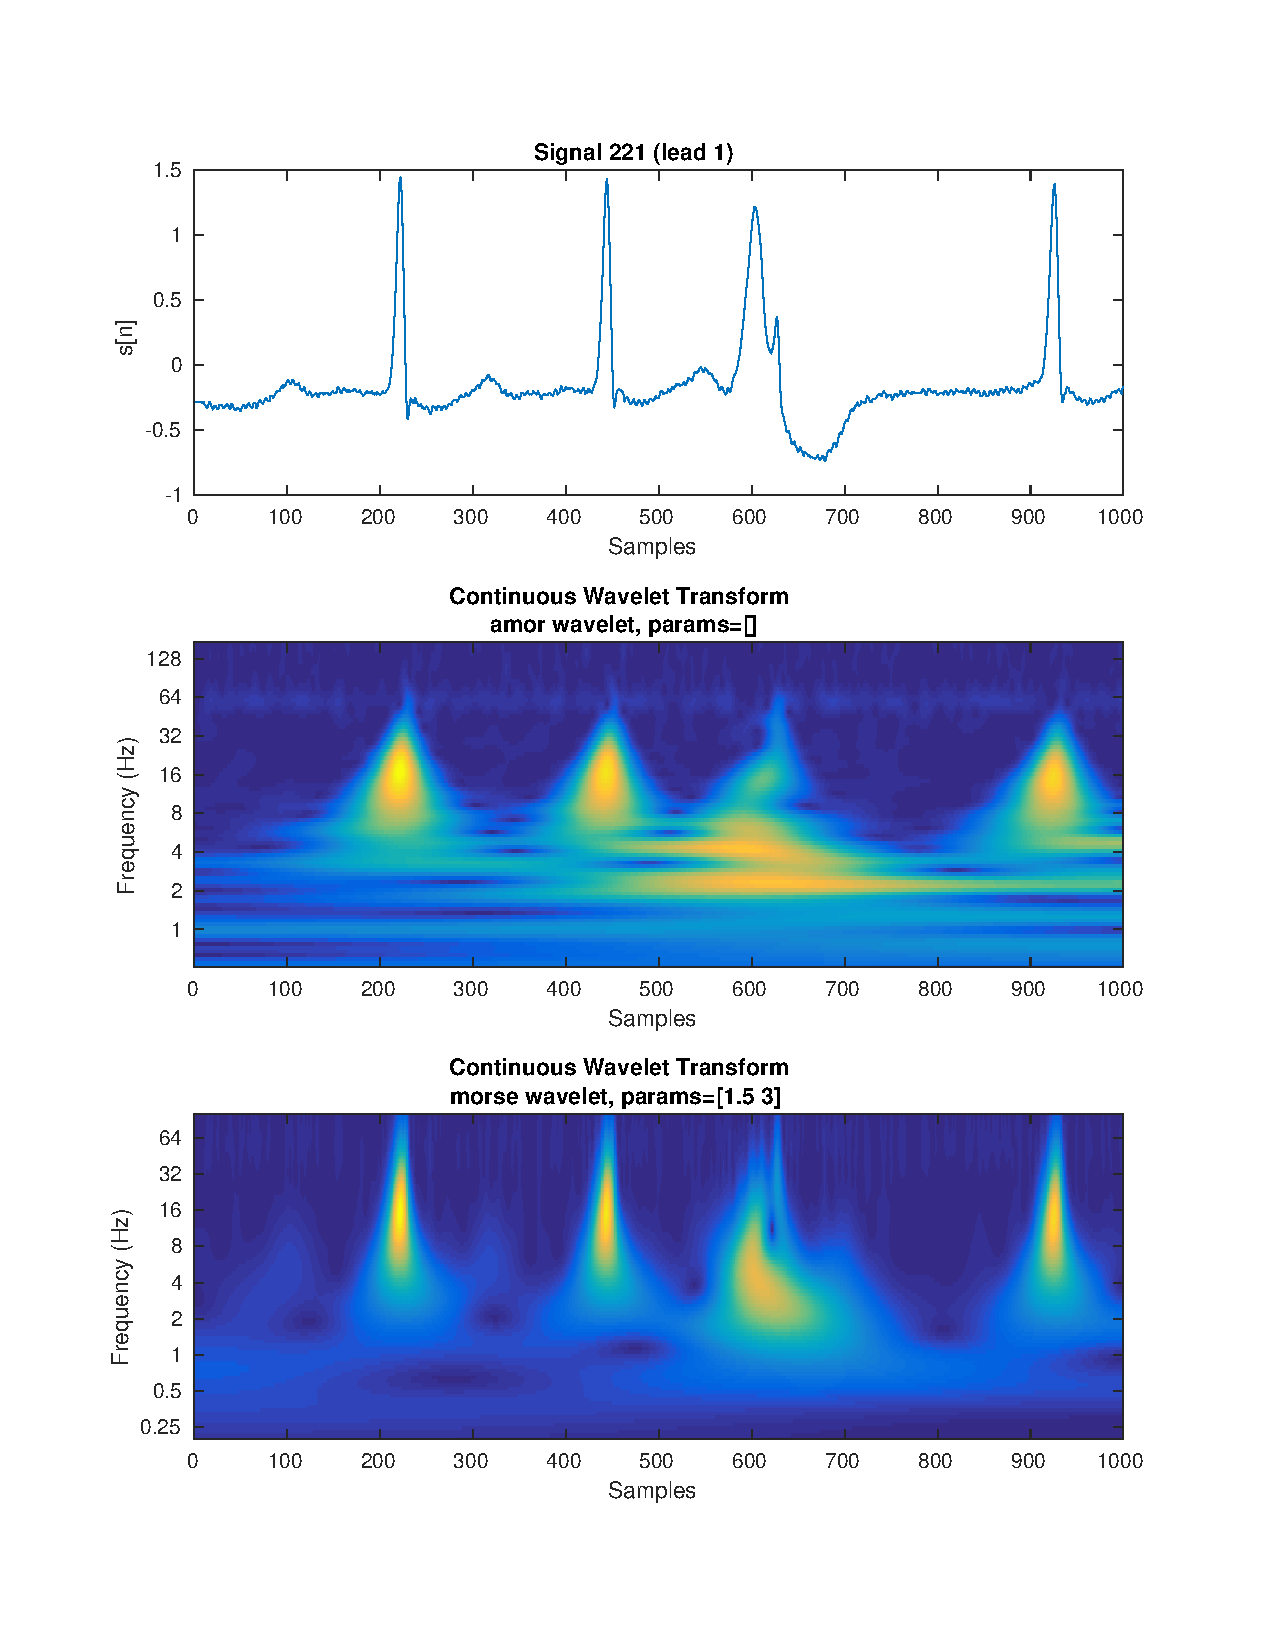
\includegraphics[width=\textwidth]{fig/221l1_cwt.pdf}
	
	(β)
\end{minipage}
\vfill
\caption{(α) Short Time Fourier Transform και Wigner Distribution Function (β) Wavelet Transform (Morlet, Morse wavelets) του σήματος.}
\label{fig:221l1_stft_wdf_wt}
\end{figure}


% --- DWT ---
\begin{figure}[H]
\centering
\begin{minipage}{0.48\textwidth}
	\centering
	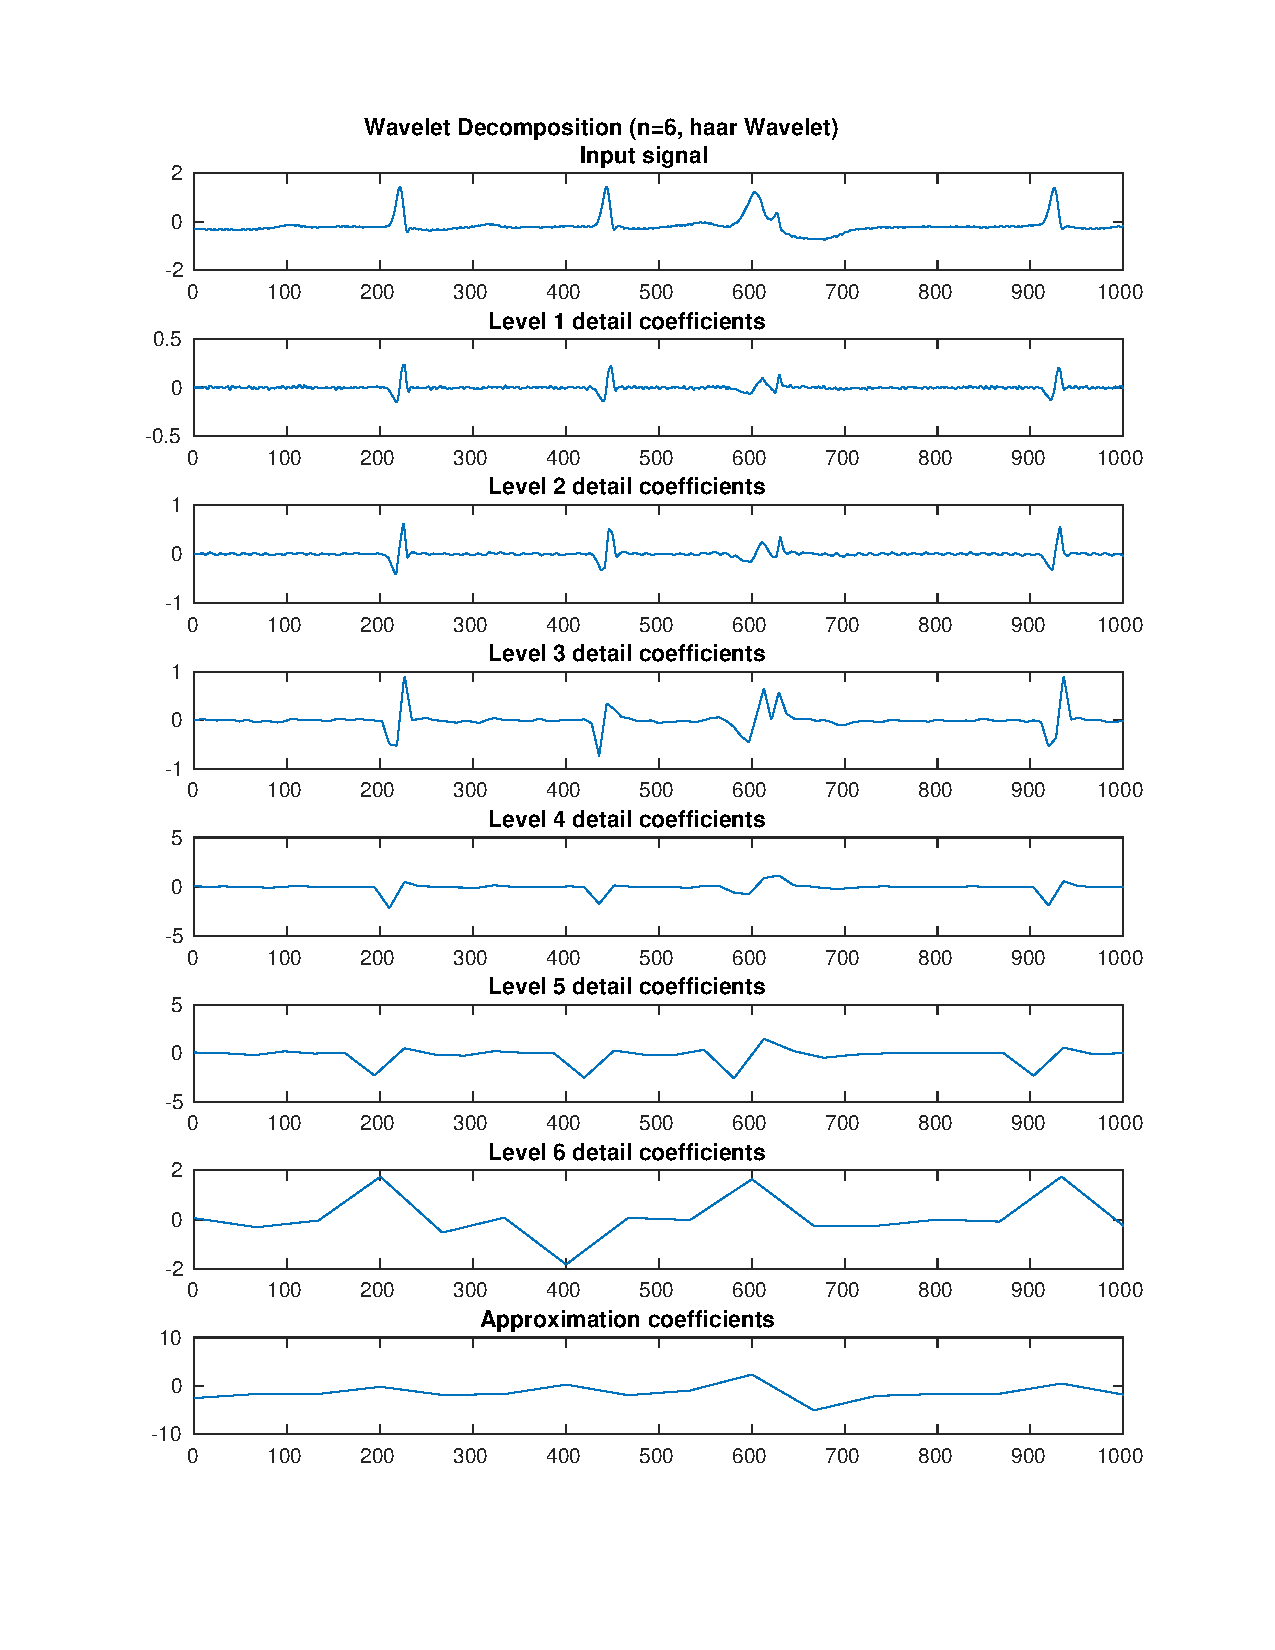
\includegraphics[width=\textwidth]{fig/221l1_dwt1.pdf}
	
	(α)
\end{minipage}
\begin{minipage}{0.48\textwidth}
	\centering
	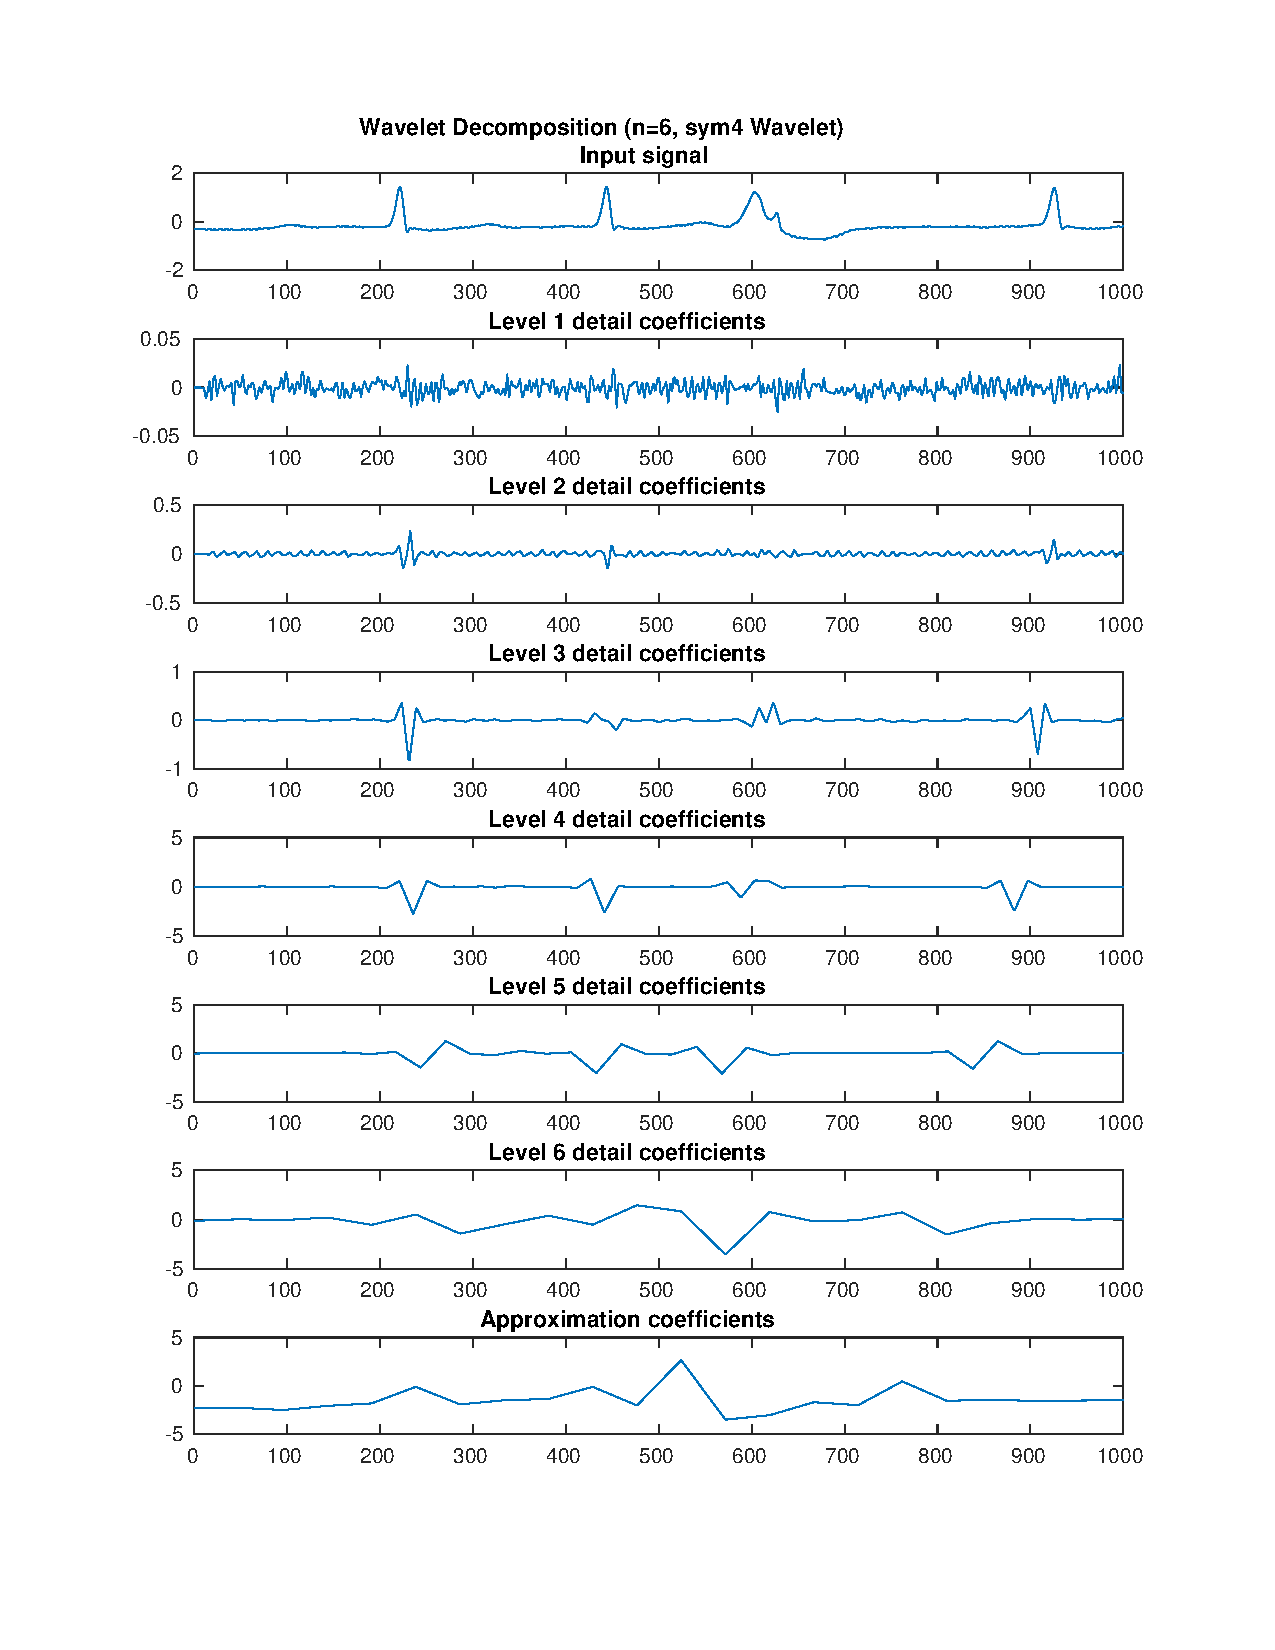
\includegraphics[width=\textwidth]{fig/221l1_dwt2.pdf}
	
	(β)
\end{minipage}
\vfill
\caption{Wavelet Decomposition του σήματος χρησιμοποιώντας wavelet (α) Haar (β) Symlet4.}
\label{fig:221l1_dwt}
\end{figure}


% --- EMD/HHT ---
\begin{figure}[H]
\centering
\begin{minipage}{0.48\textwidth}
	\centering
	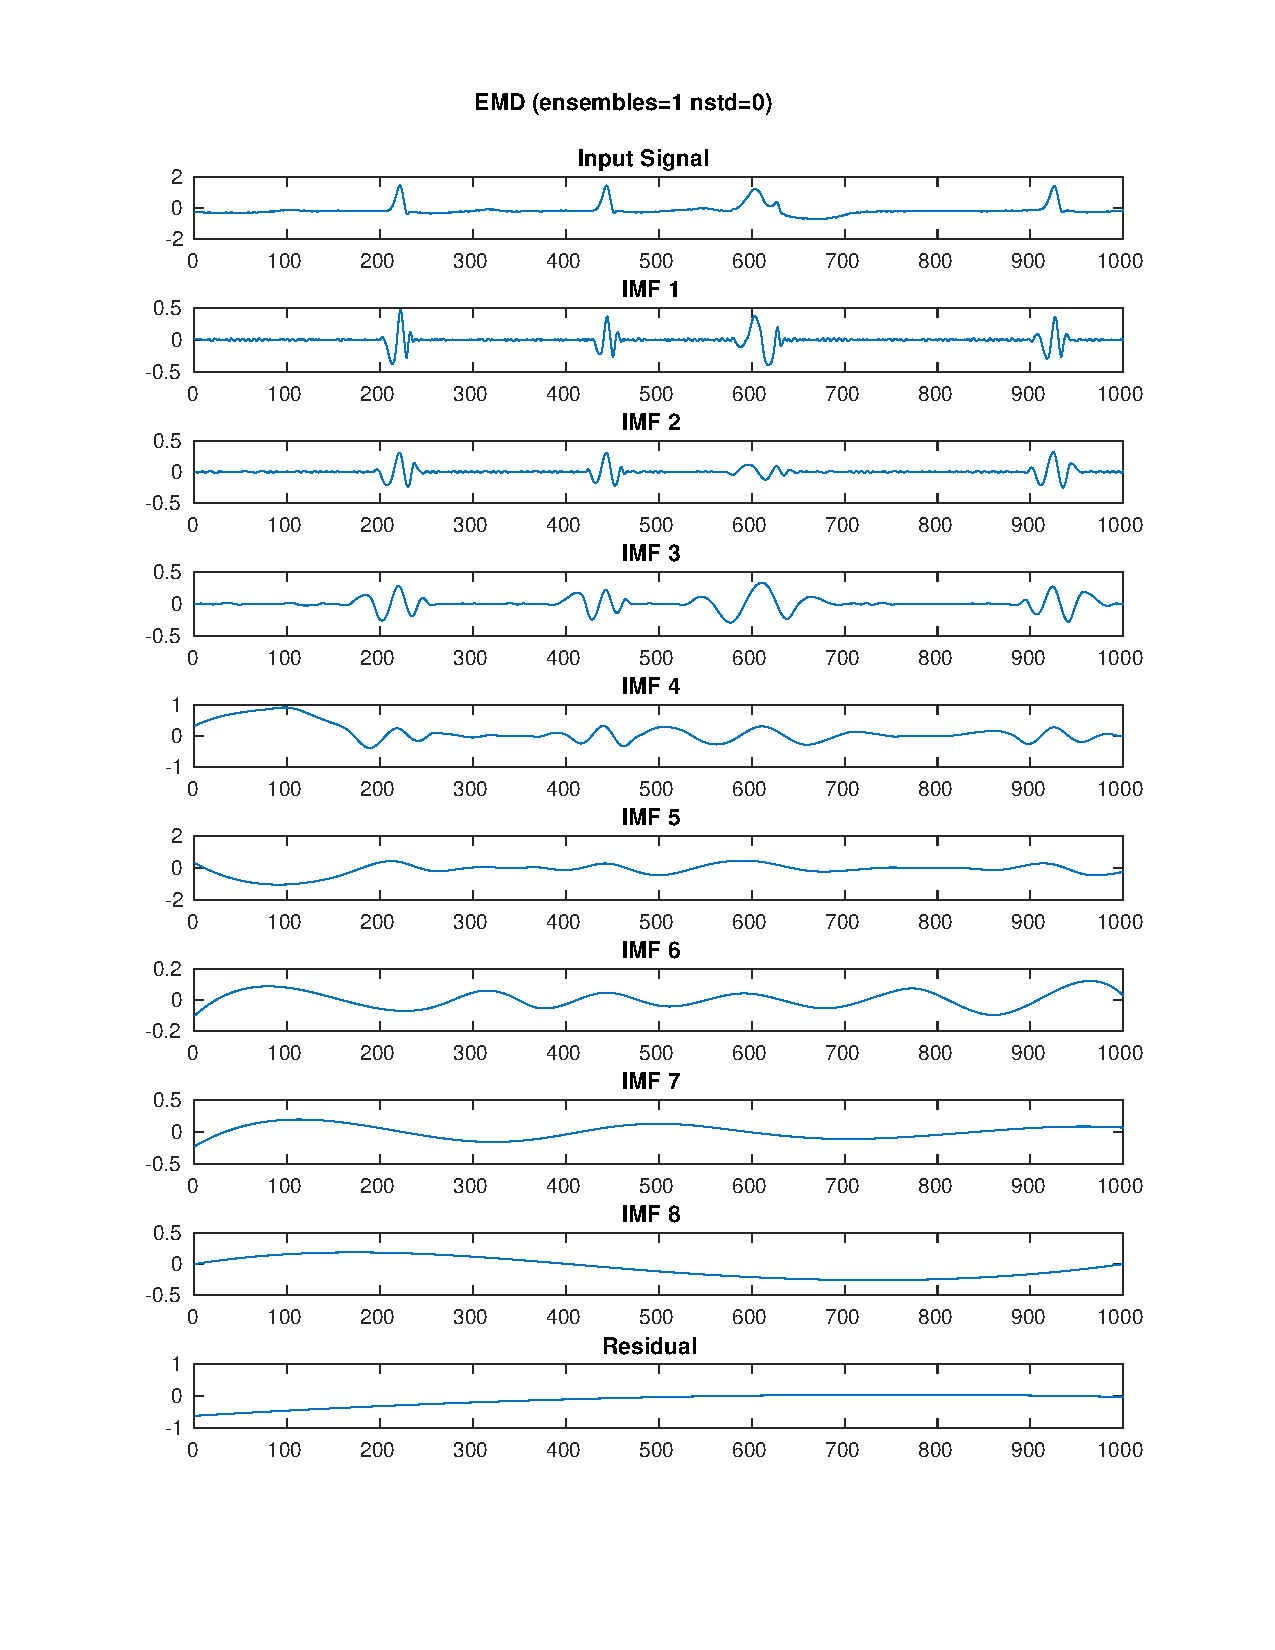
\includegraphics[width=\textwidth]{fig/221l1_emd.pdf}
	
	(α)
\end{minipage}
\begin{minipage}{0.48\textwidth}
	\centering
	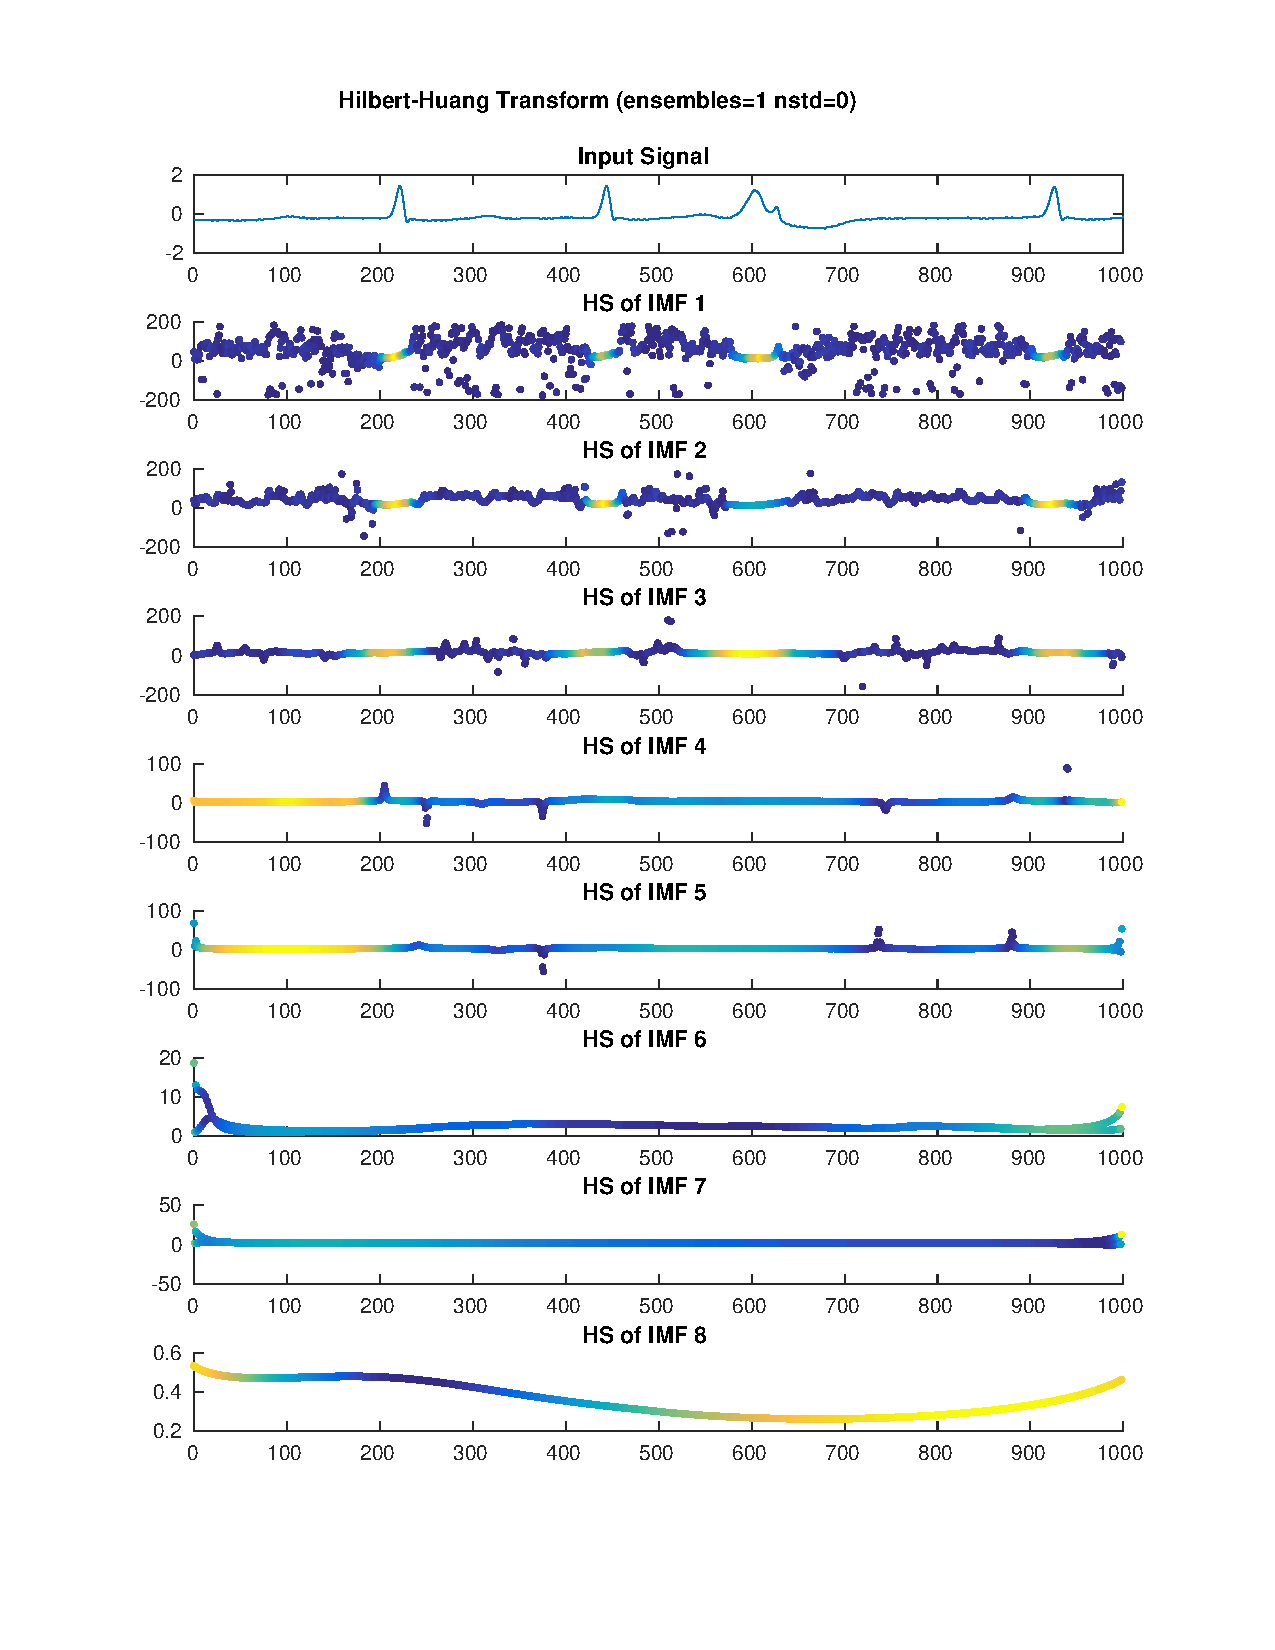
\includegraphics[width=\textwidth]{fig/221l1_hht.pdf}
	
	(β)
\end{minipage}
\vfill
\caption{(α) Emperical Mode Decomposition (β) Hilbert-Huang Transform του σήματος.}
\label{fig:221l1_hht}
\end{figure}


% --- EEMD/HHT ---
\begin{figure}[H]
\centering
\begin{minipage}{0.48\textwidth}
	\centering
	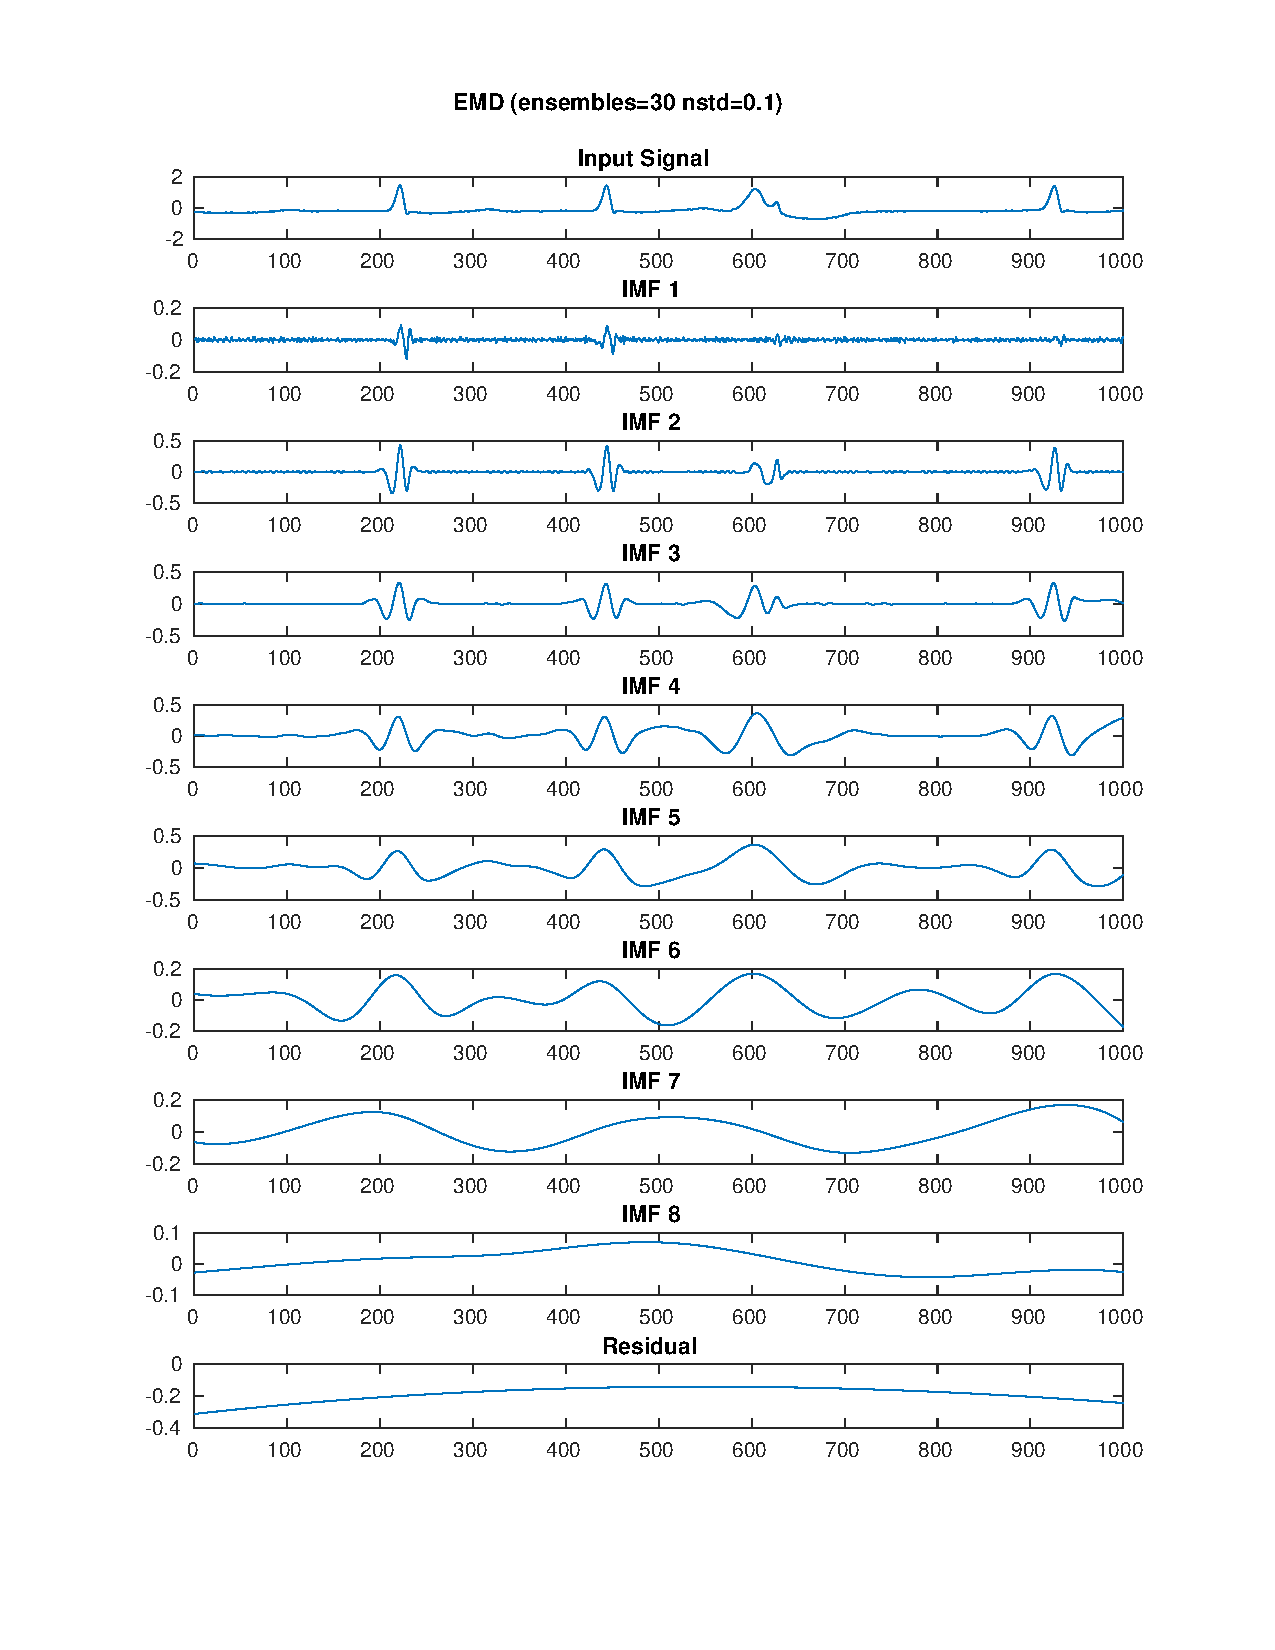
\includegraphics[width=\textwidth]{fig/221l1_emd_ensemble.pdf}
	
	(α)
\end{minipage}
\begin{minipage}{0.48\textwidth}
	\centering
	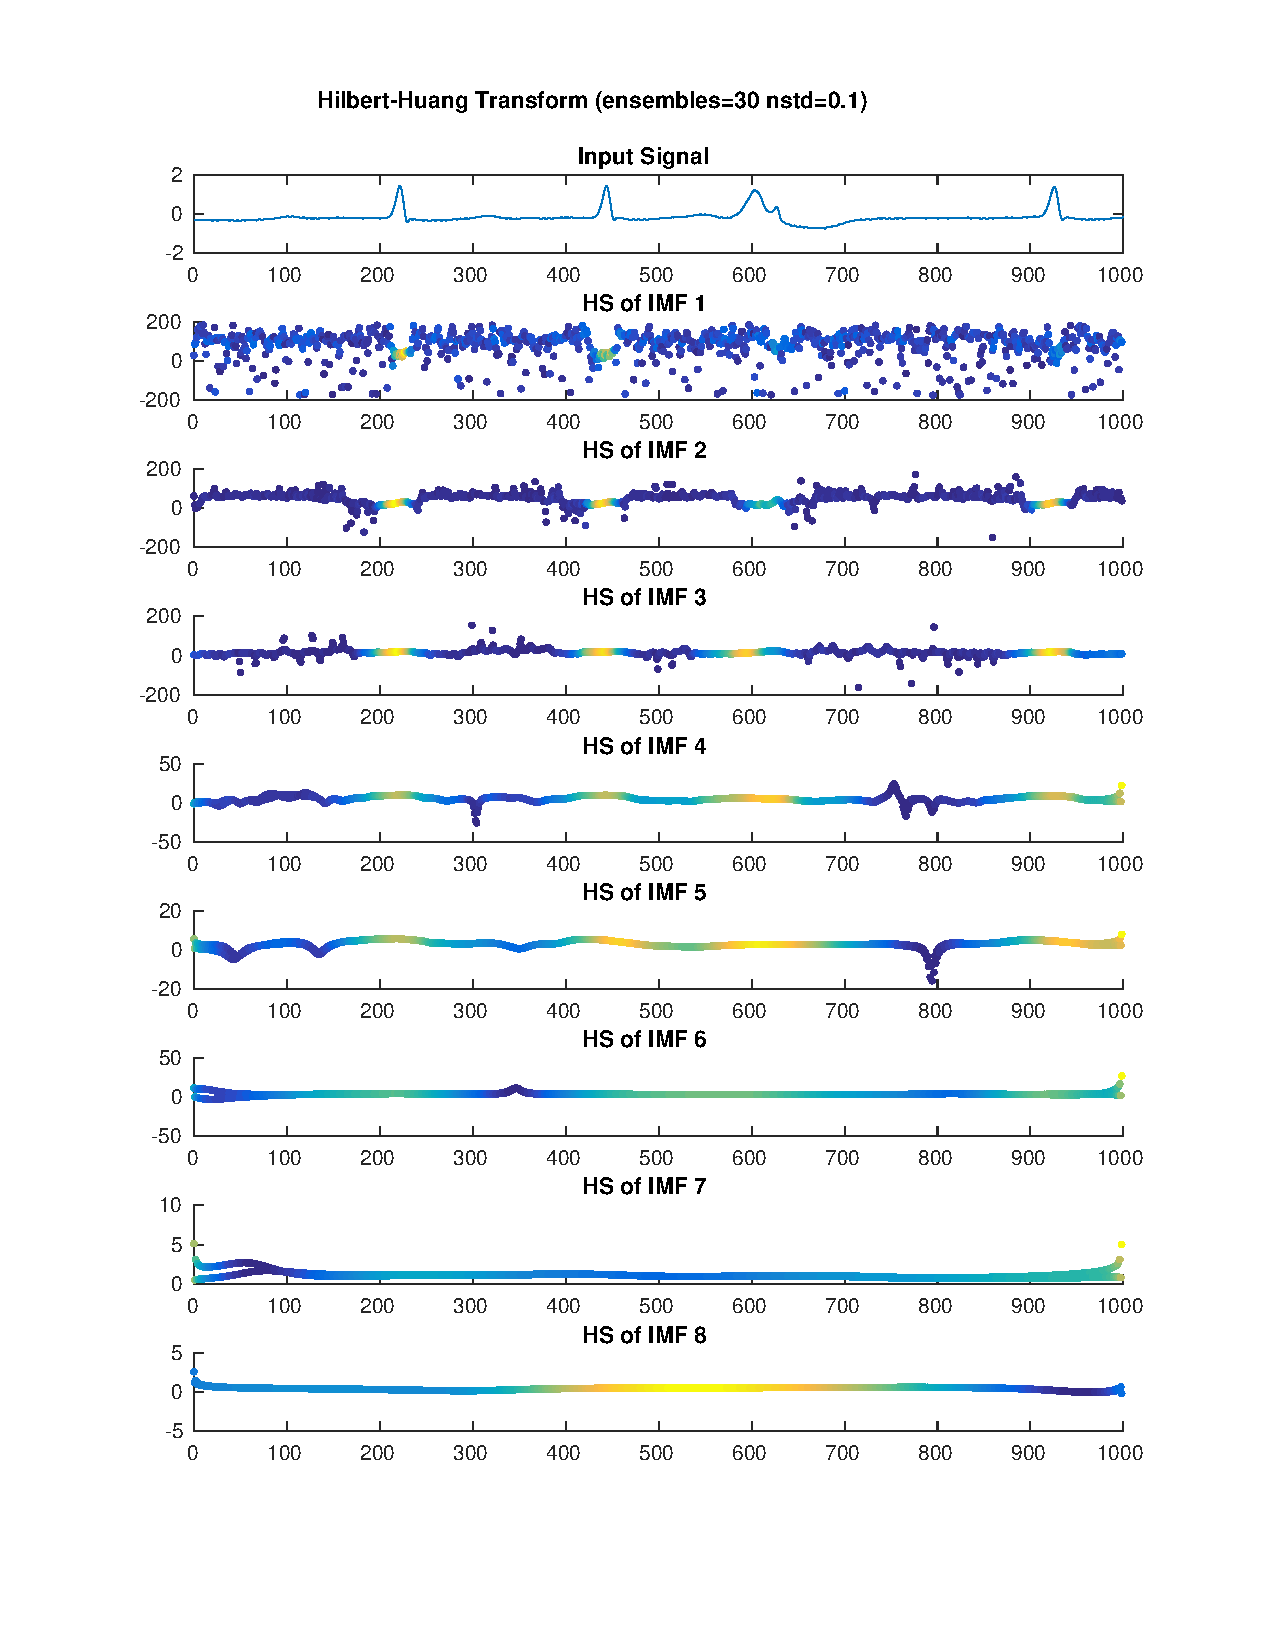
\includegraphics[width=\textwidth]{fig/221l1_hht_ensemble.pdf}
	
	(β)
\end{minipage}
\vfill
\caption{(α) Ensemble Emperical Mode Decomposition (β) Hilbert-Huang Transform του σήματος με $n_{ens}=50$ και $\sigma_n = 0.1$.}
\label{fig:221l1_hht_ensemble}
\end{figure}

\end{document}